%%%%%%%%%%%%%%%%%%%%%%%%%%%%%%%%%%%%%%%%%%%%%%%%%%%%%%%%%%%%
%%  Presentation for the seminar `Language and Brain`
%%  
%%    
%%
%%  Friedrich Schuessler
%%  January 2016

\documentclass[xcolor=x11names,compress]{beamer}
\usepackage[utf8]{inputenc} 
\usepackage[T1]{fontenc}
\usepackage{cmbright}

%% General document %%%%%%%%%%%%%%%%%%%%%%%%%%%%%%%%%%
\usepackage{graphicx}
\usepackage{caption}  
\usepackage{subcaption}     % subfloats
\usepackage{amsmath,mathtools}  % math stuff

\usepackage{tikz}

\usepackage[style=authoryear]{biblatex}
\usetikzlibrary{decorations.fractals}

%%% Set path for figures
%\graphicspath{{../full_pdf/}}
\graphicspath{{../figures/}}
\DeclareGraphicsExtensions{.pdf,.png,.jpg, .eps}
%%%%%%%%%%%%%%%%%%%%%%%%%%%%%%%%%%%%%%%%%%%%%%%%%%%%%%


%% Beamer Layout %%%%%%%%%%%%%%%%%%%%%%%%%%%%%%%%%%
\useoutertheme[subsection=false,shadow]{miniframes}
\setbeamerfont{title like}{shape=\scshape}
\setbeamerfont{frametitle}{shape=\scshape}

\setbeamercolor*{lower separation line head}{bg=DeepSkyBlue4} 
\setbeamercolor*{normal text}{fg=black,bg=white} 
\setbeamercolor*{alerted text}{fg=red} 
\setbeamercolor*{example text}{fg=black} 
\setbeamercolor*{structure}{fg=black} 

\usenavigationsymbolstemplate{}
\setbeamercolor*{palette tertiary}{fg=black,bg=black!10} 
\setbeamercolor*{palette quaternary}{fg=black,bg=black!10} 

\setbeamercovered{dynamic} % enable pause

\renewcommand{\(}{\begin{columns}}
\renewcommand{\)}{\end{columns}}
\newcommand{\<}[1]{\begin{column}{#1}}
\renewcommand{\>}{\end{column}}
%%%%%%%%%%%%%%%%%%%%%%%%%%%%%%%%%%%%%%%%%%%%%%%%%%
\useoutertheme{infolines} % authors, etc.

% Hide the "/ N" in slide "n / N":
\makeatletter 
\setbeamertemplate{footline}
{
  \leavevmode%
  \hbox{%
  %\begin{beamercolorbox}[wd=.333333\paperwidth,ht=2.25ex,dp=1ex,center]{author in head/foot}%
    %\usebeamerfont{author in head/foot}\insertshortauthor~~\beamer@ifempty{\insertshortinstitute}{}{(\insertshortinstitute)}
  %\end{beamercolorbox}%
  \begin{beamercolorbox}[wd=.666666\paperwidth,ht=2.25ex,dp=1ex,center]{title in head/foot}%
    \usebeamerfont{title in head/foot}\insertshorttitle
  \end{beamercolorbox}%
  \begin{beamercolorbox}[wd=.333333\paperwidth,ht=2.25ex,dp=1ex,right]{}%
    \usebeamerfont{date in head/foot}\hspace*{2em}
    \insertframenumber\hspace*{2ex} 
  \end{beamercolorbox}}%
  \vskip0pt%
}
\makeatother
%%%%%%%%%%%%%%%%%%%%%%%%%%%%%%%%%%%%%%%%%%%%%%%%%%

\bibliography{presentation.bib}

\DeclareGraphicsExtensions{.pdf,.png,.jpg, .eps}

%%%%%%%%%%%%%%%%%%%%%%%%%%%%%%%%%%%%%%%%%%%%%%%%%%%%%
% My own definitions
\usepackage{color, colortbl}  
\definecolor{TableColor}{HTML}{A1D99B}

% Math stuff
\newcommand*\diff{\mathop{}\!\text{d}}
\newcommand*\Diff[1]{\mathop{}\!\text{d^#1}}
\DeclareMathOperator{\Tr}{Tr} % Trace

%%%%%%%%%%%%%%%%%%%%%%%%%%%%%%%%%%%%%%%%%%%%%%%%%%%%%%%
\begin{document}

\begin{frame}{}
\title[FM]{The  visual  system  of  rodents: \\
How are neuronal    networks    in  the visual cortex  changed by  visual  experience?}
\subtitle{Part II}
\author{
Jun Okada \& Friedrich Schüßler}
\date{\normalsize 28 January 2016}
%\date{\today}
\titlepage

\centering 
Coach: Stefan Rotter
\end{frame}

\begin{frame}{Table of contents}
    \tableofcontents
\end{frame}

%% Show Table of Contents at the beginning of each section
%\AtBeginSection[]{
%\begin{frame}{Table of contents}
    %\tableofcontents[currentsection]
%\end{frame}
%}

%%%%%%%%%%%%%%%%%%% Start
%%%%%%%%%%%%%%%%%%%%%%%%%%%%%%%%%%%%%%%%%%%%%%%%%%%%%%%%%%%%%%%%%%%%
\section{Why the visual cortex?}
\label{sec:why_the_visual_cortex_}

% Language in the brain
\begin{frame}[t]{Language in the brain}
\begin{center}
    \only<1>{
    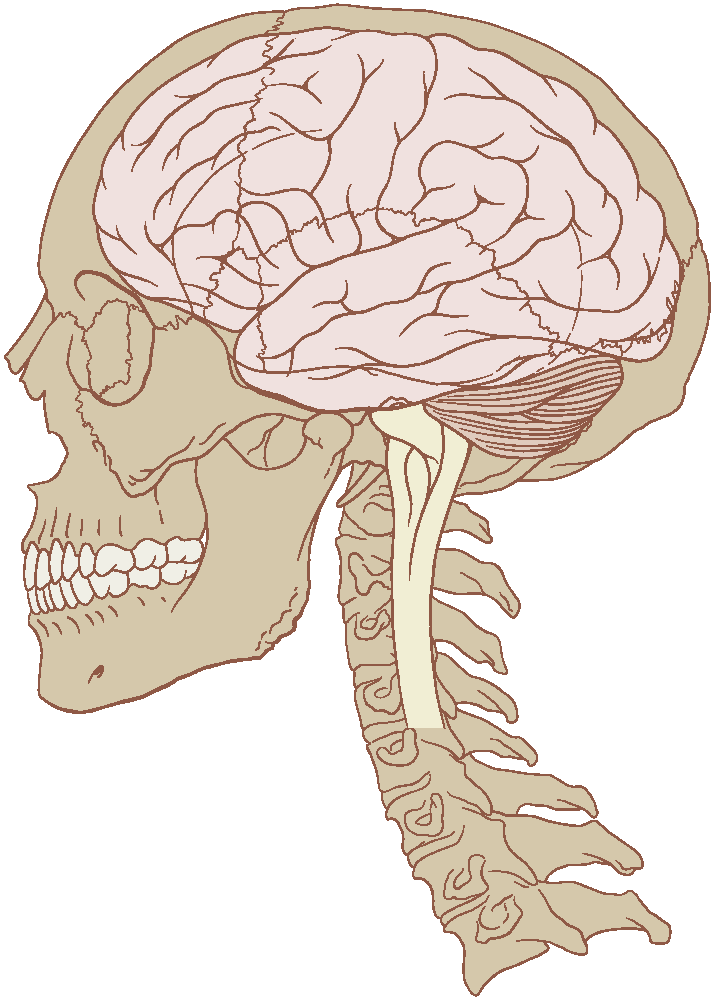
\includegraphics[height=0.9\textheight]{brain1}
    }
    %\only<2>{
    %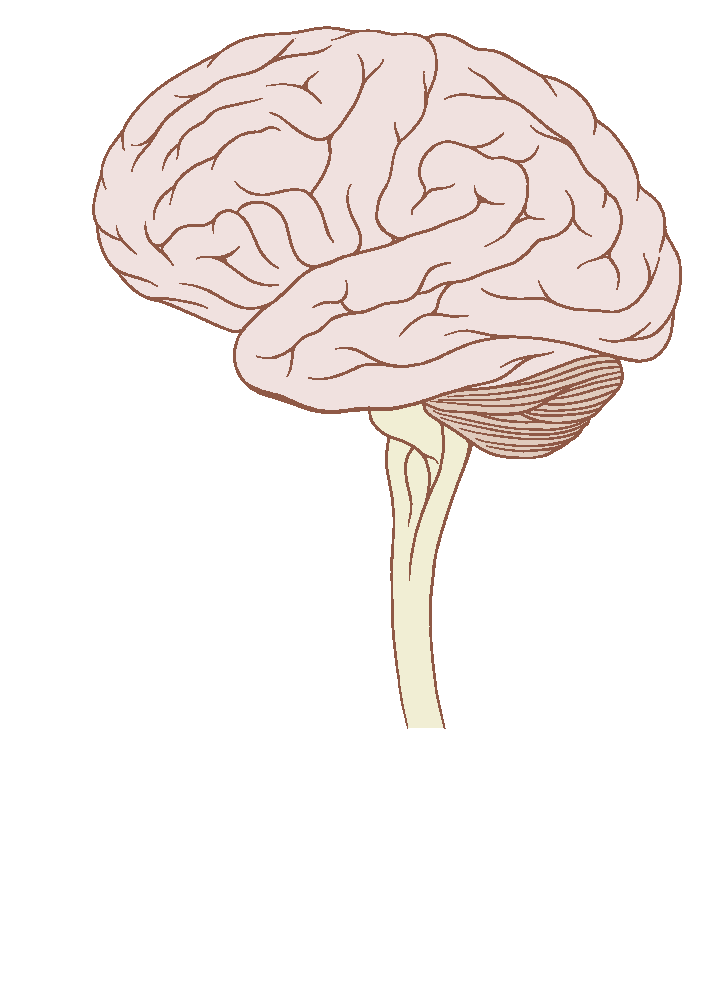
\includegraphics[height=0.9\textheight]{brain2}
    %}
    \only<2>{
    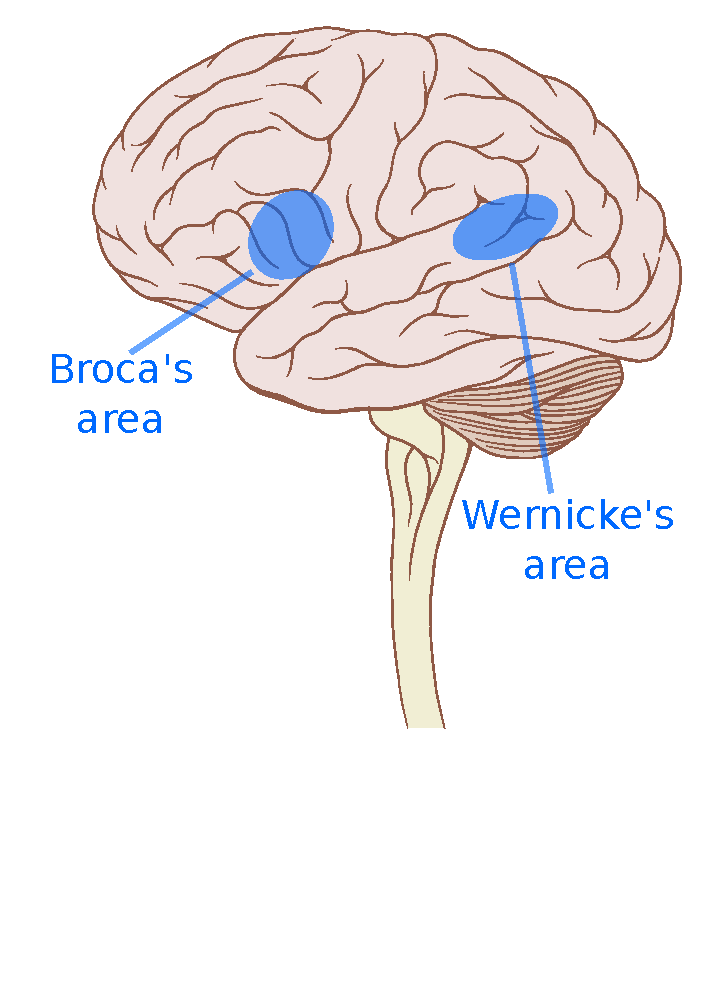
\includegraphics[height=0.9\textheight]{brain3}
    }
    \only<3>{
    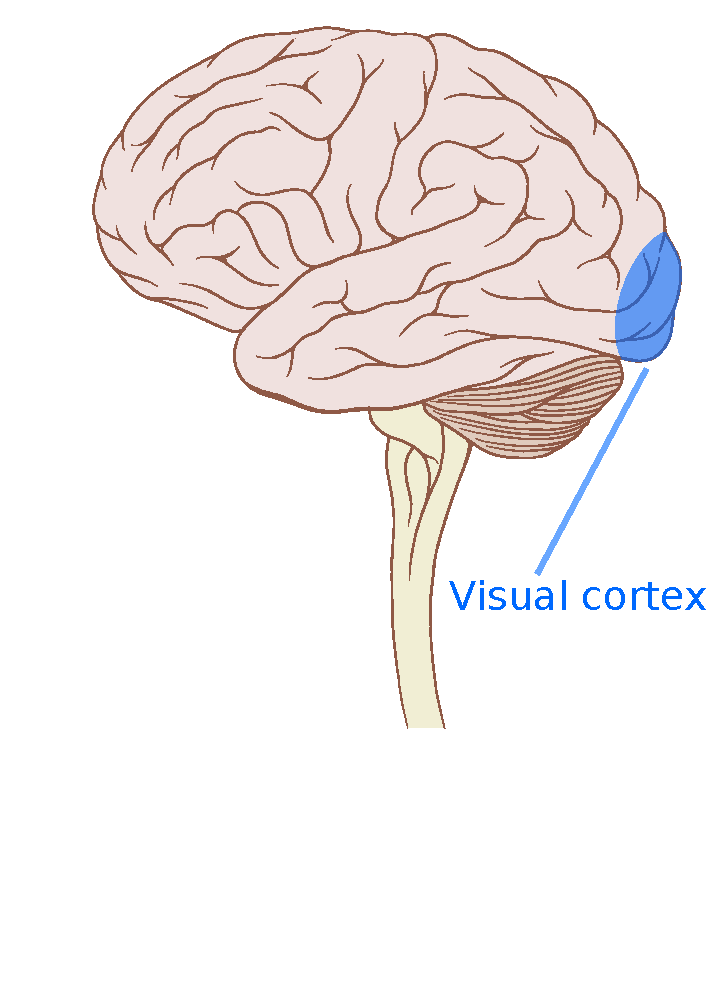
\includegraphics[height=0.9\textheight]{brain4}
    }
    \only<4>{
    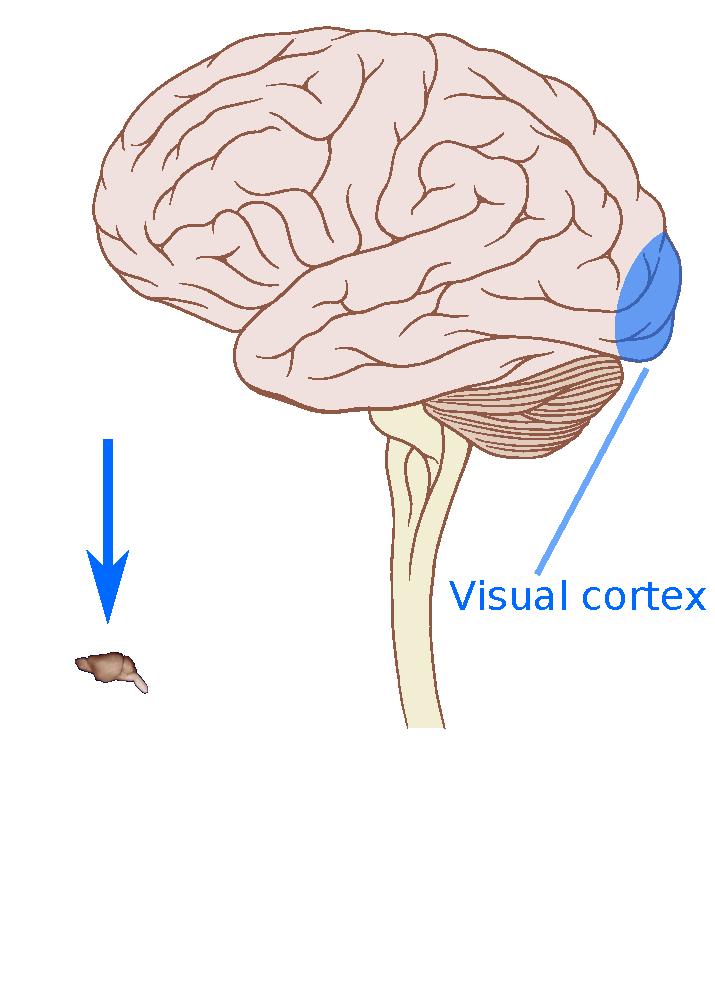
\includegraphics[height=0.9\textheight]{brain5}
    }
\end{center}
\end{frame}

% Mouse Visual Cortex
\begin{frame}[t]{Visual cortex in the mouse}
    \only<1>{
    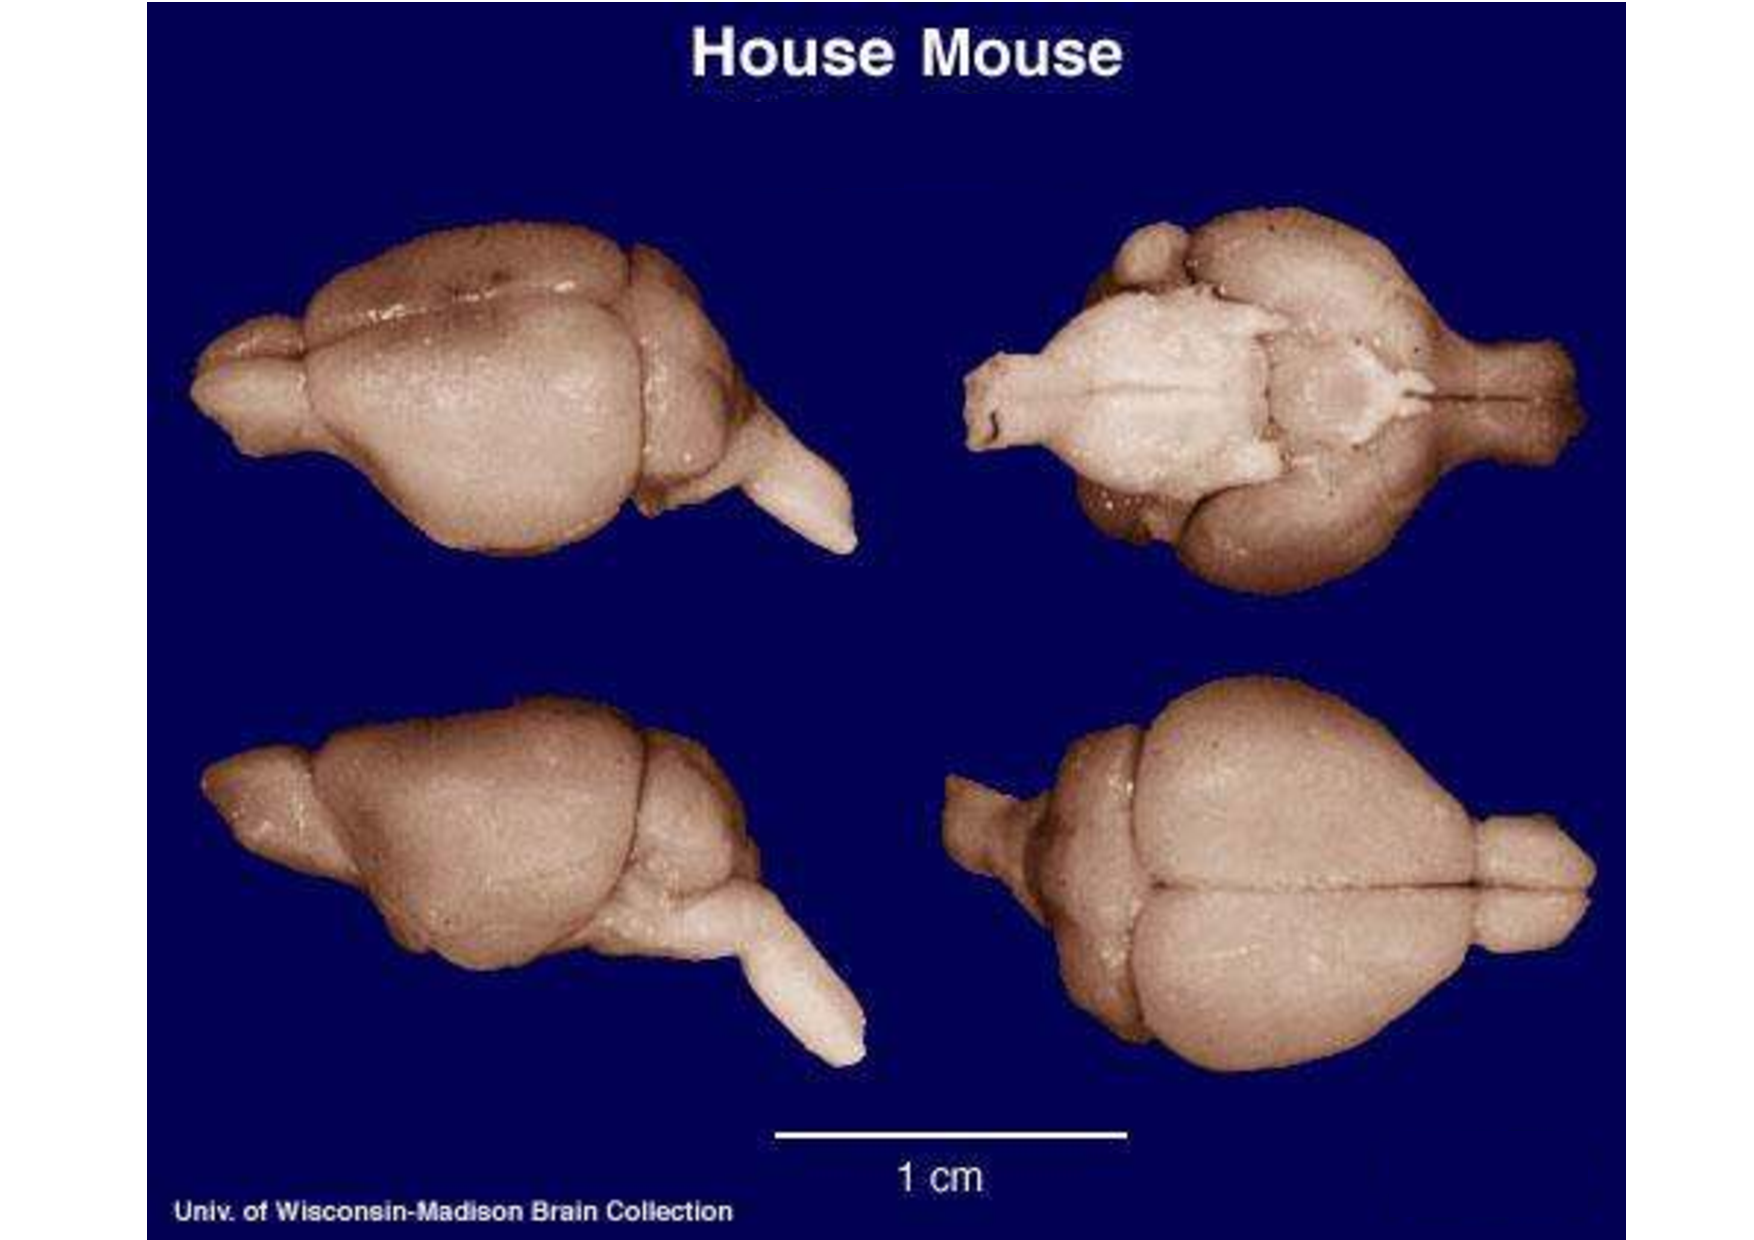
\includegraphics[height=0.9\textheight]{mouse1}
    }
    \only<2>{
    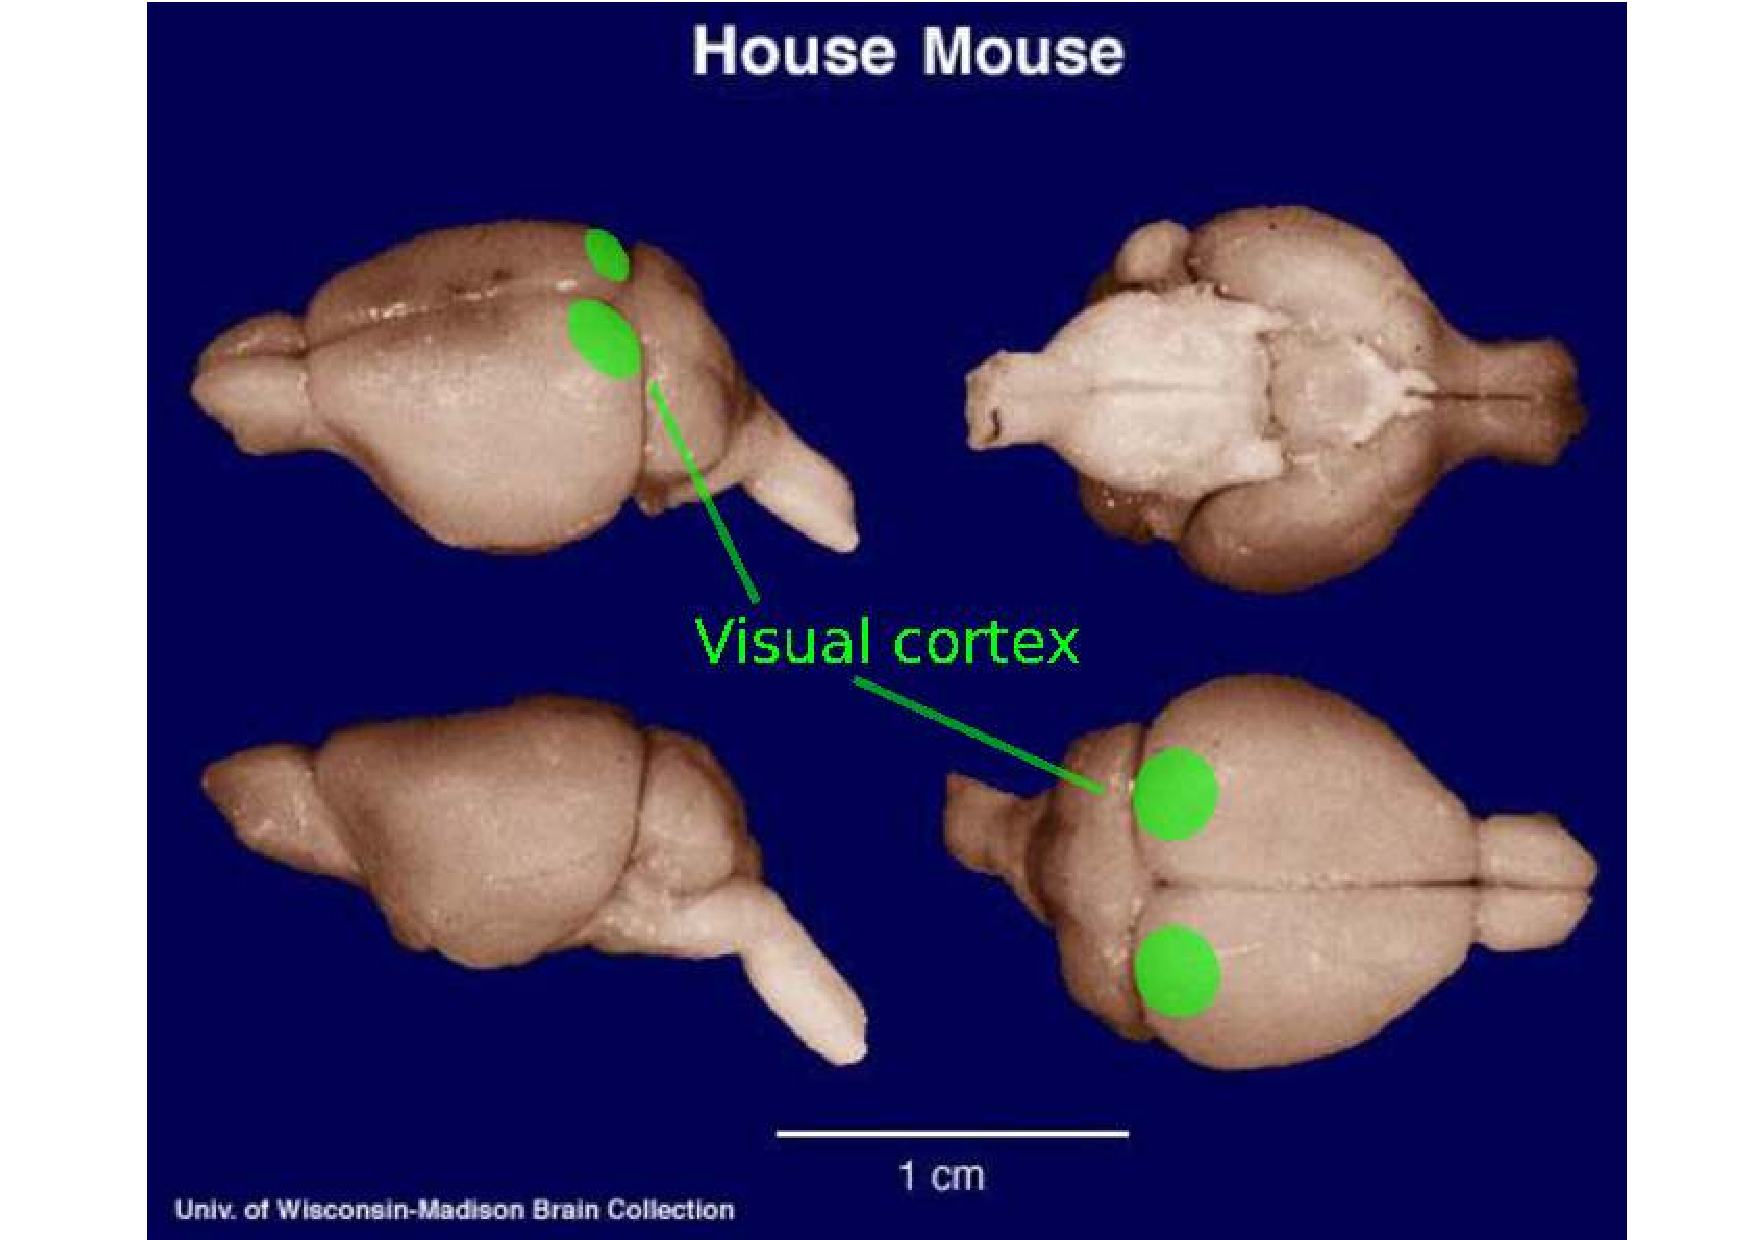
\includegraphics[height=0.9\textheight]{mouse2}
    }
\end{frame}

% Structure of visual cortex: Layer
\begin{frame}[t]{Universal structure of the neocortex}
    \only<1>{
    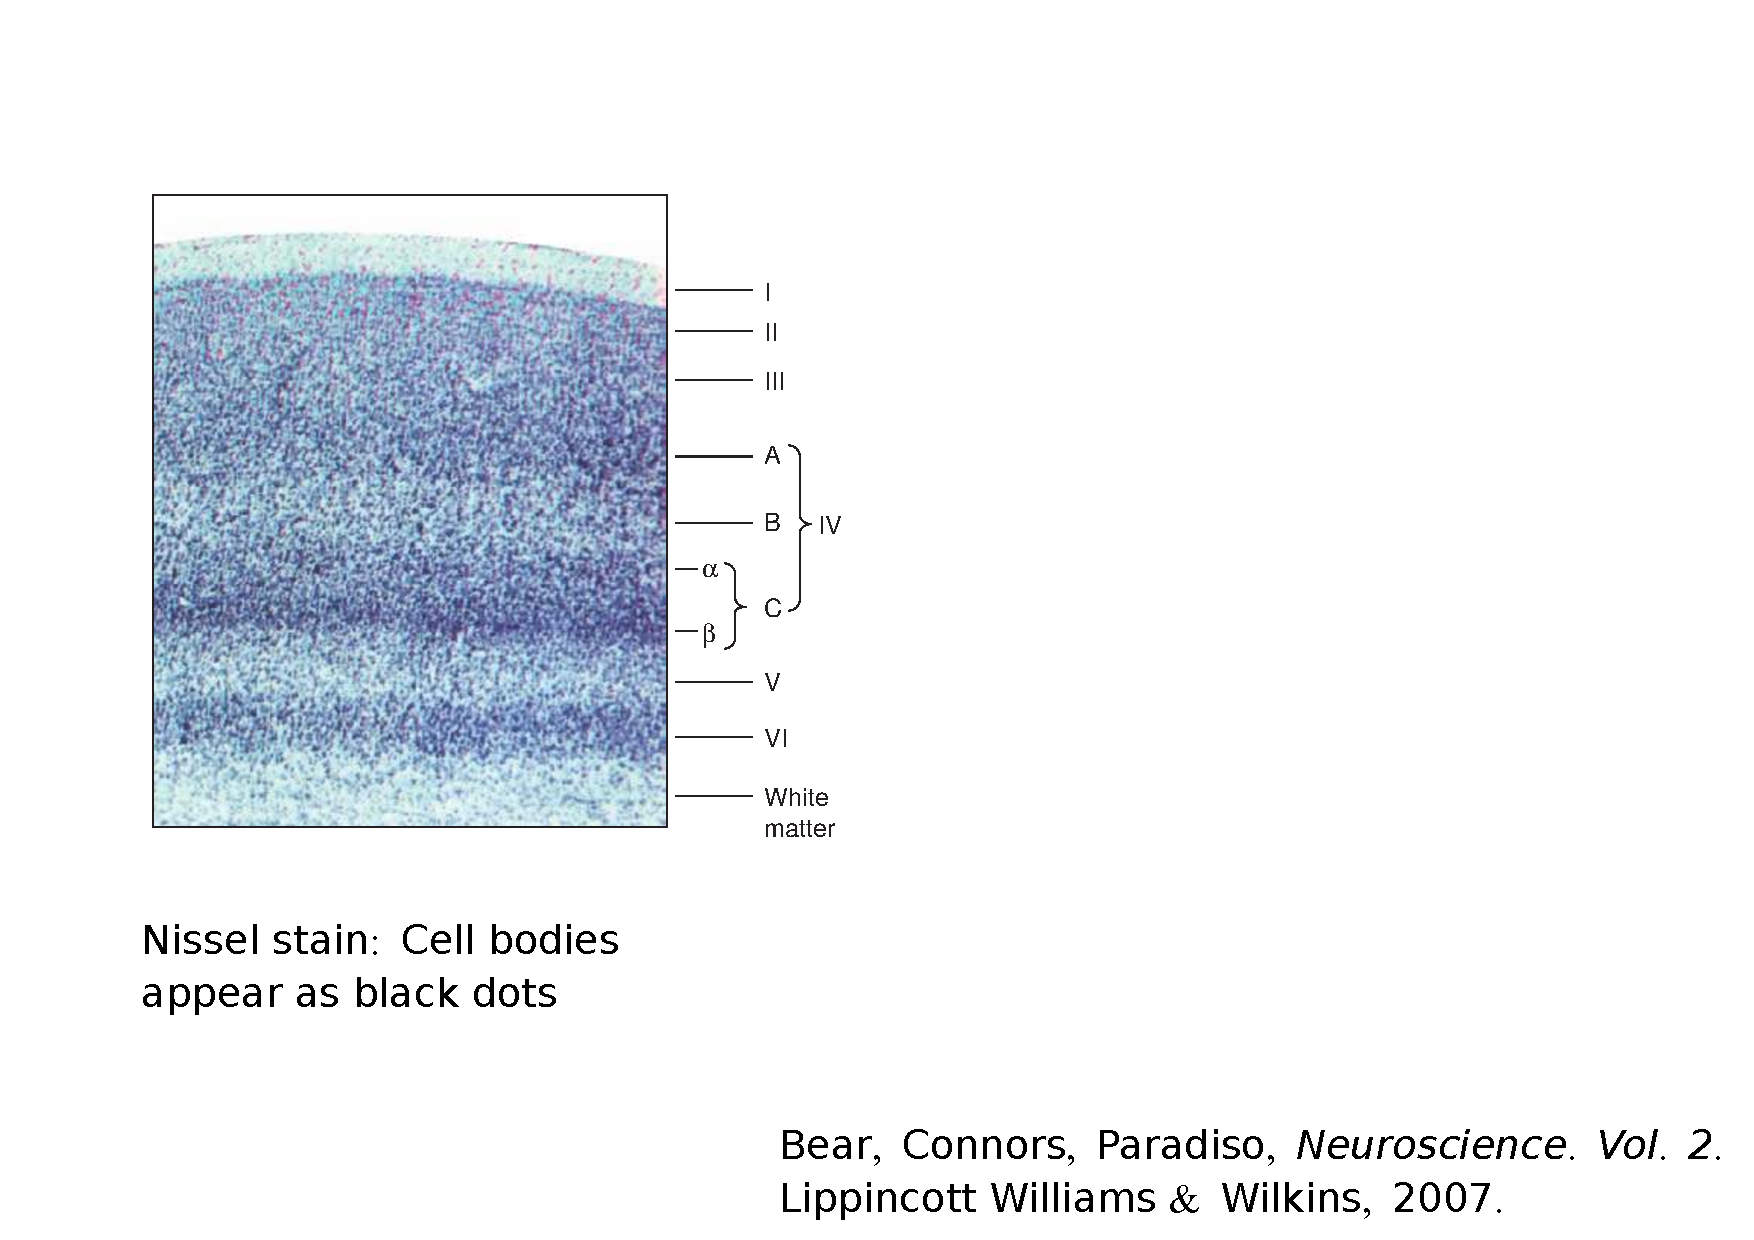
\includegraphics[height=0.9\textheight]{layers_pic1}
    }
    \only<2>{
    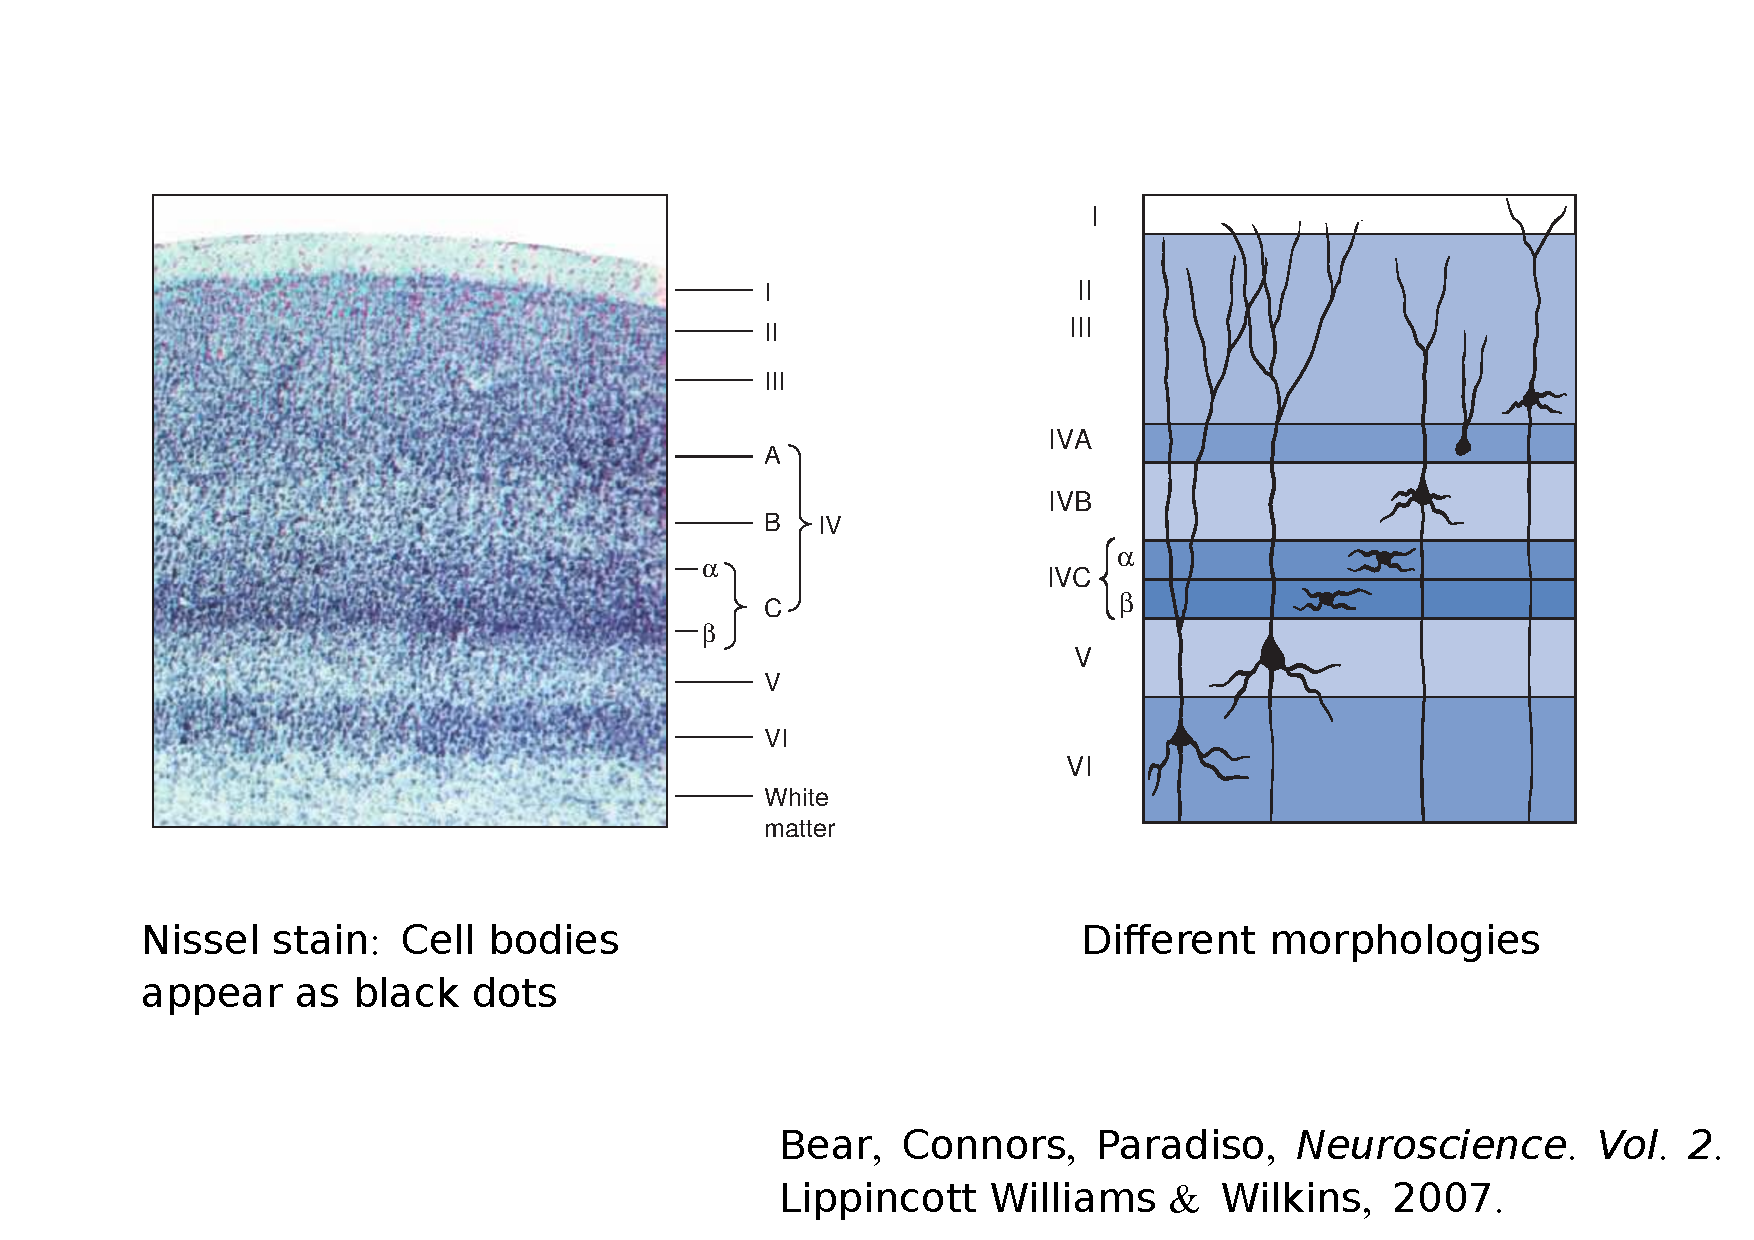
\includegraphics[height=0.9\textheight]{layers_pic2}
    }
\end{frame}

%%%%%%%%%%%%%%%%%%%%%%%%%%%%%%%%%%%%%%%%%%%%%%%%%%%%%%%%%%%%%
\section{Orientation Selectivity}
\label{sec:orientation_selectivity}

% Basics vision
\begin{frame}[t]{Vision}
    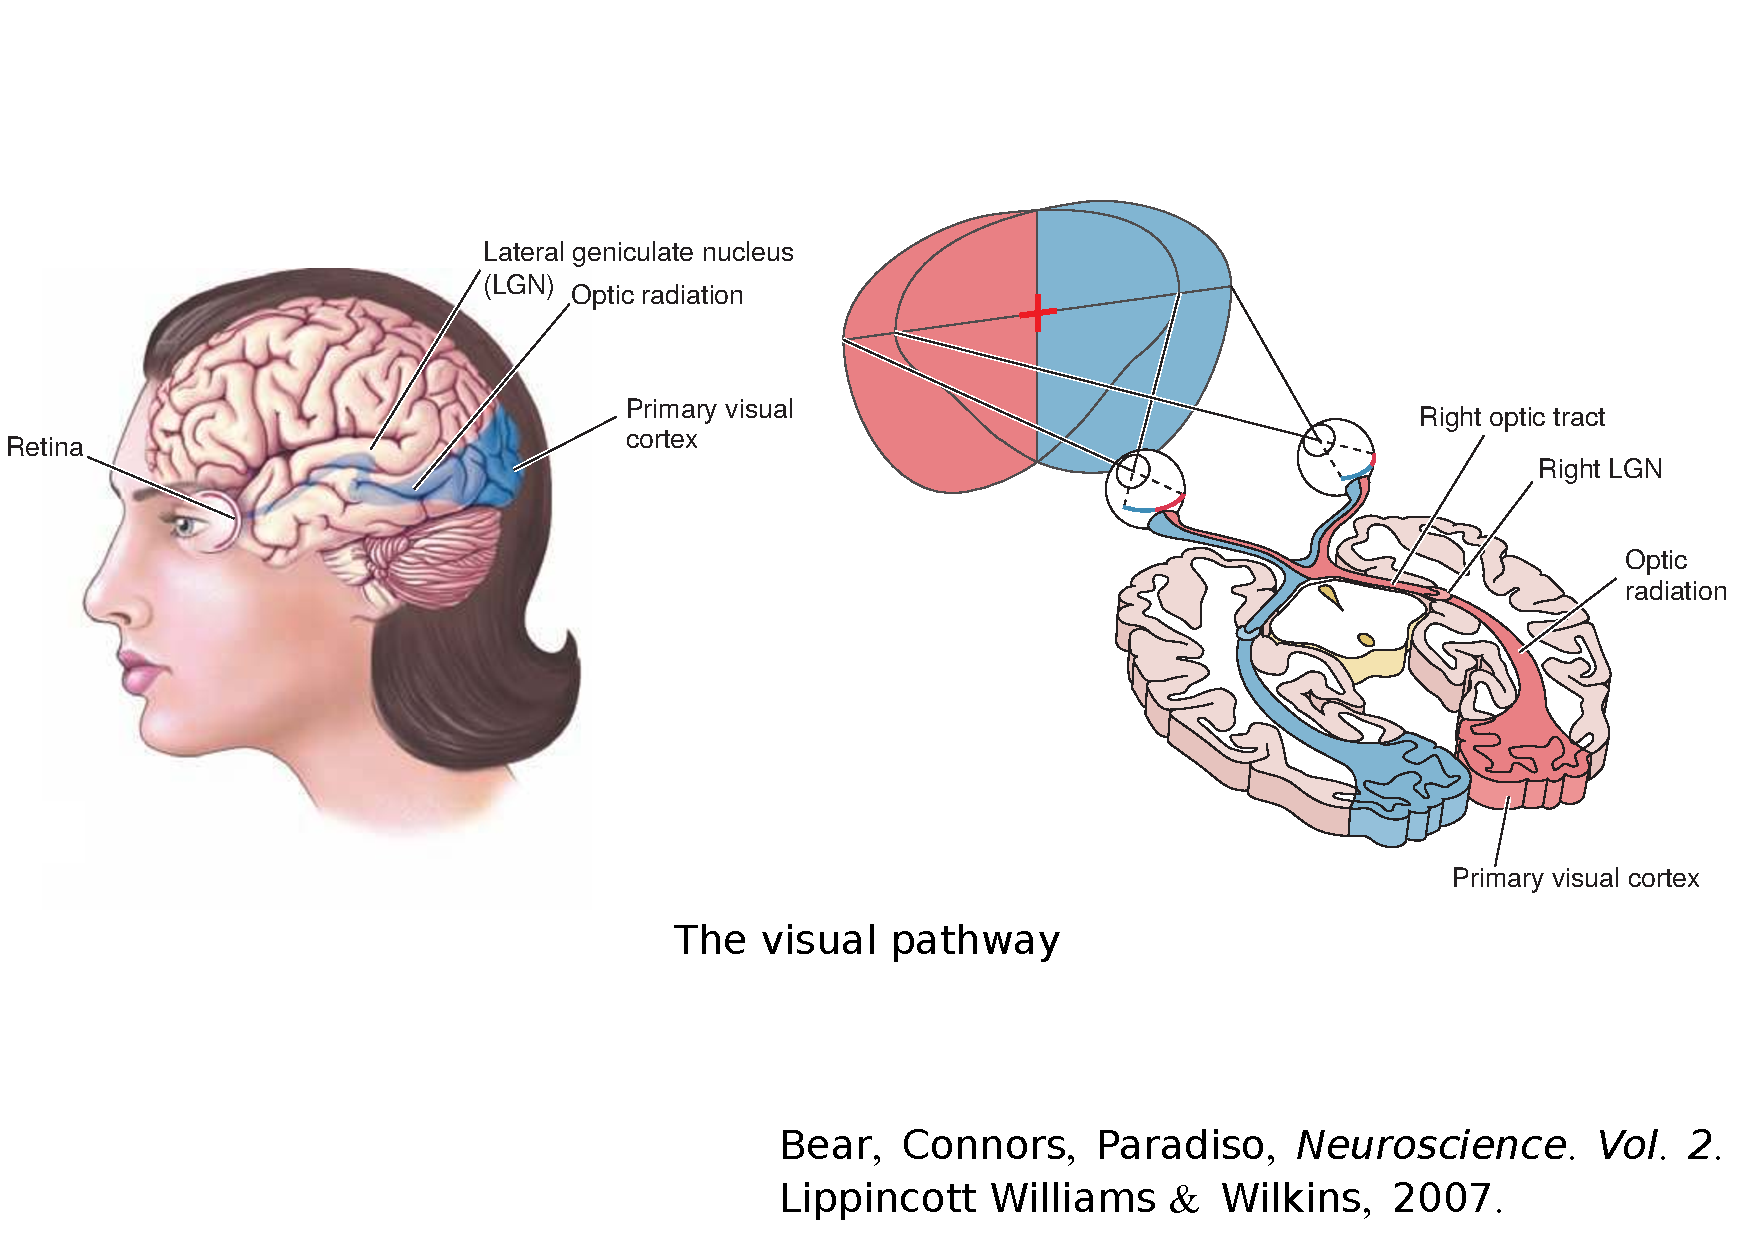
\includegraphics[height=0.9\textheight]{visual_pathway}
\end{frame}

% Hubel & Wiesel
\begin{frame}[t]{Hubel \& Wiesel 1959}
    \only<1>{
    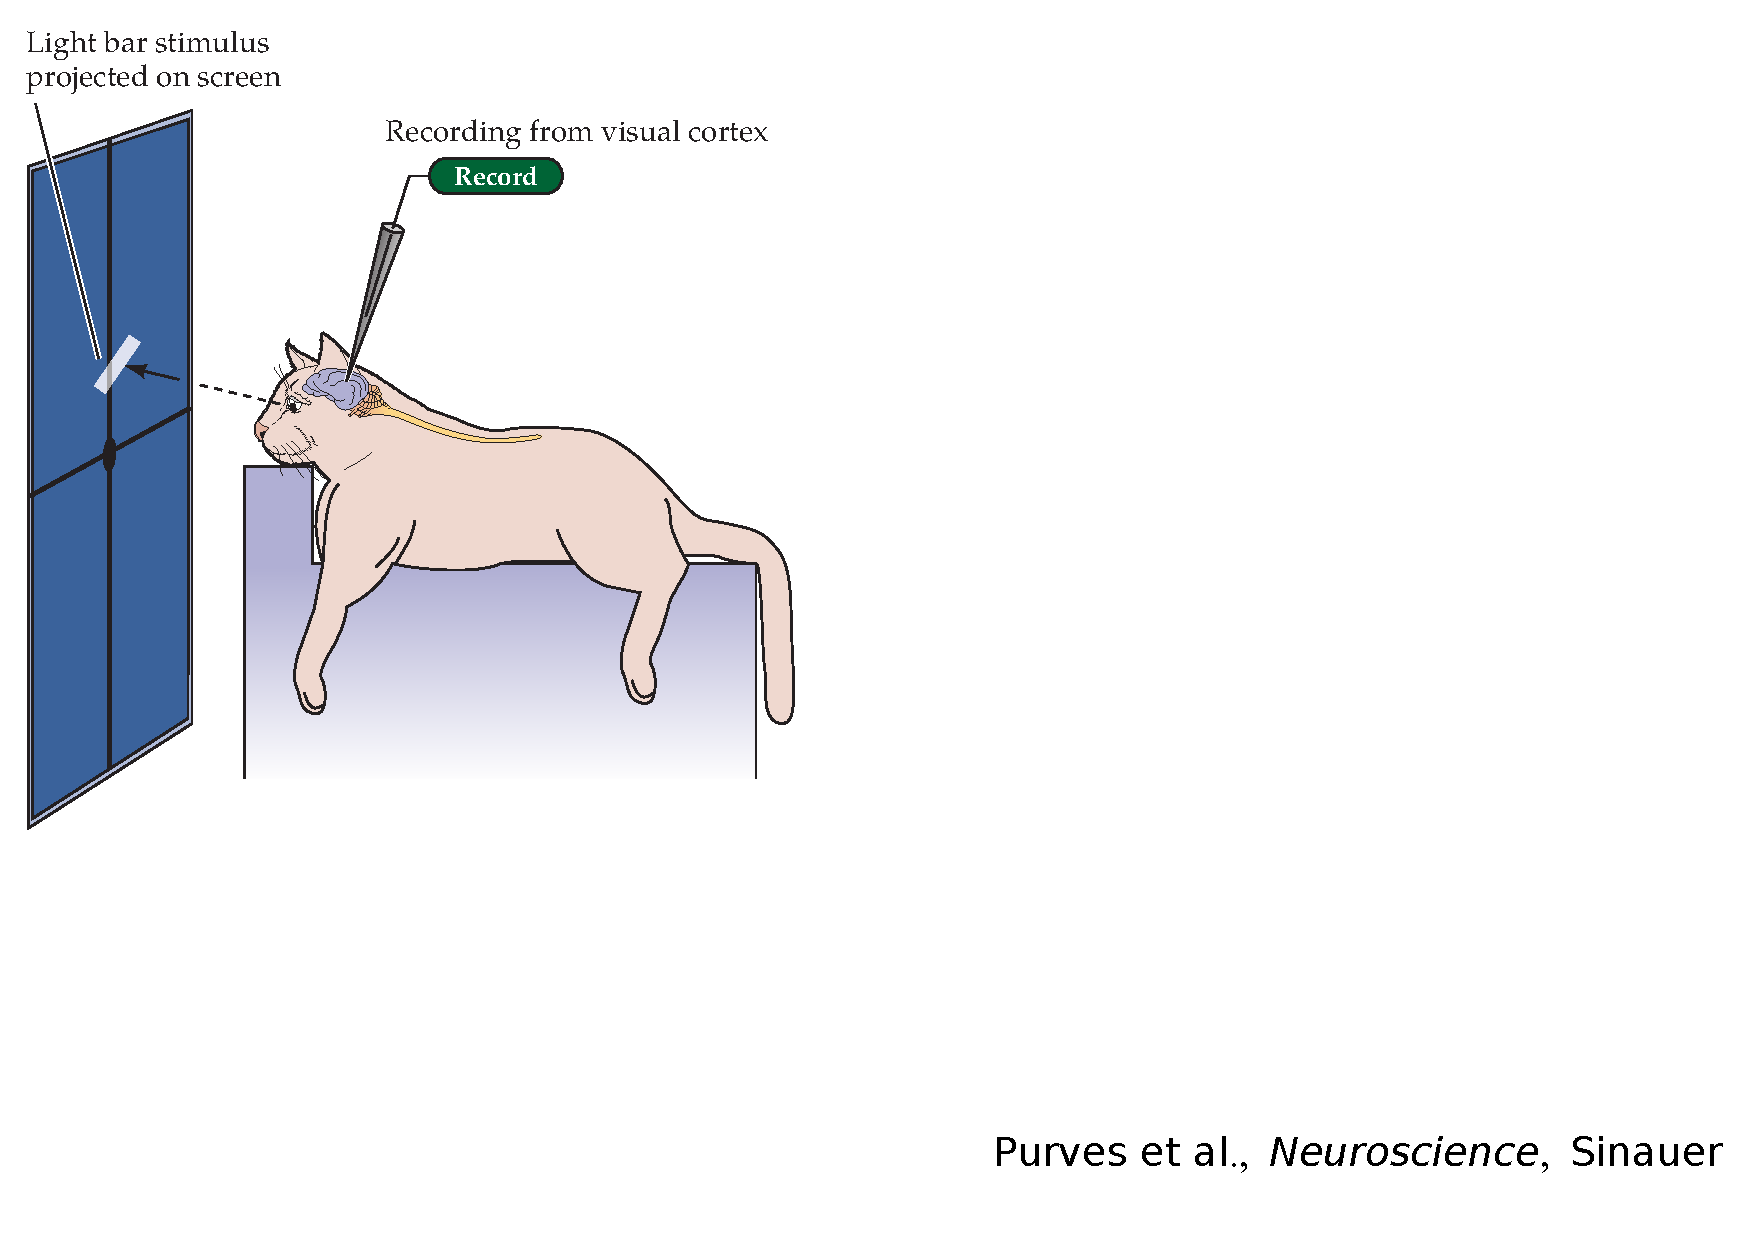
\includegraphics[height=0.9\textheight]{hubel_wiesel1}
    }
    \only<2>{
    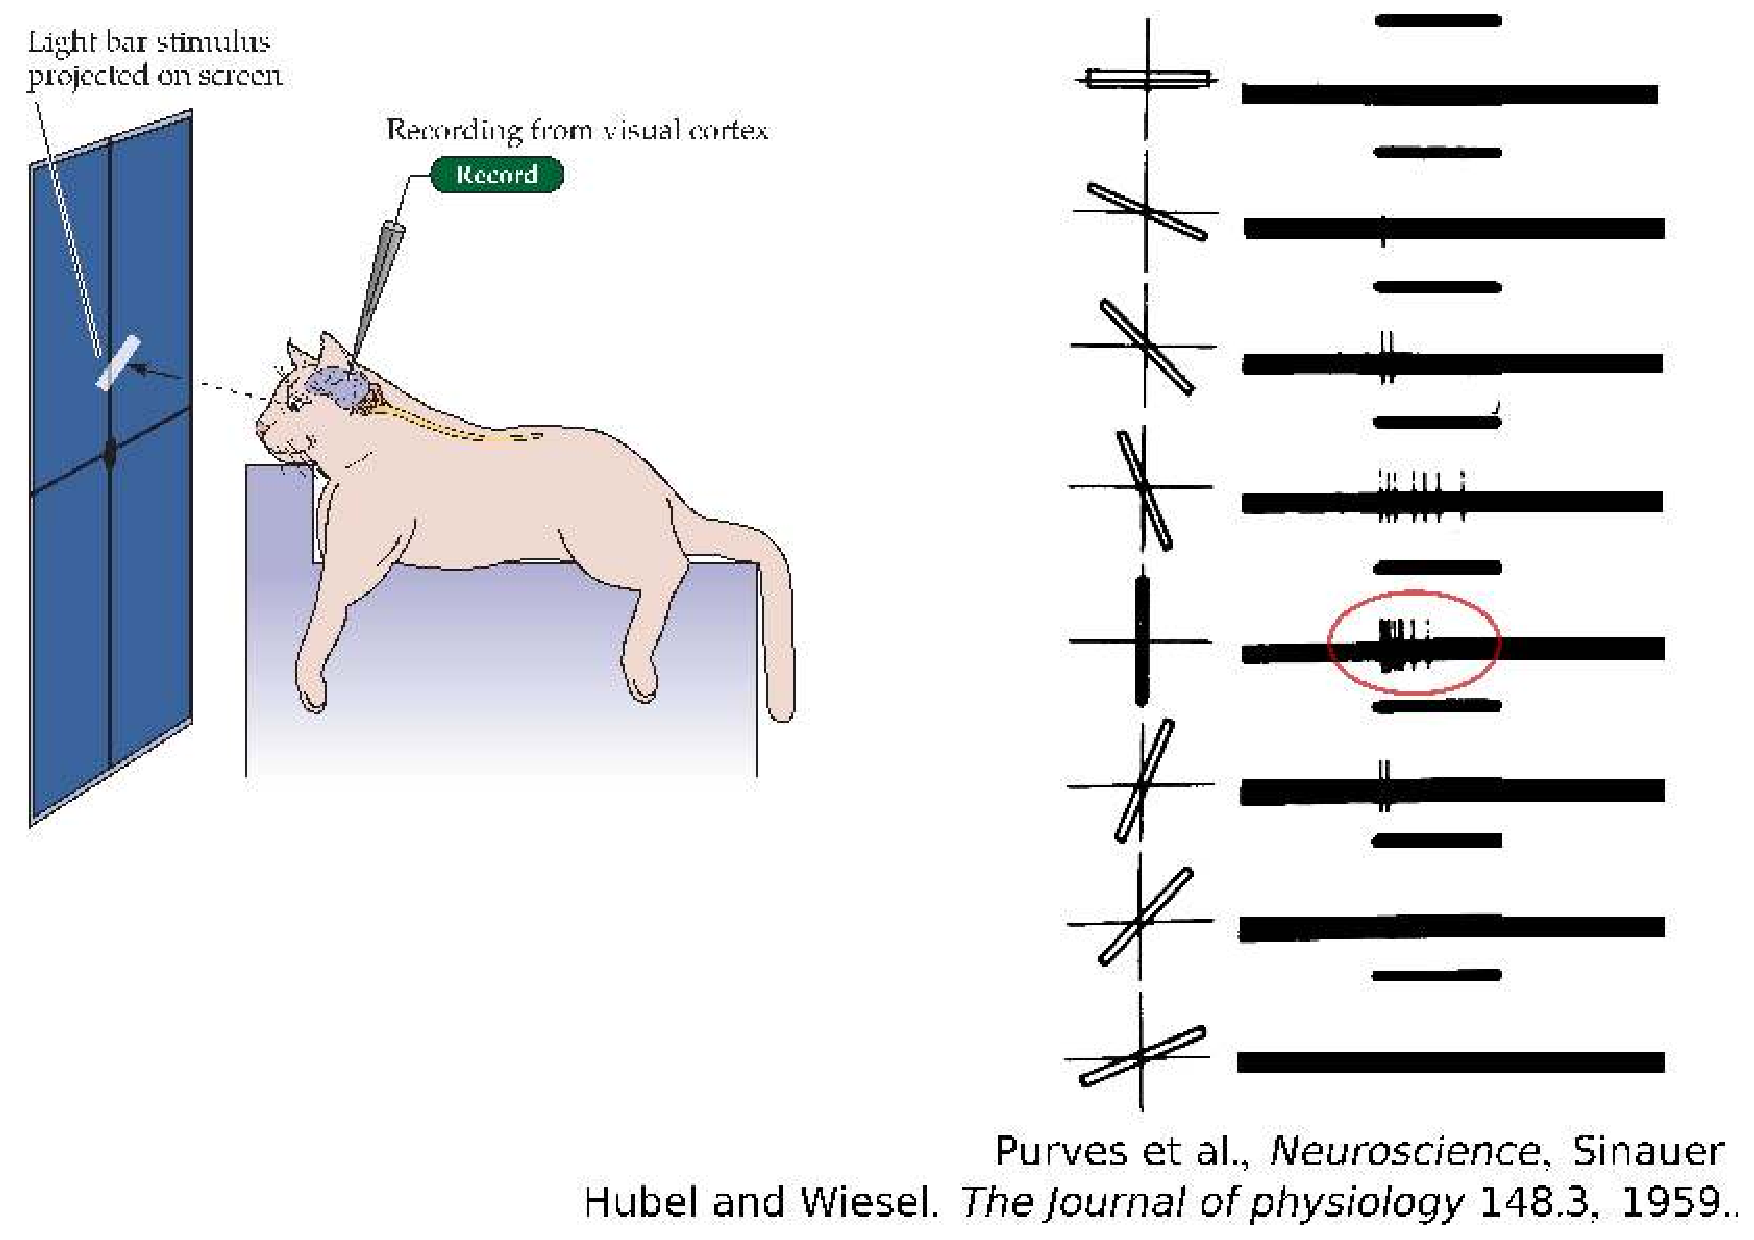
\includegraphics[height=0.9\textheight]{hubel_wiesel2}
    }
    \only<3>{
    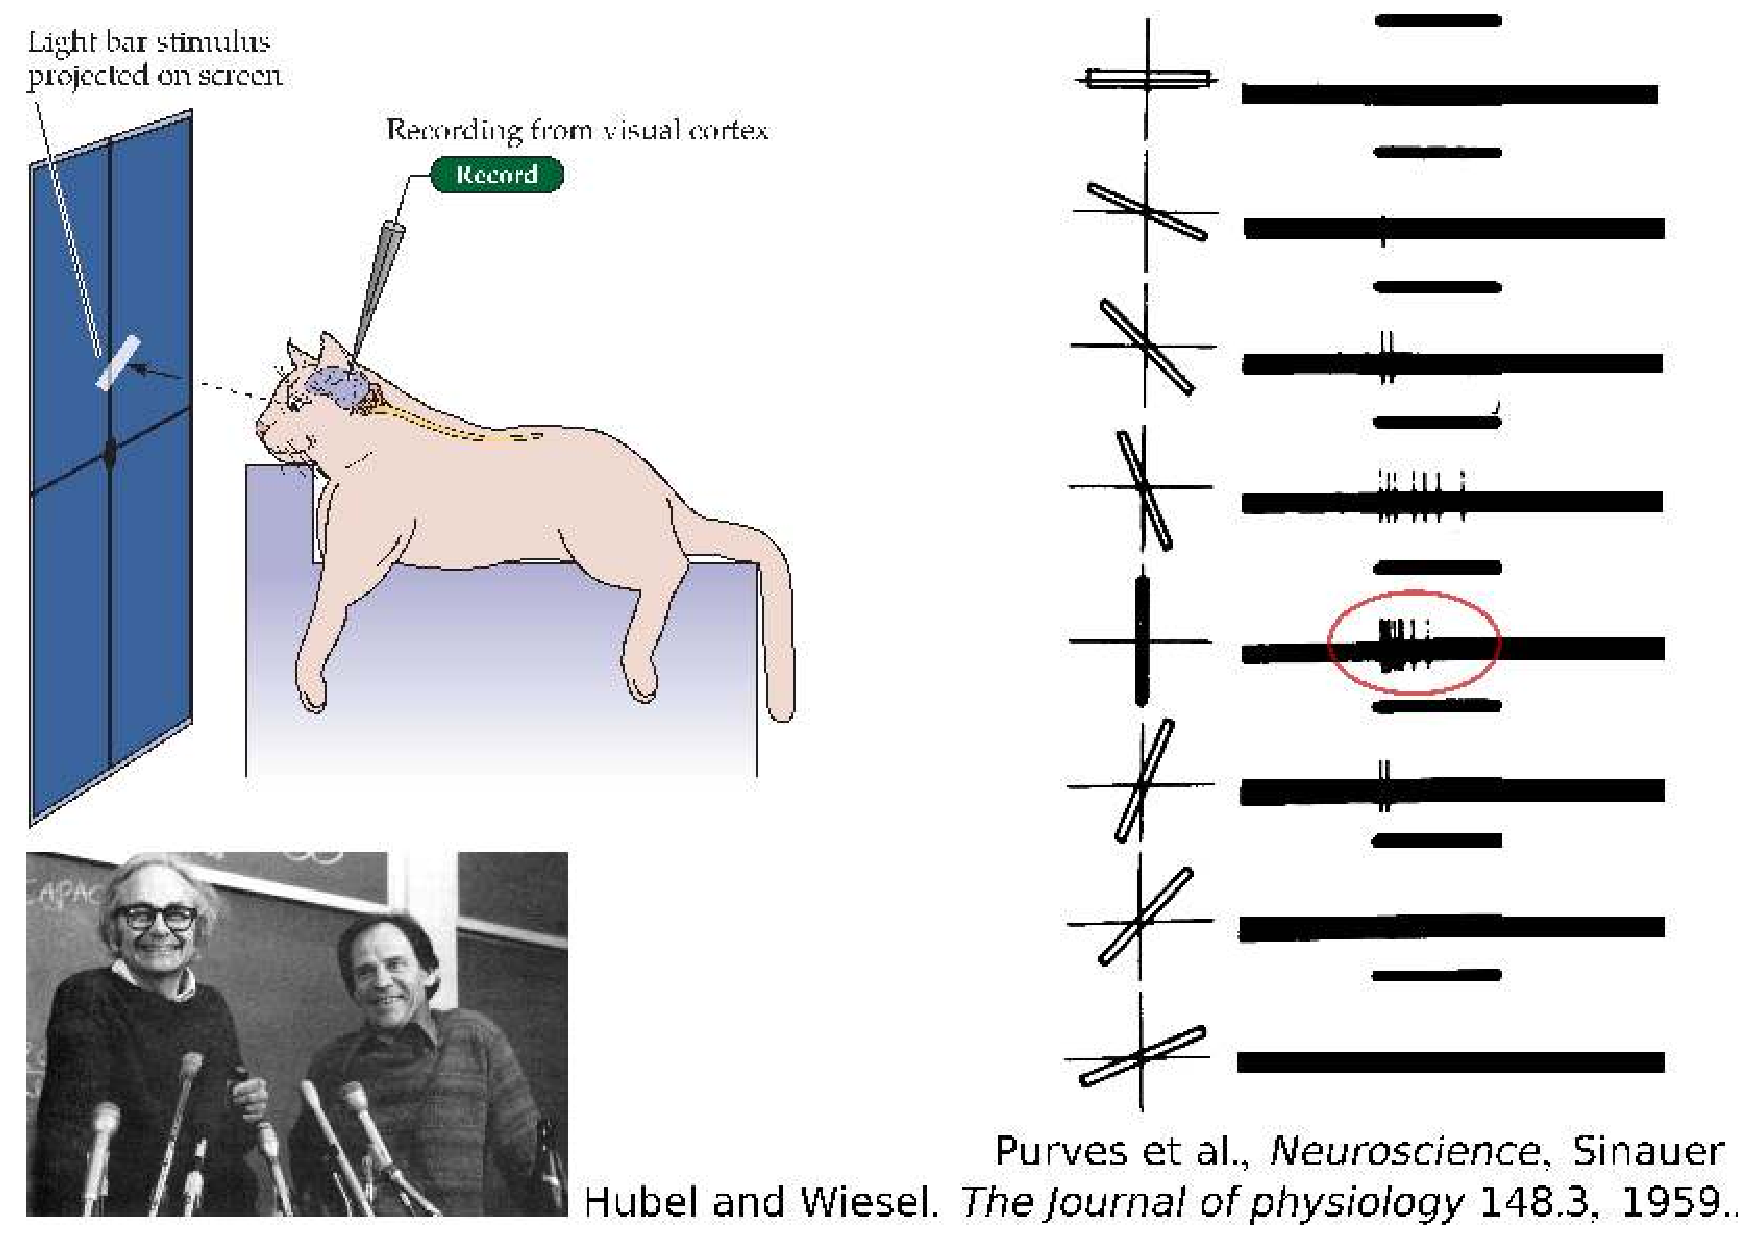
\includegraphics[height=0.9\textheight]{hubel_wiesel}
    }
\end{frame}

% Tuning curves
\begin{frame}[t]{Tuning curves}
    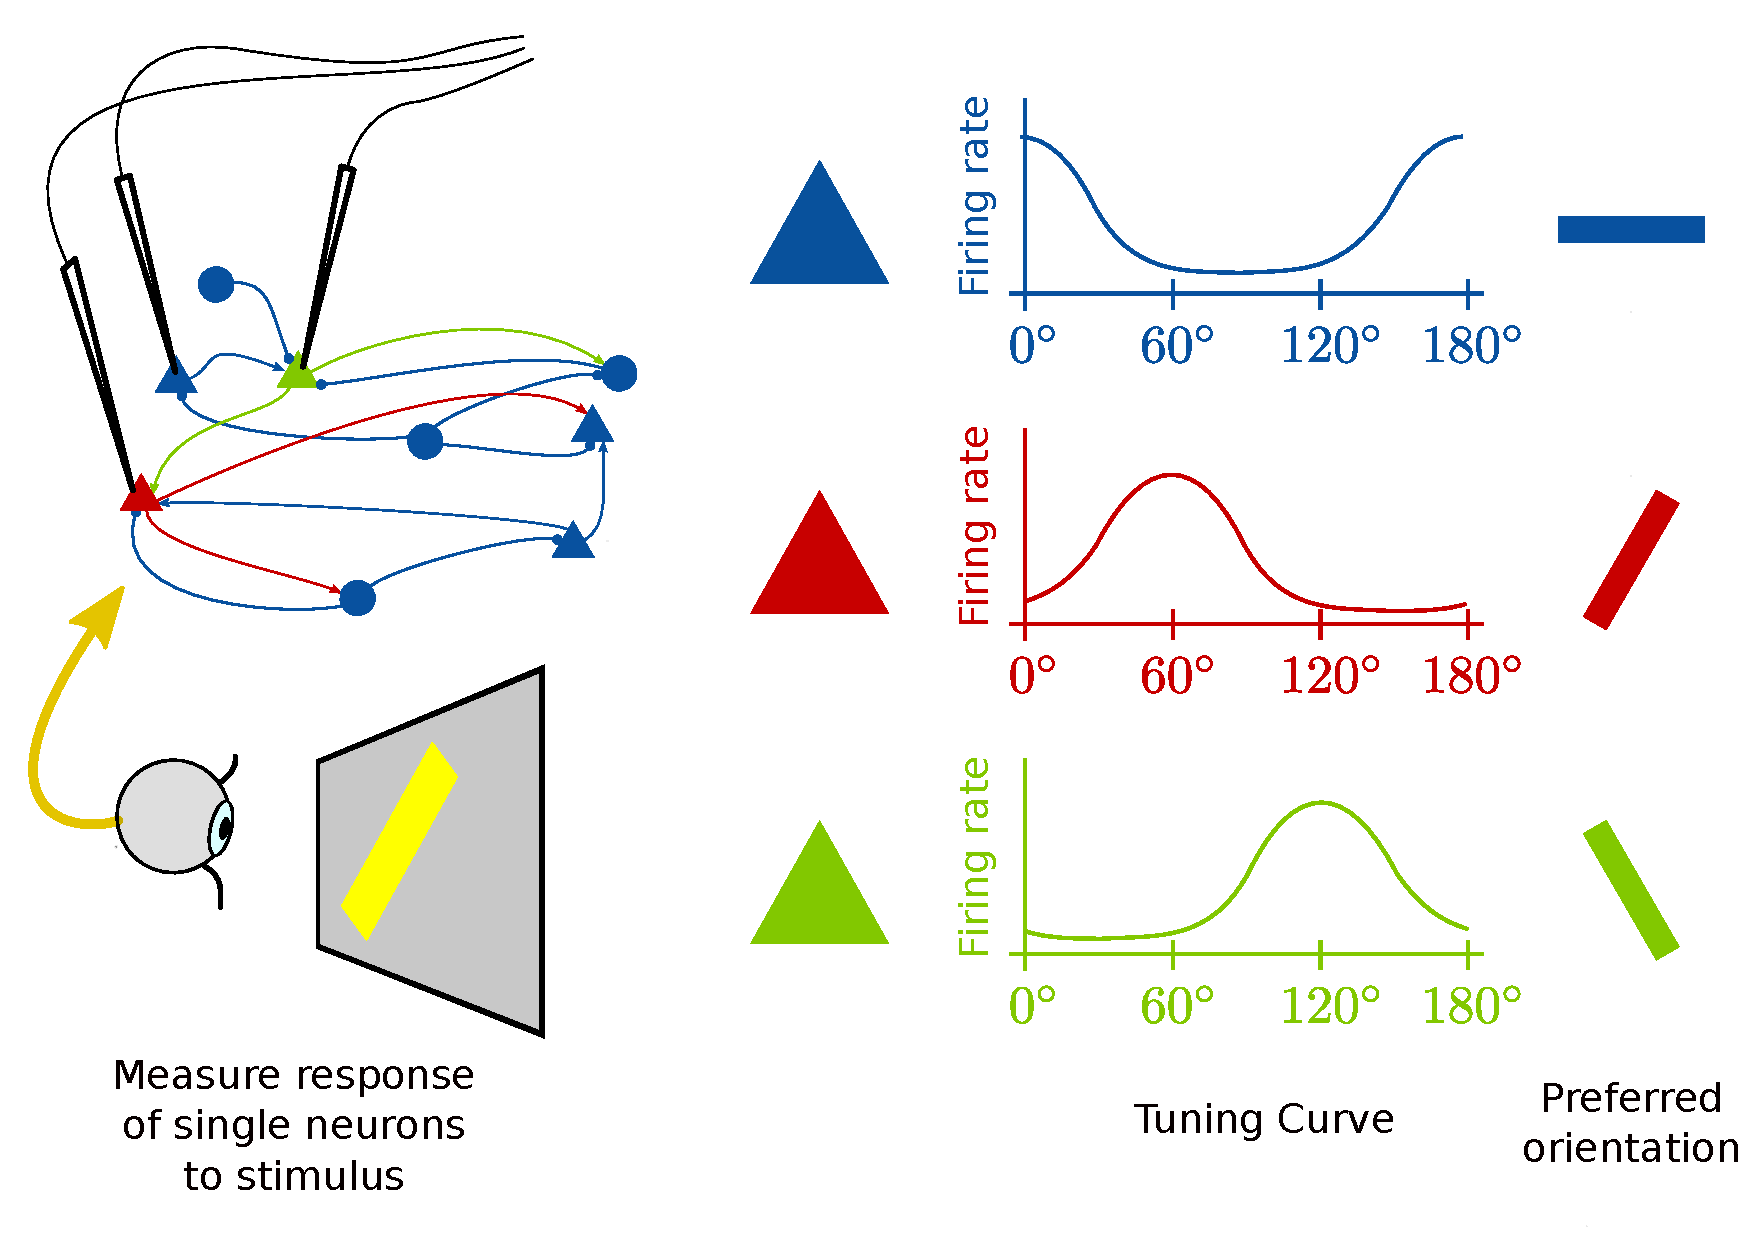
\includegraphics[height=0.9\textheight]{tuning_curves}
\end{frame}


\section{Emergence of functional specificity}
\label{sec:emergence_of_functional_microcircuits}

% Idea
\begin{frame}[t]{Basic idea}
    \only<1>{
    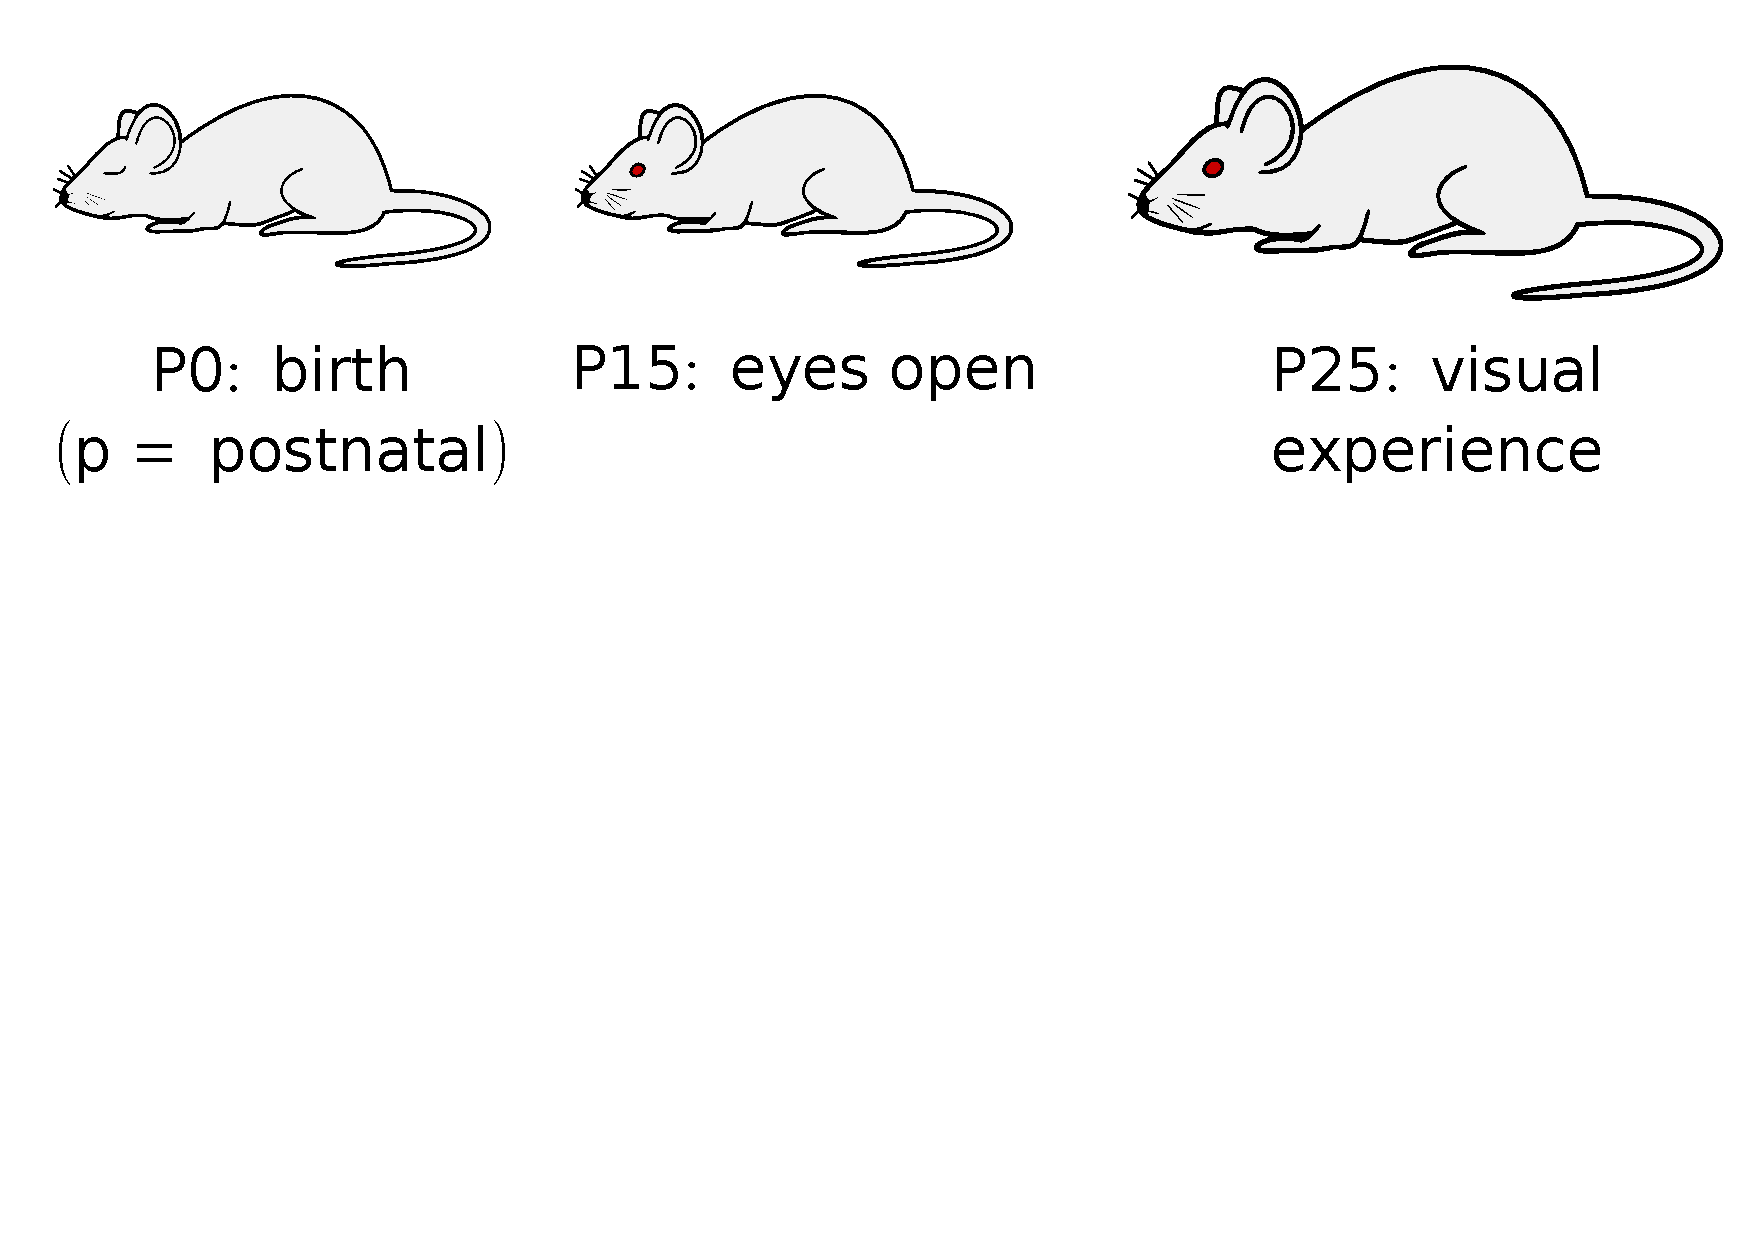
\includegraphics[height=0.9\textheight]{mouse_scheme1}
    }
    \only<2>{
    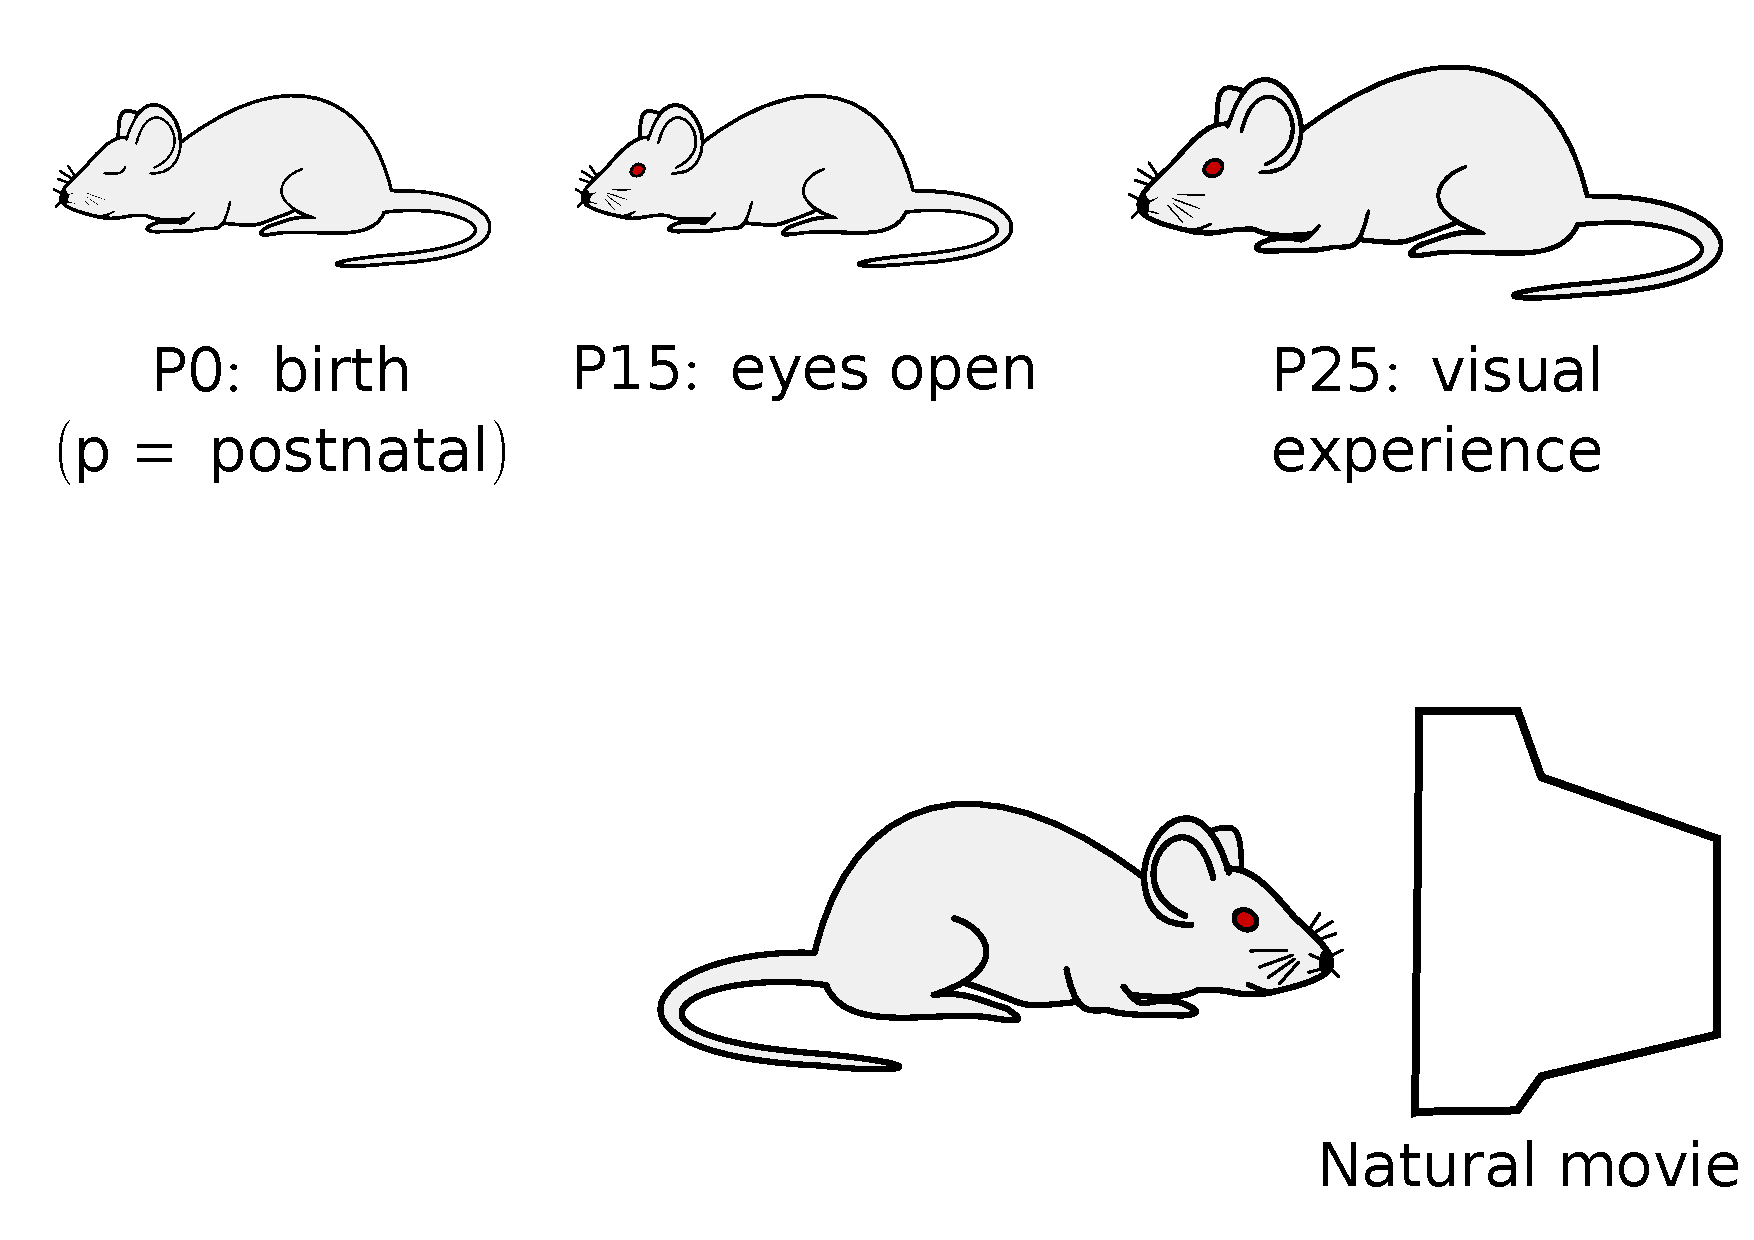
\includegraphics[height=0.9\textheight]{mouse_scheme2}
    }
    \only<3>{
    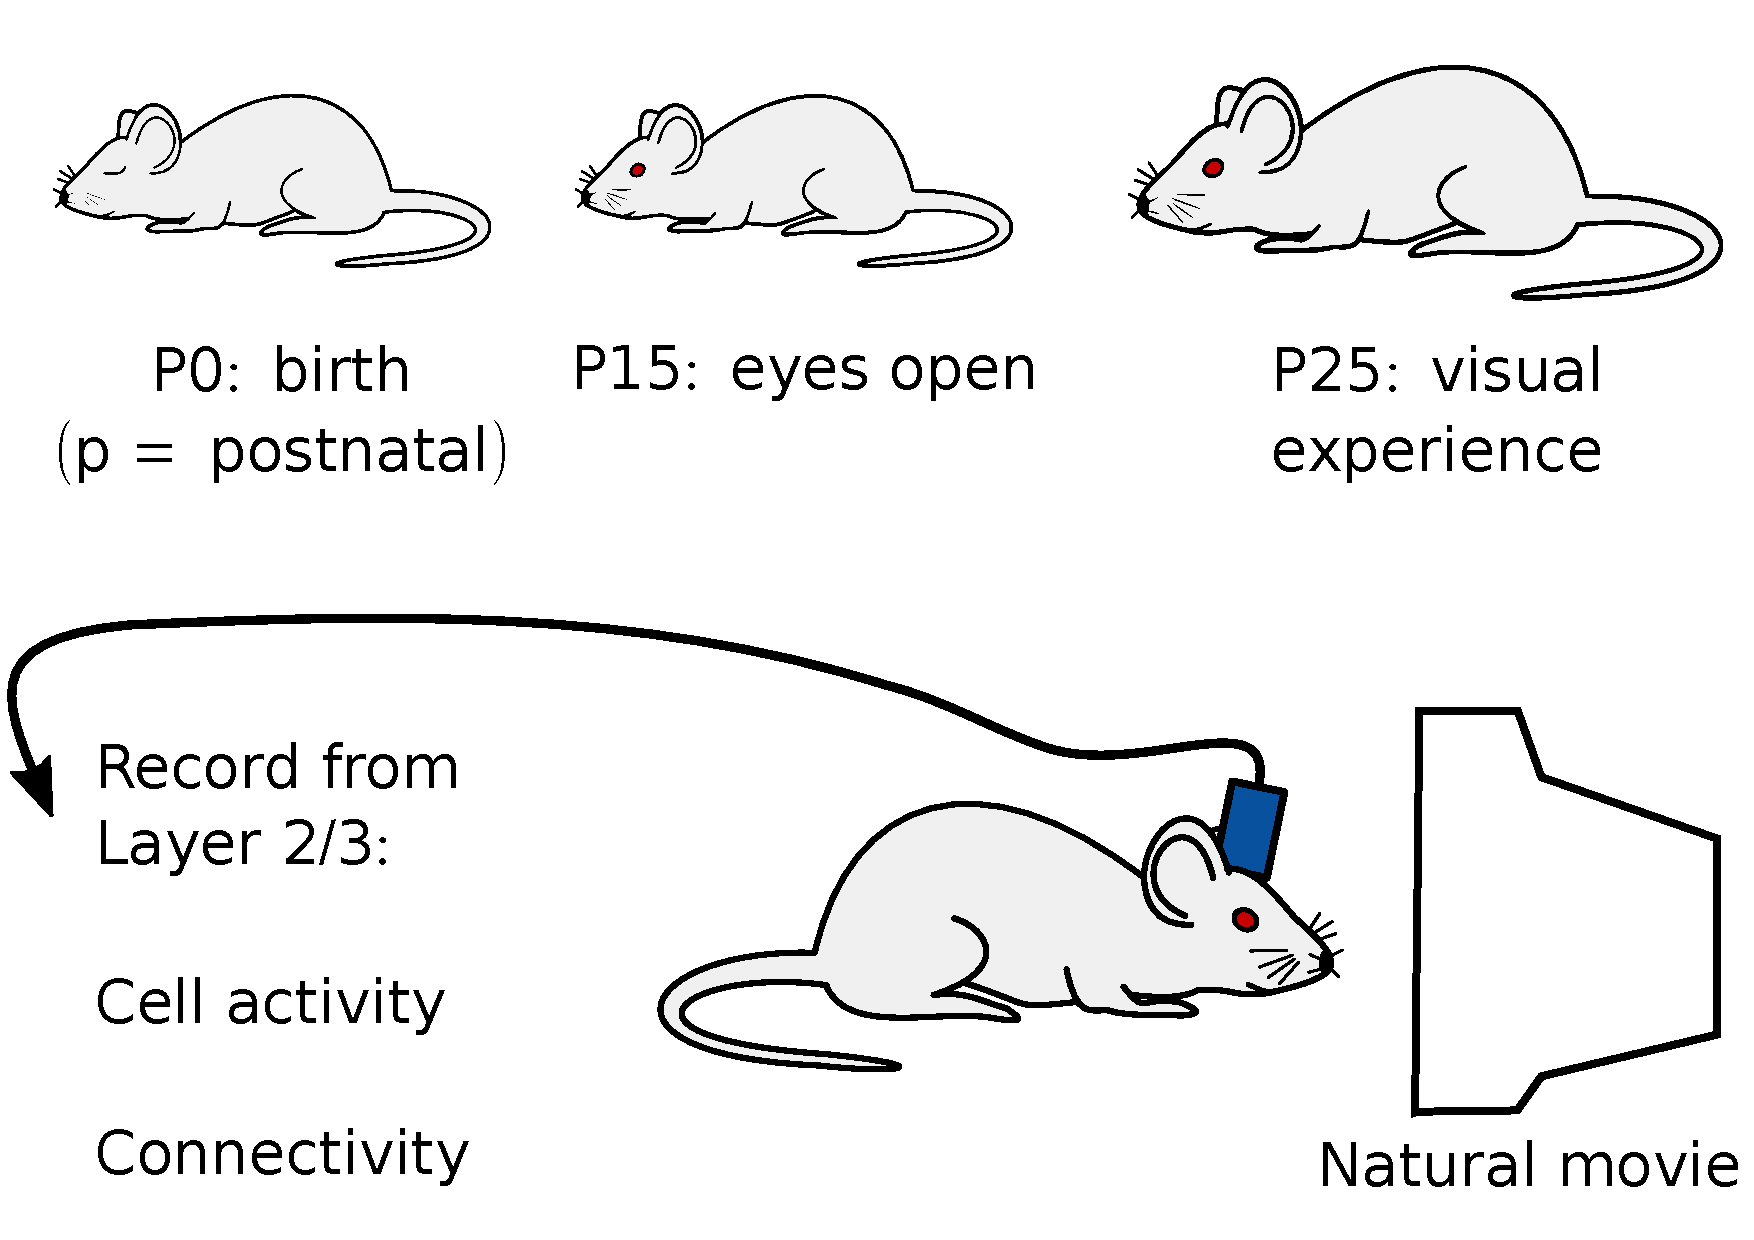
\includegraphics[height=0.9\textheight]{mouse_scheme}
    }
\end{frame}

% Experimental results
\begin{frame}[t]{Two-photon calcium imaging}
    \only<1>{
    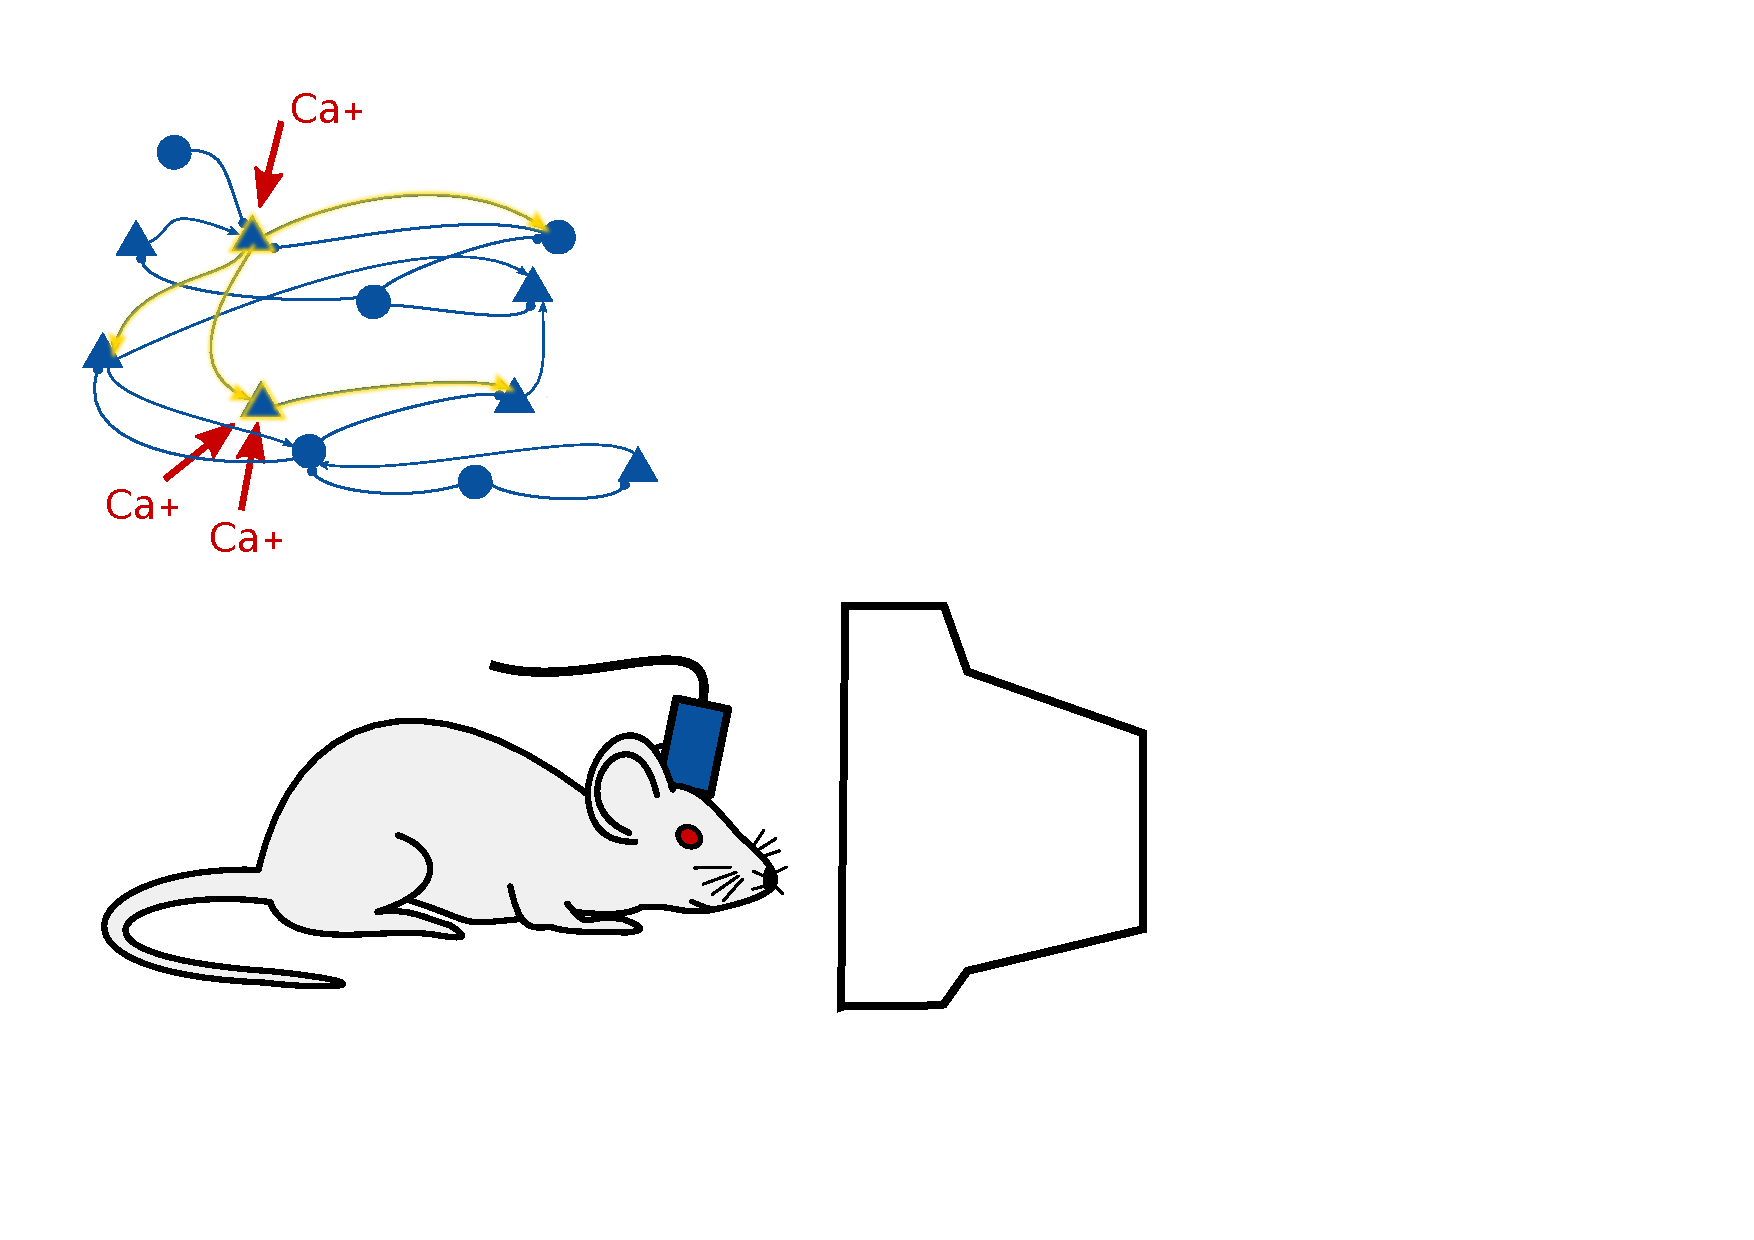
\includegraphics[height=0.9\textheight]{calcium_imaging1}
    }
    \only<2>{
    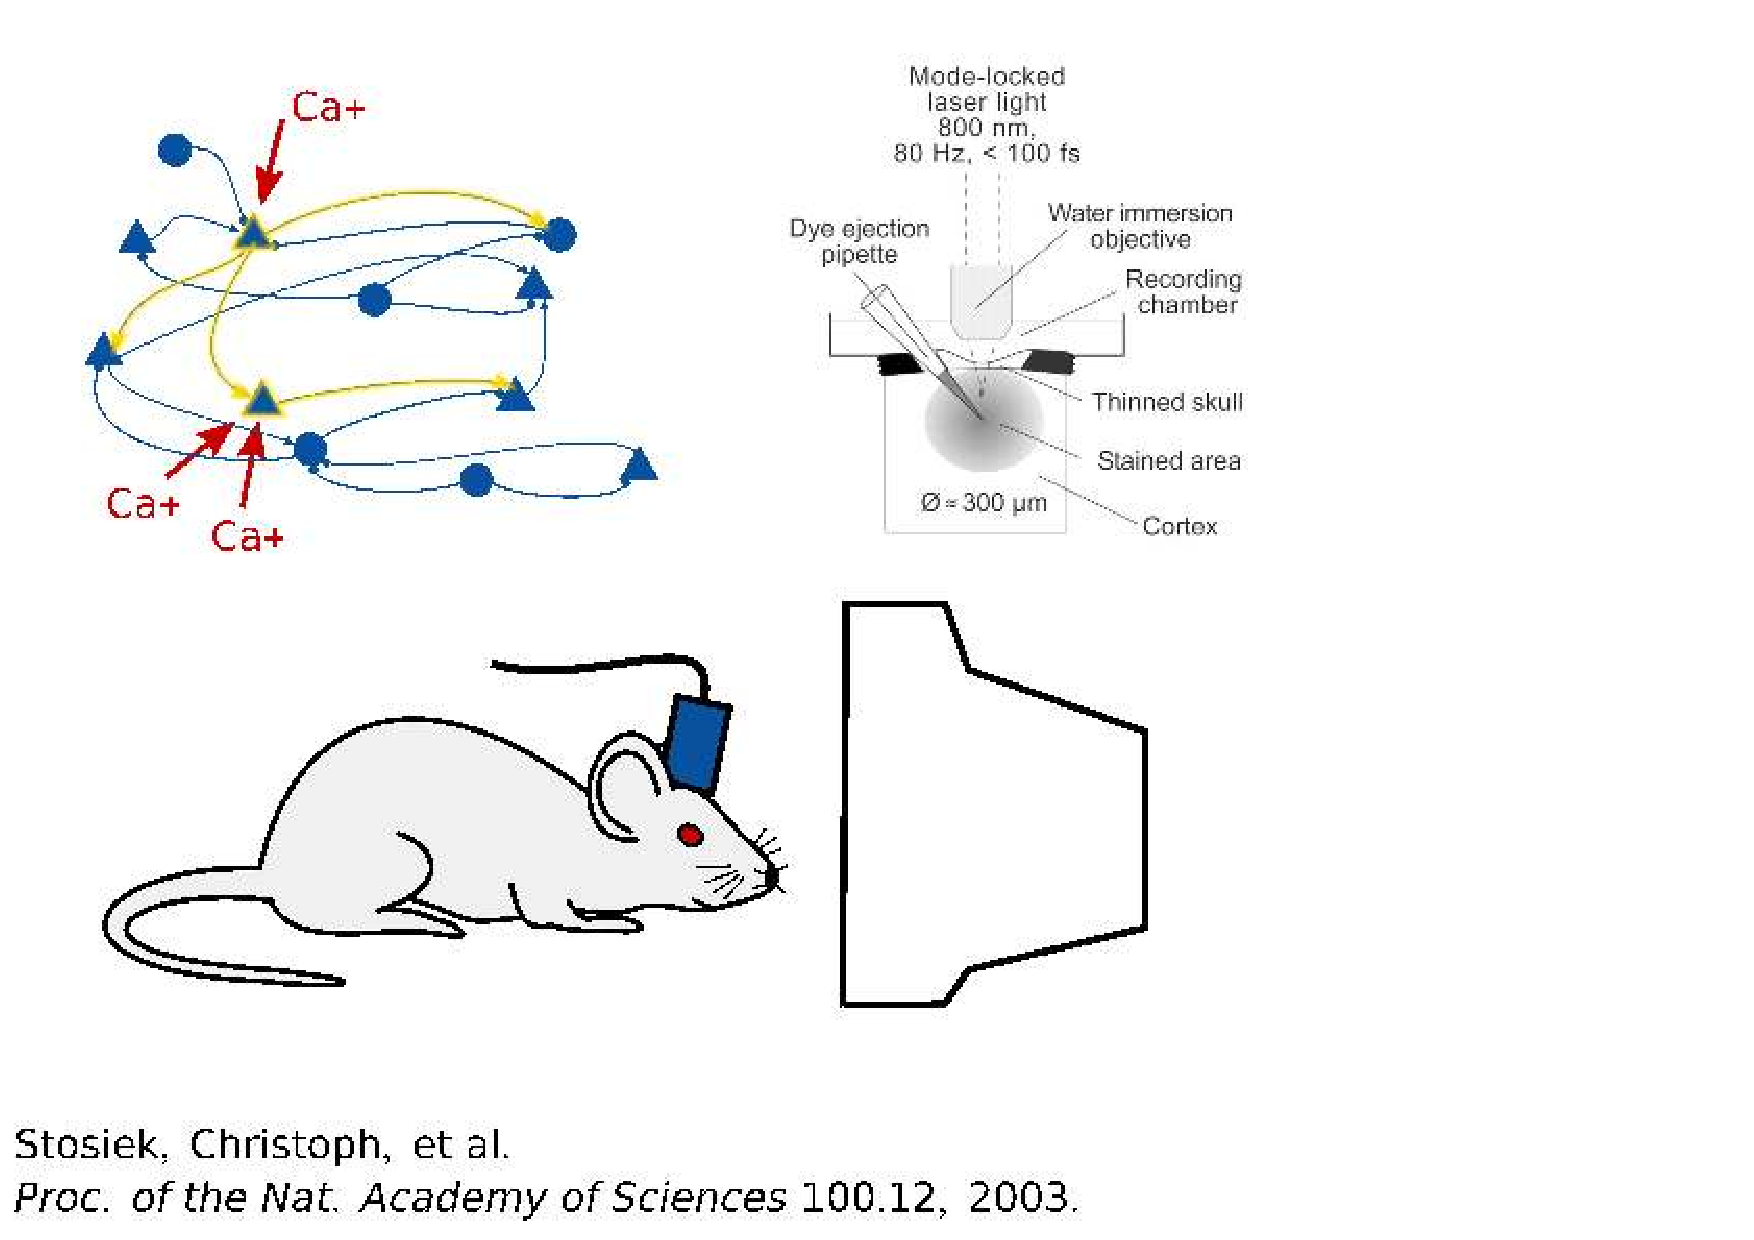
\includegraphics[height=0.9\textheight]{calcium_imaging2}
    }
    \only<3>{
    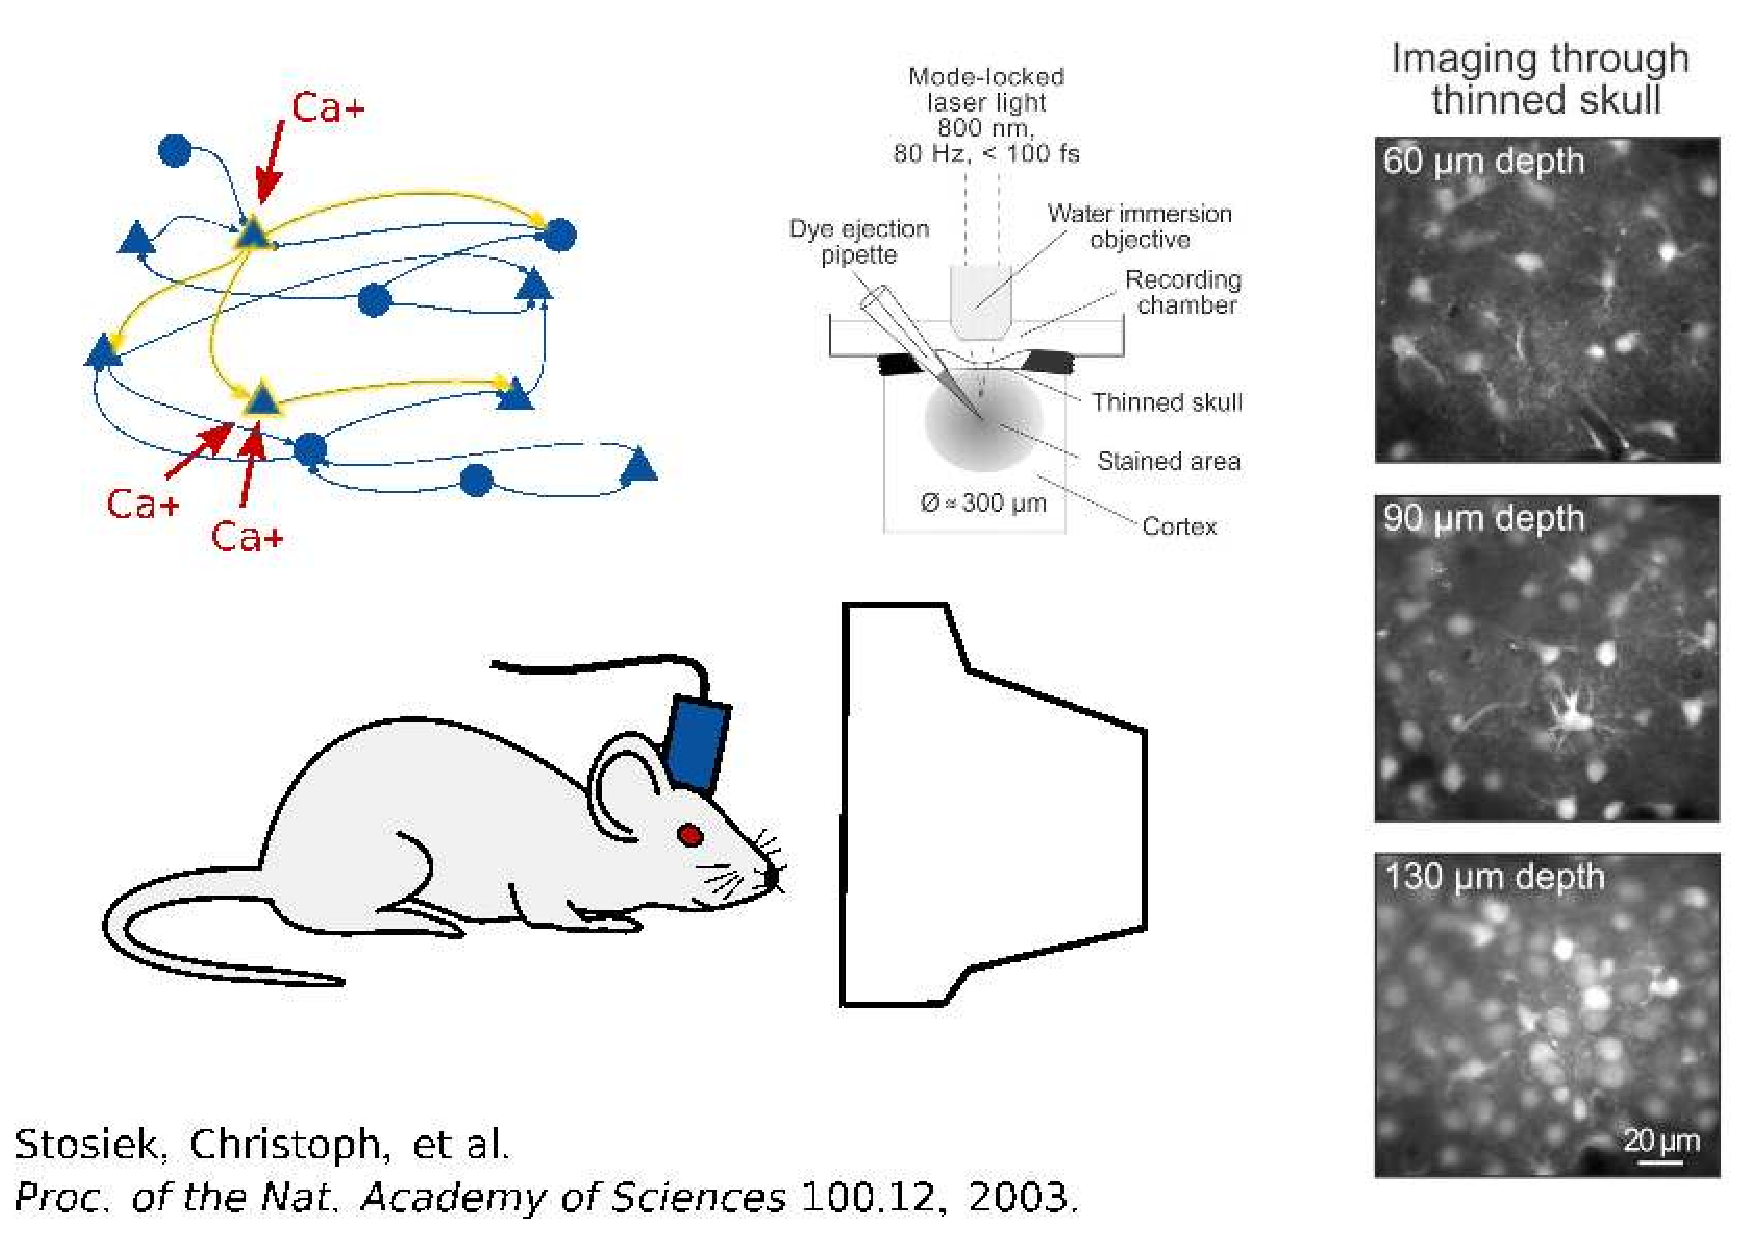
\includegraphics[height=0.9\textheight]{calcium_imaging}
    }
\end{frame}

%Receptive fields
\begin{frame}[t]{Receptive fields}
    \only<1>{
    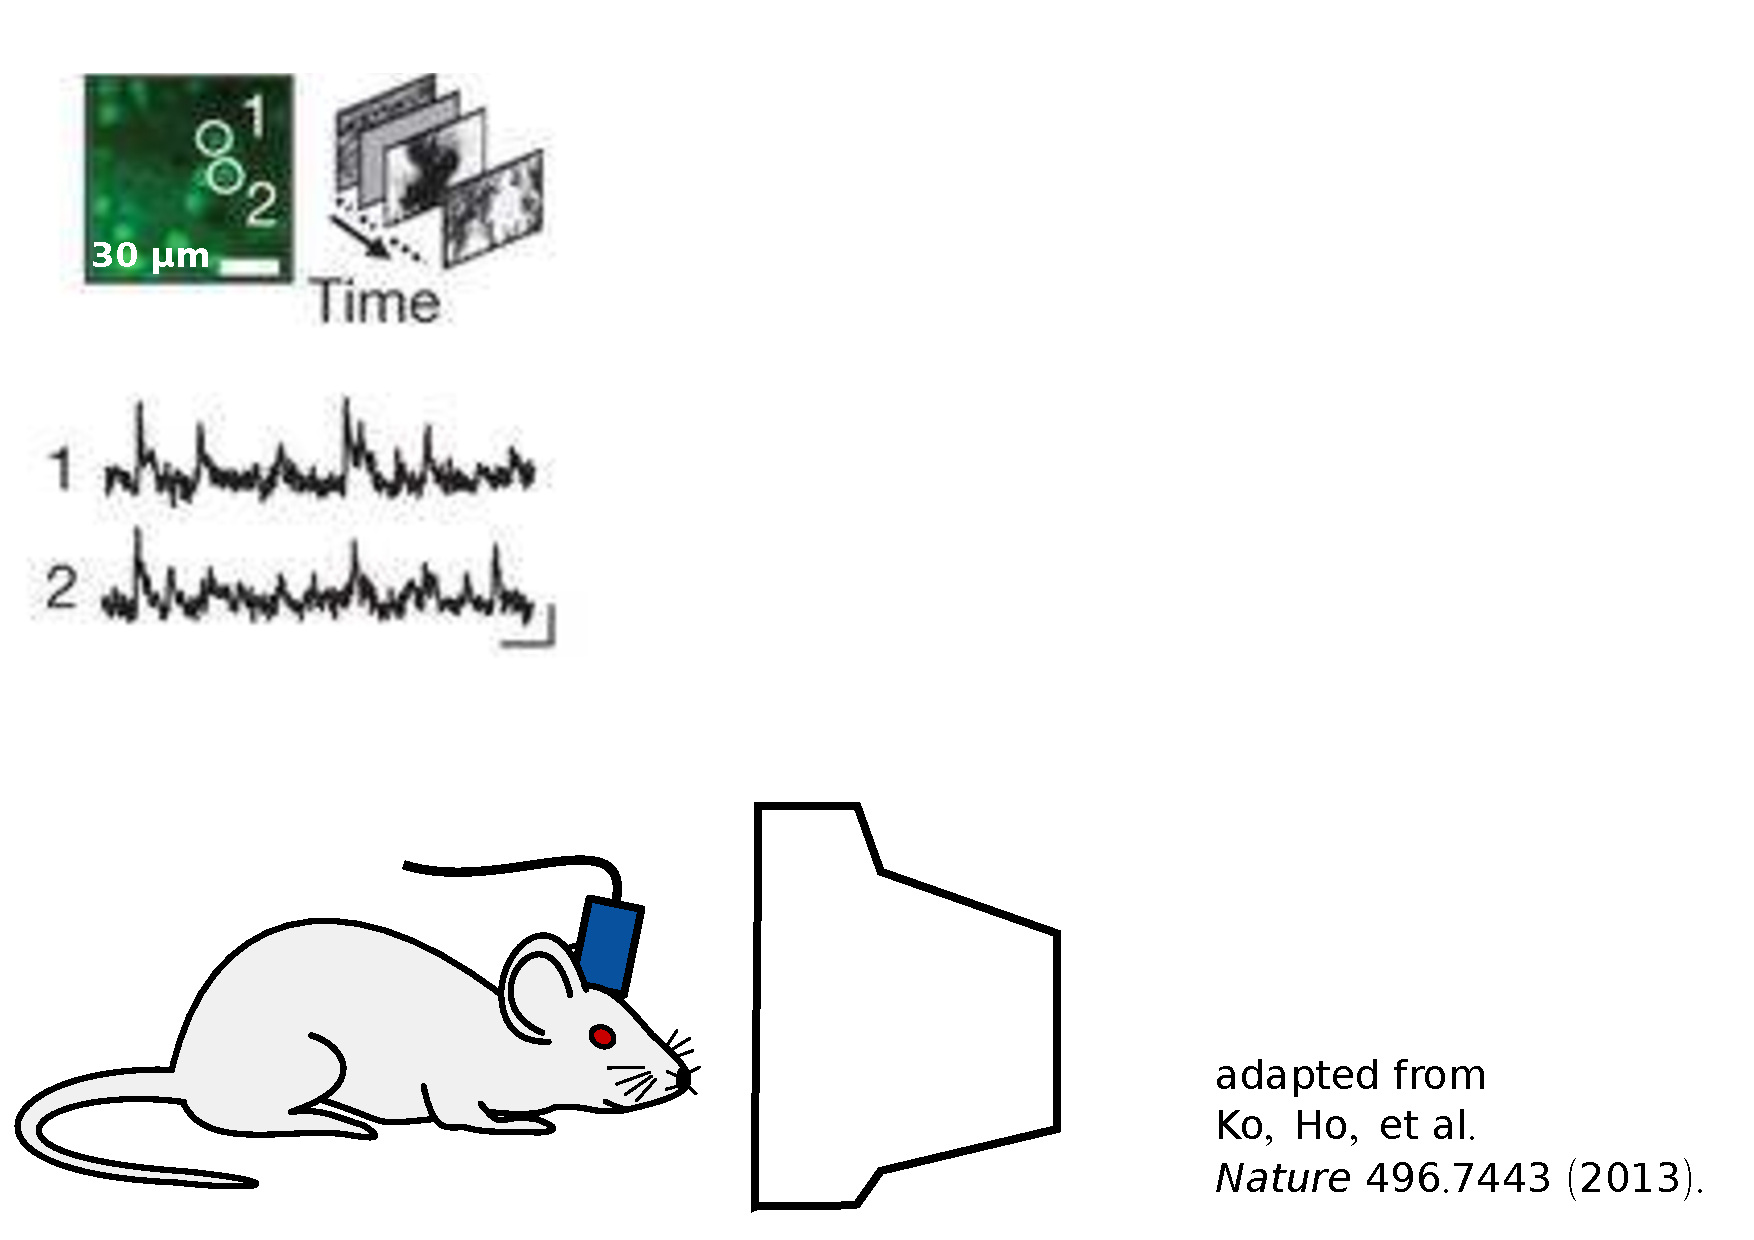
\includegraphics[height=0.9\textheight]{ko_rfs1}
    }
    \only<2>{
    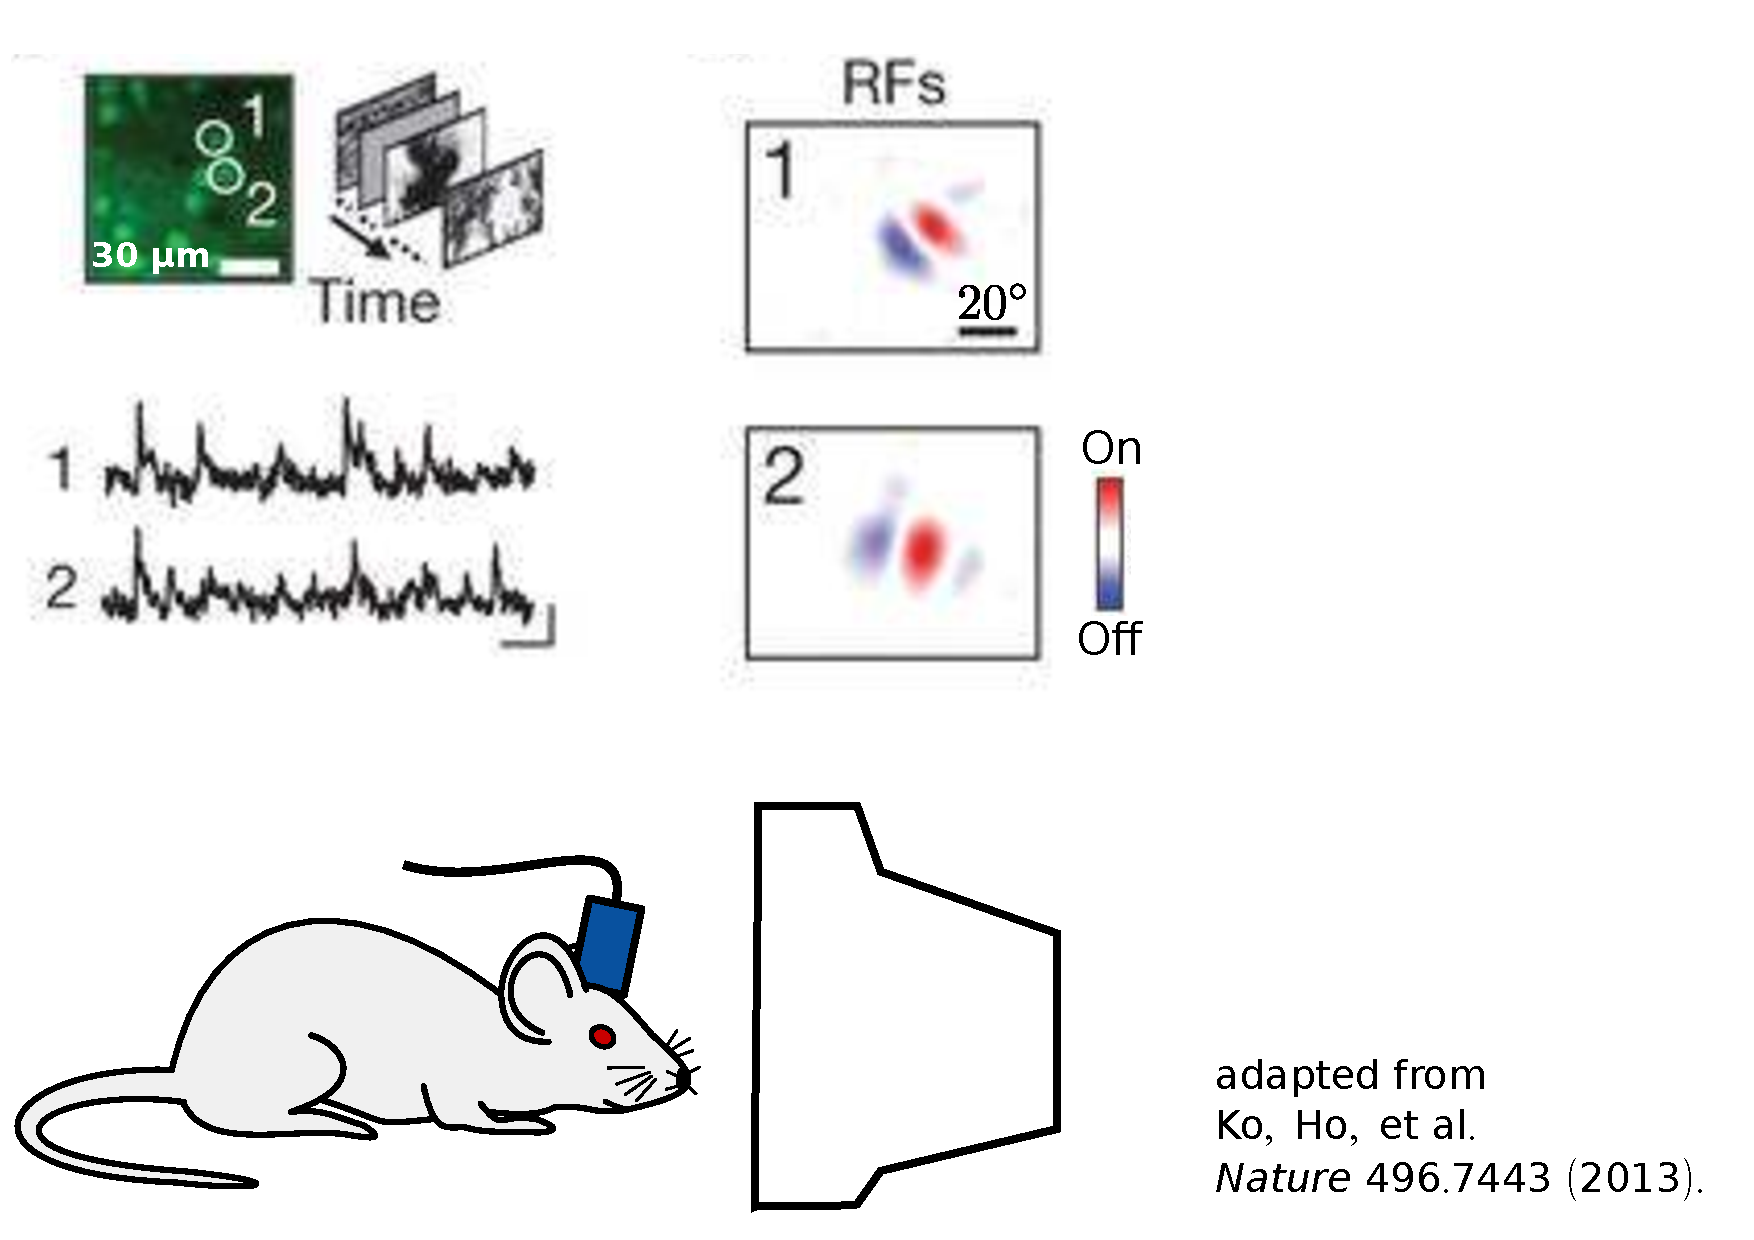
\includegraphics[height=0.9\textheight]{ko_rfs2}
    }
    \only<3>{
    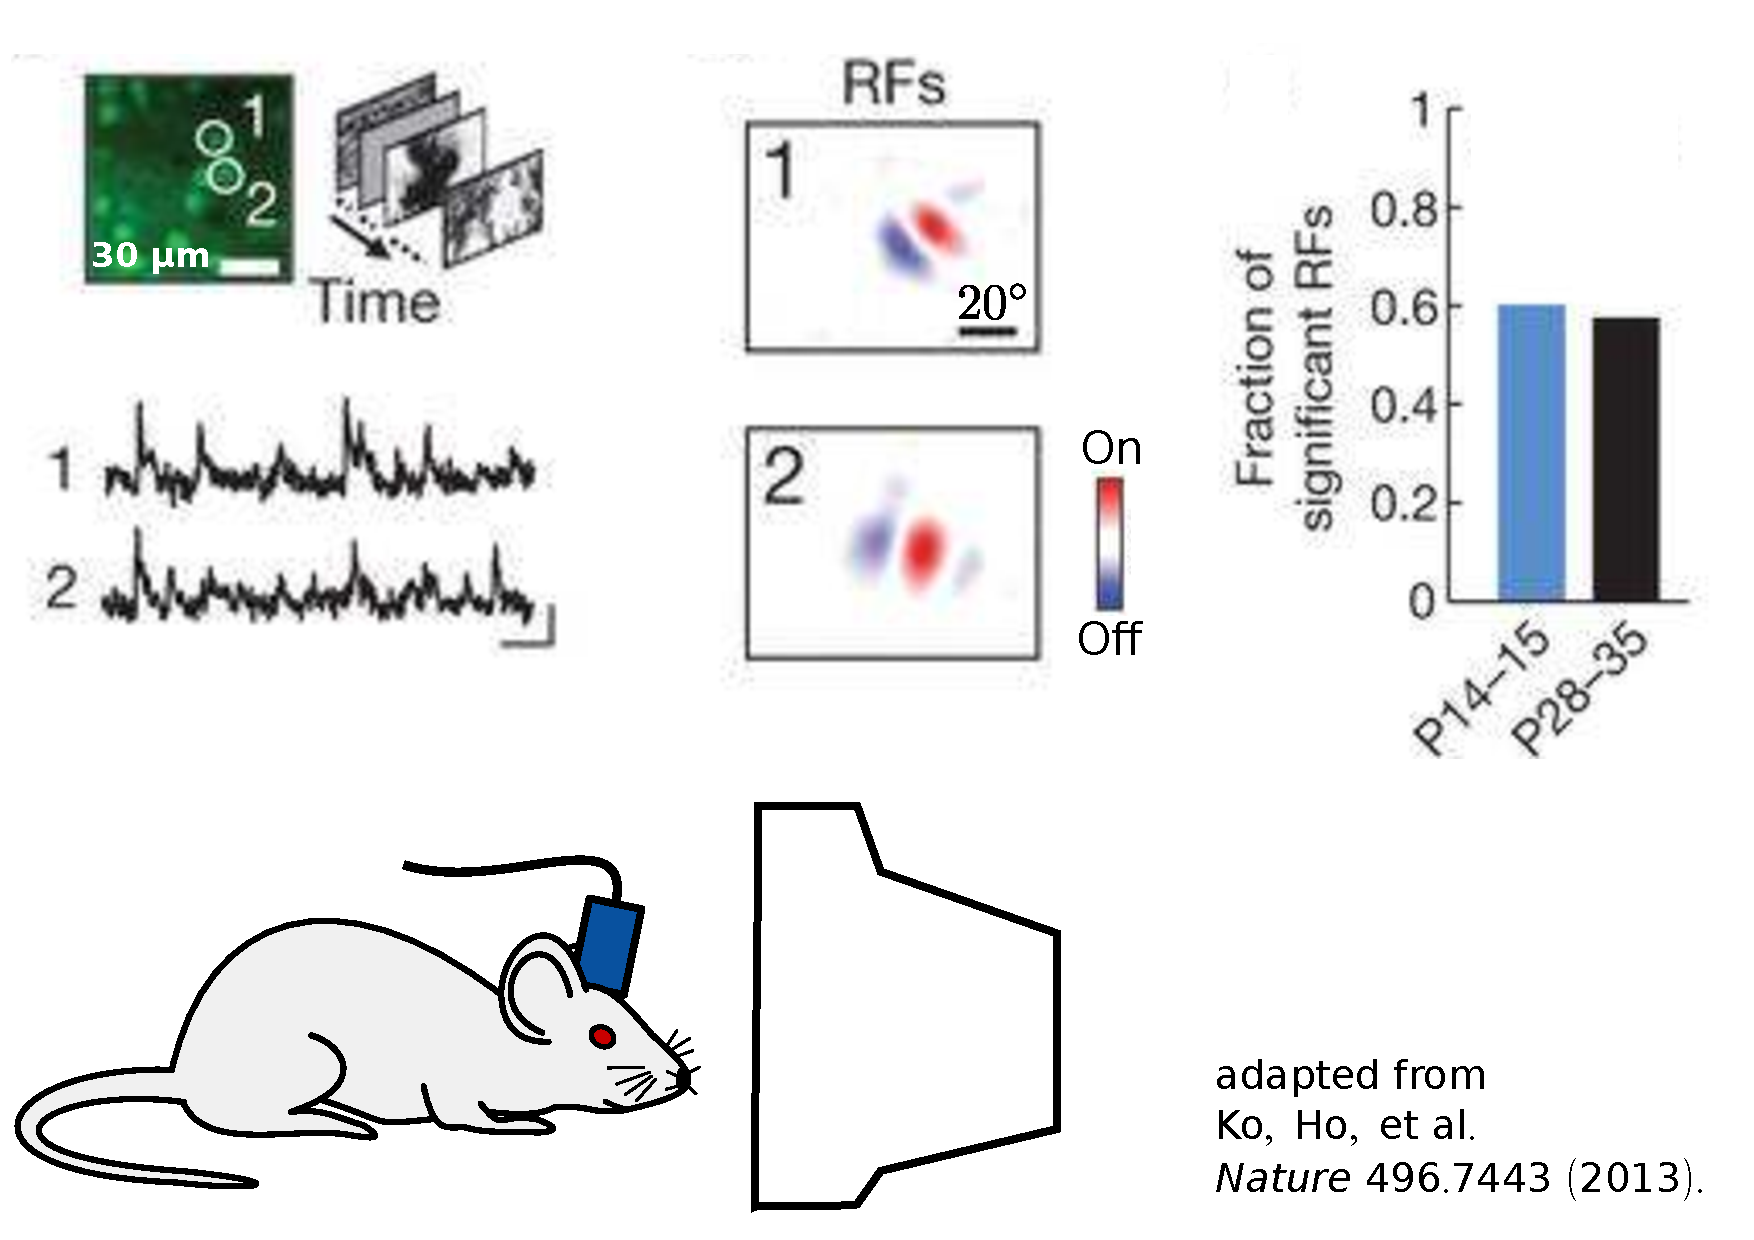
\includegraphics[height=0.9\textheight]{ko_rfs}
    }
\end{frame}

\begin{frame}[t]{Experimental results}
    \only<1>{
    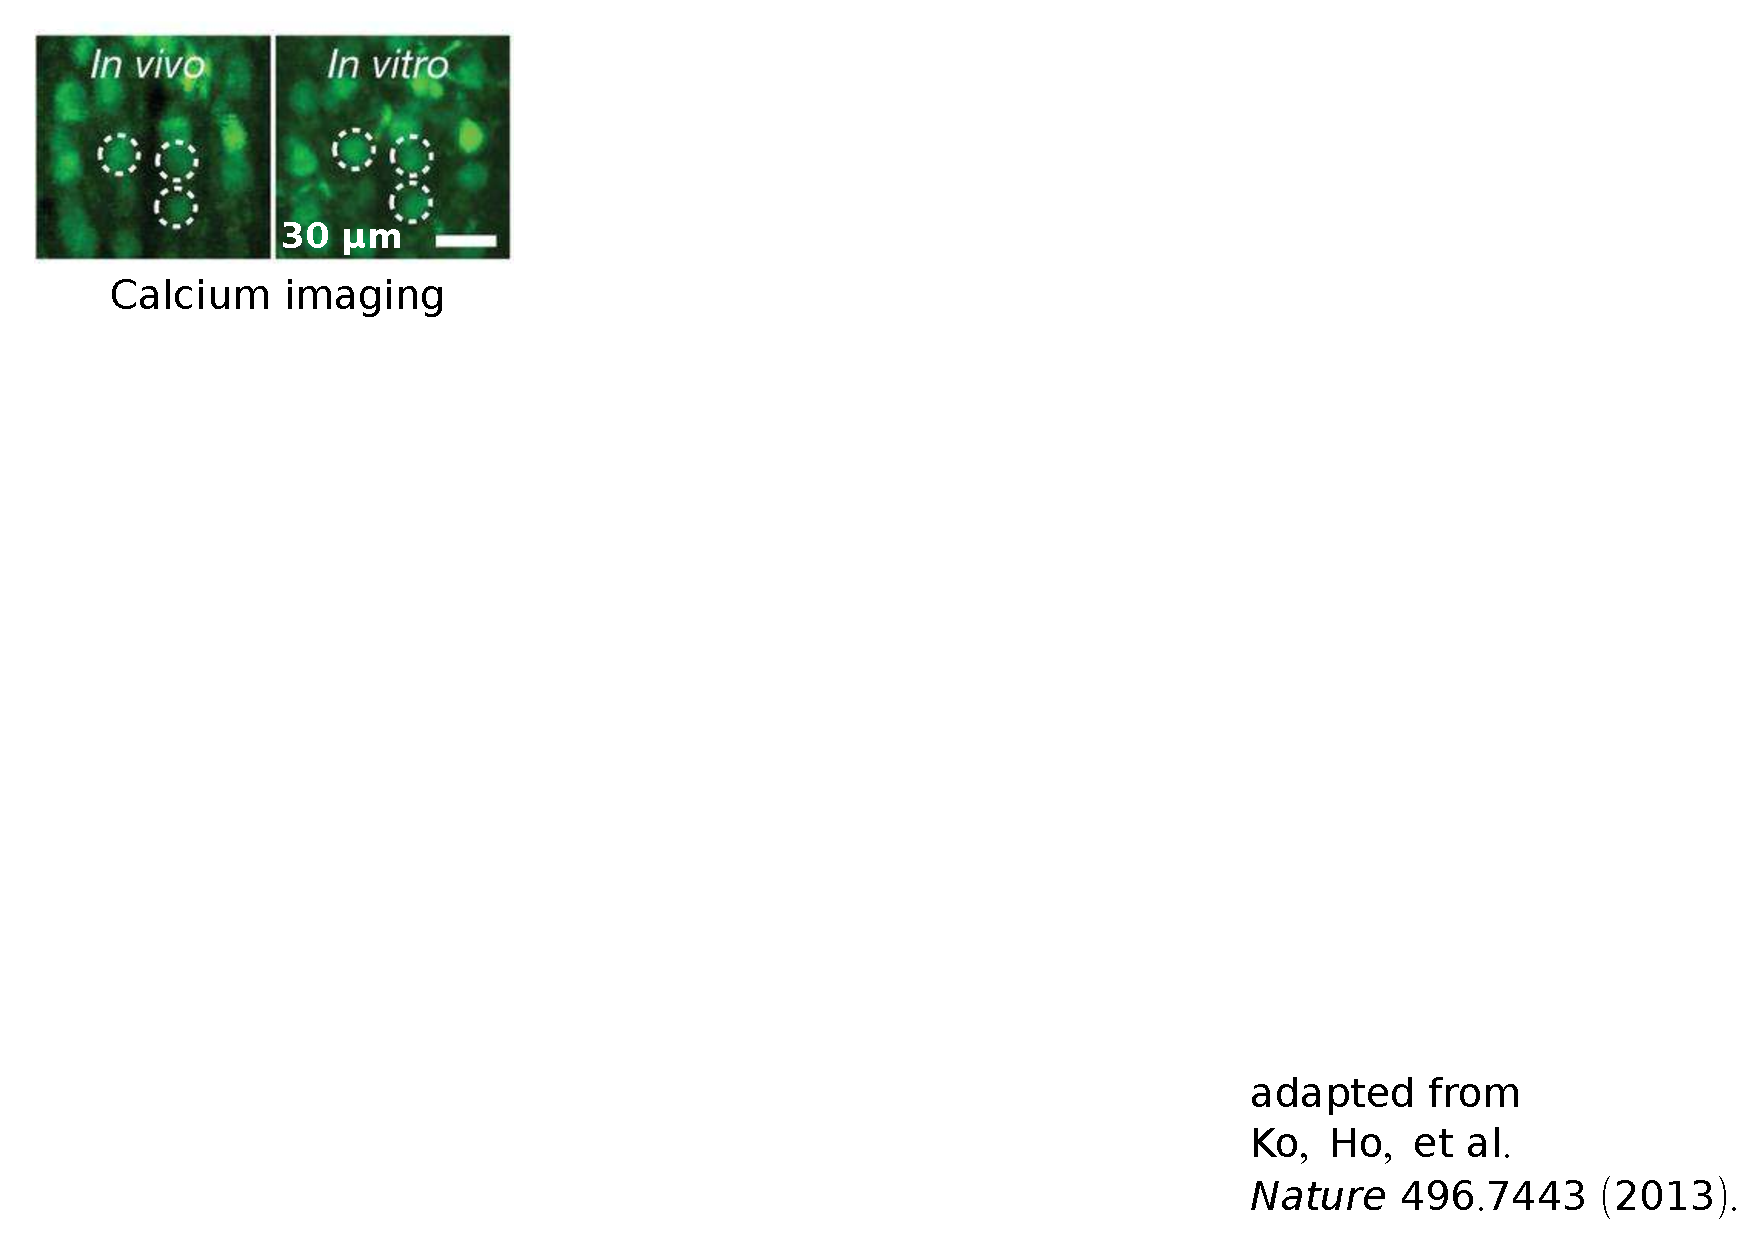
\includegraphics[height=0.9\textheight]{ko_results1}
    }
    \only<2>{
    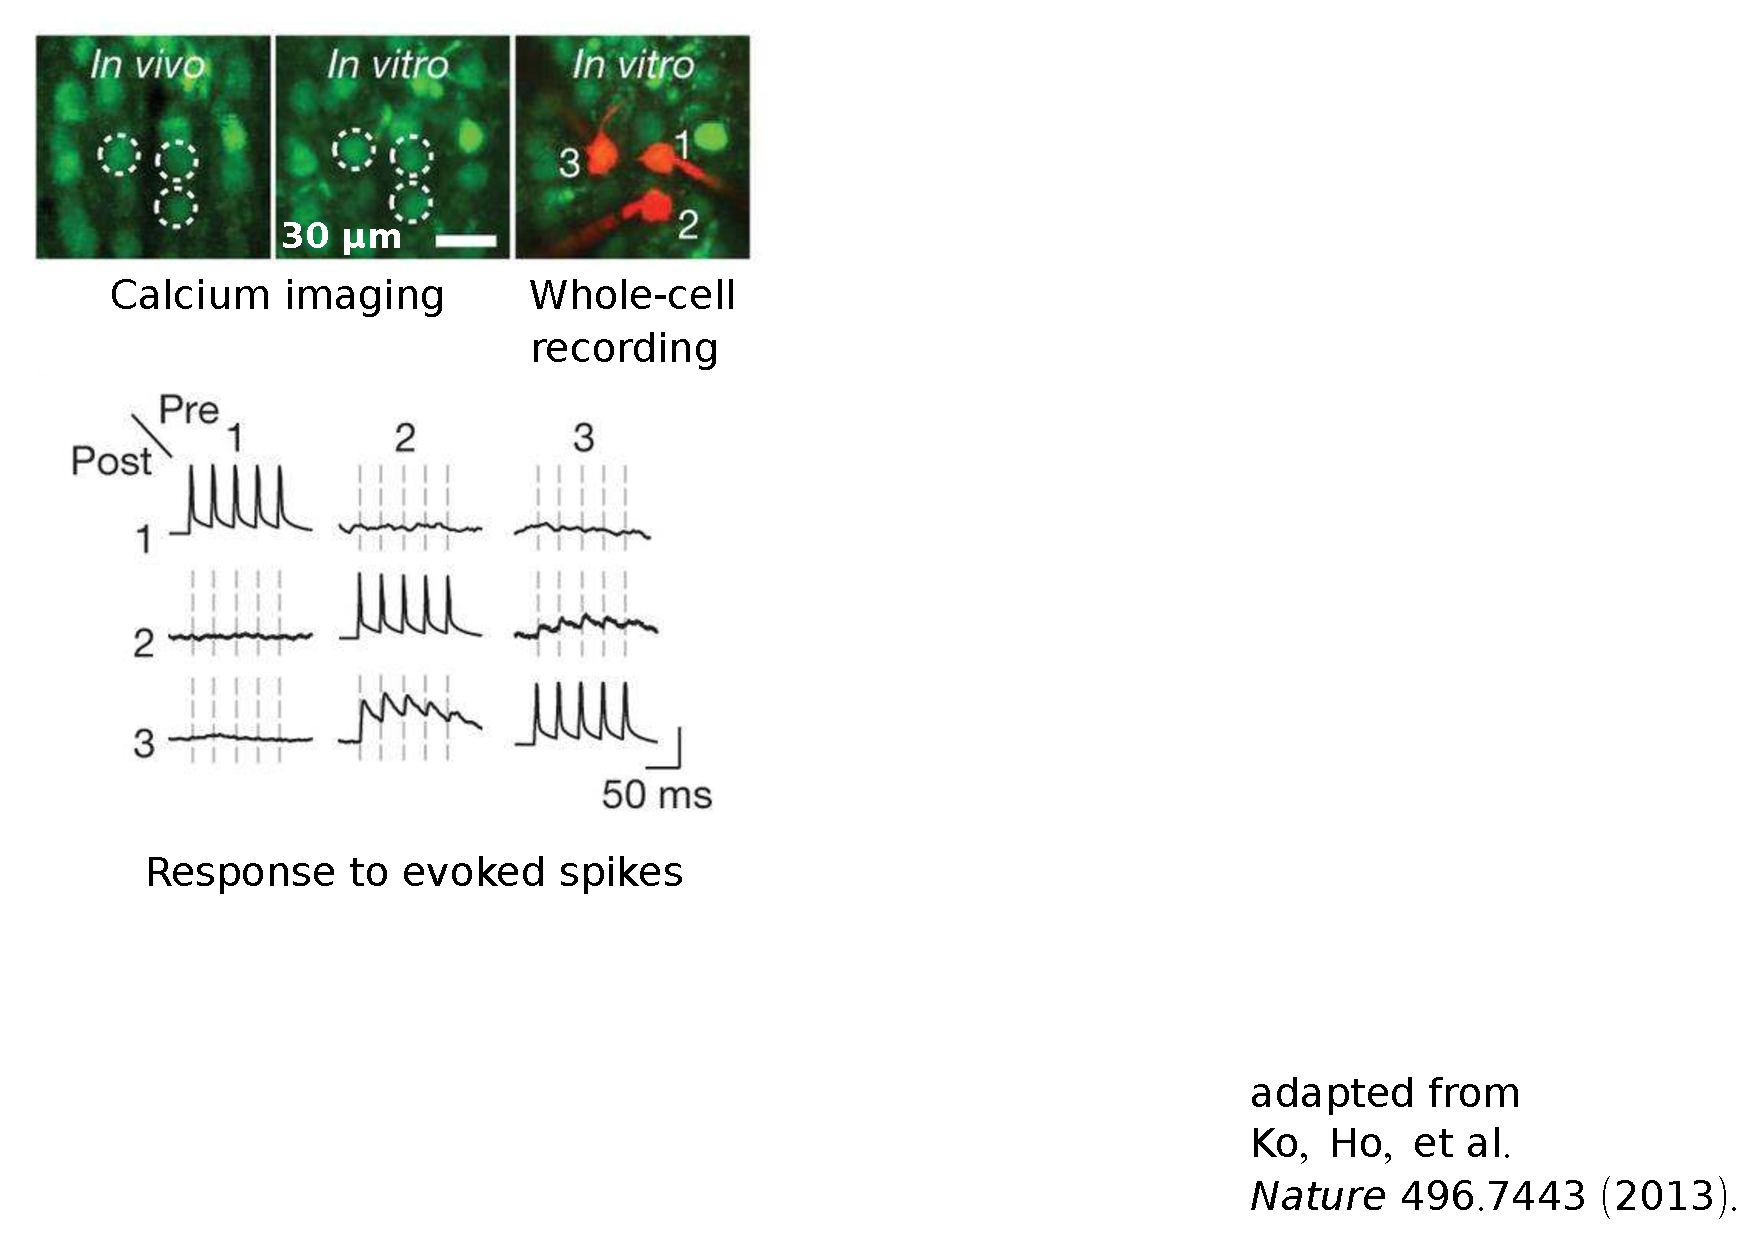
\includegraphics[height=0.9\textheight]{ko_results2}
    }
    \only<3>{
    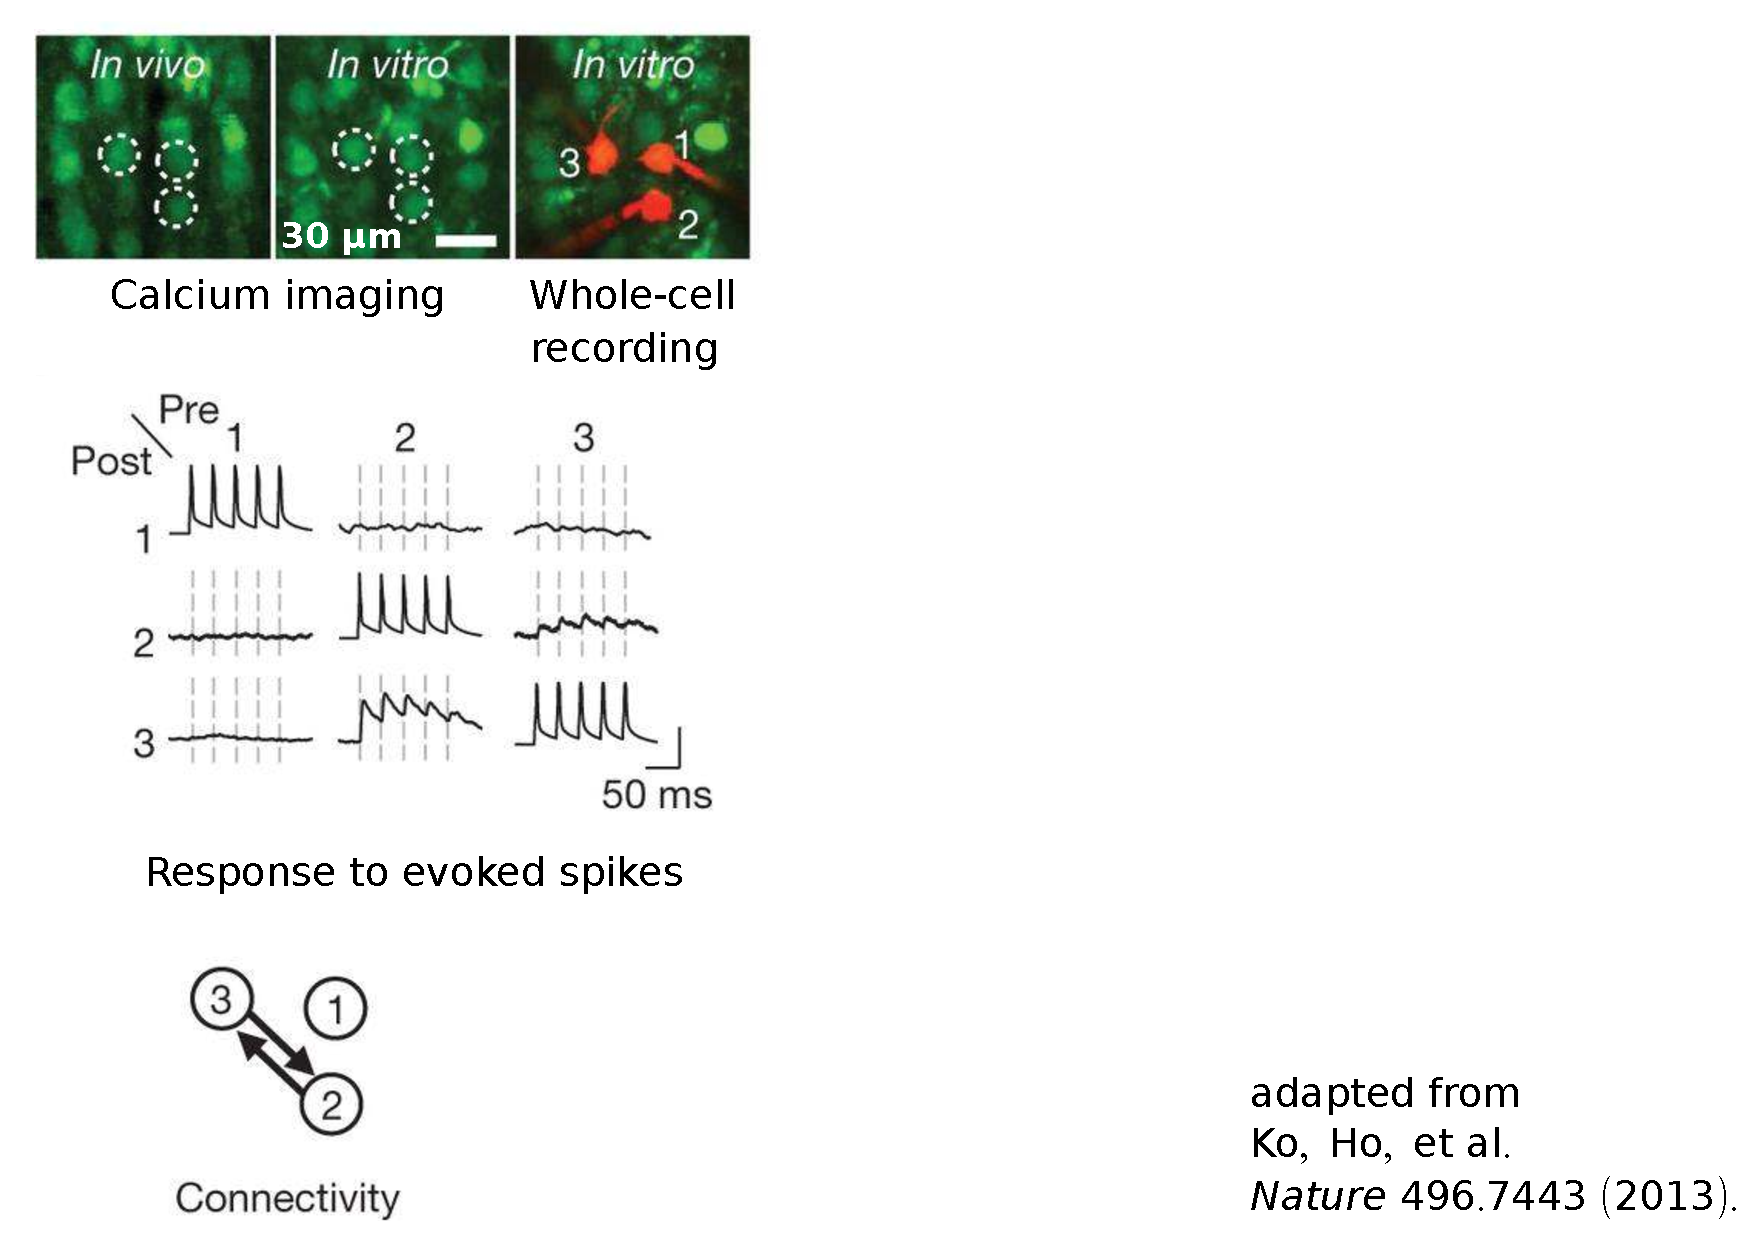
\includegraphics[height=0.9\textheight]{ko_results3}
    }
    \only<4>{
    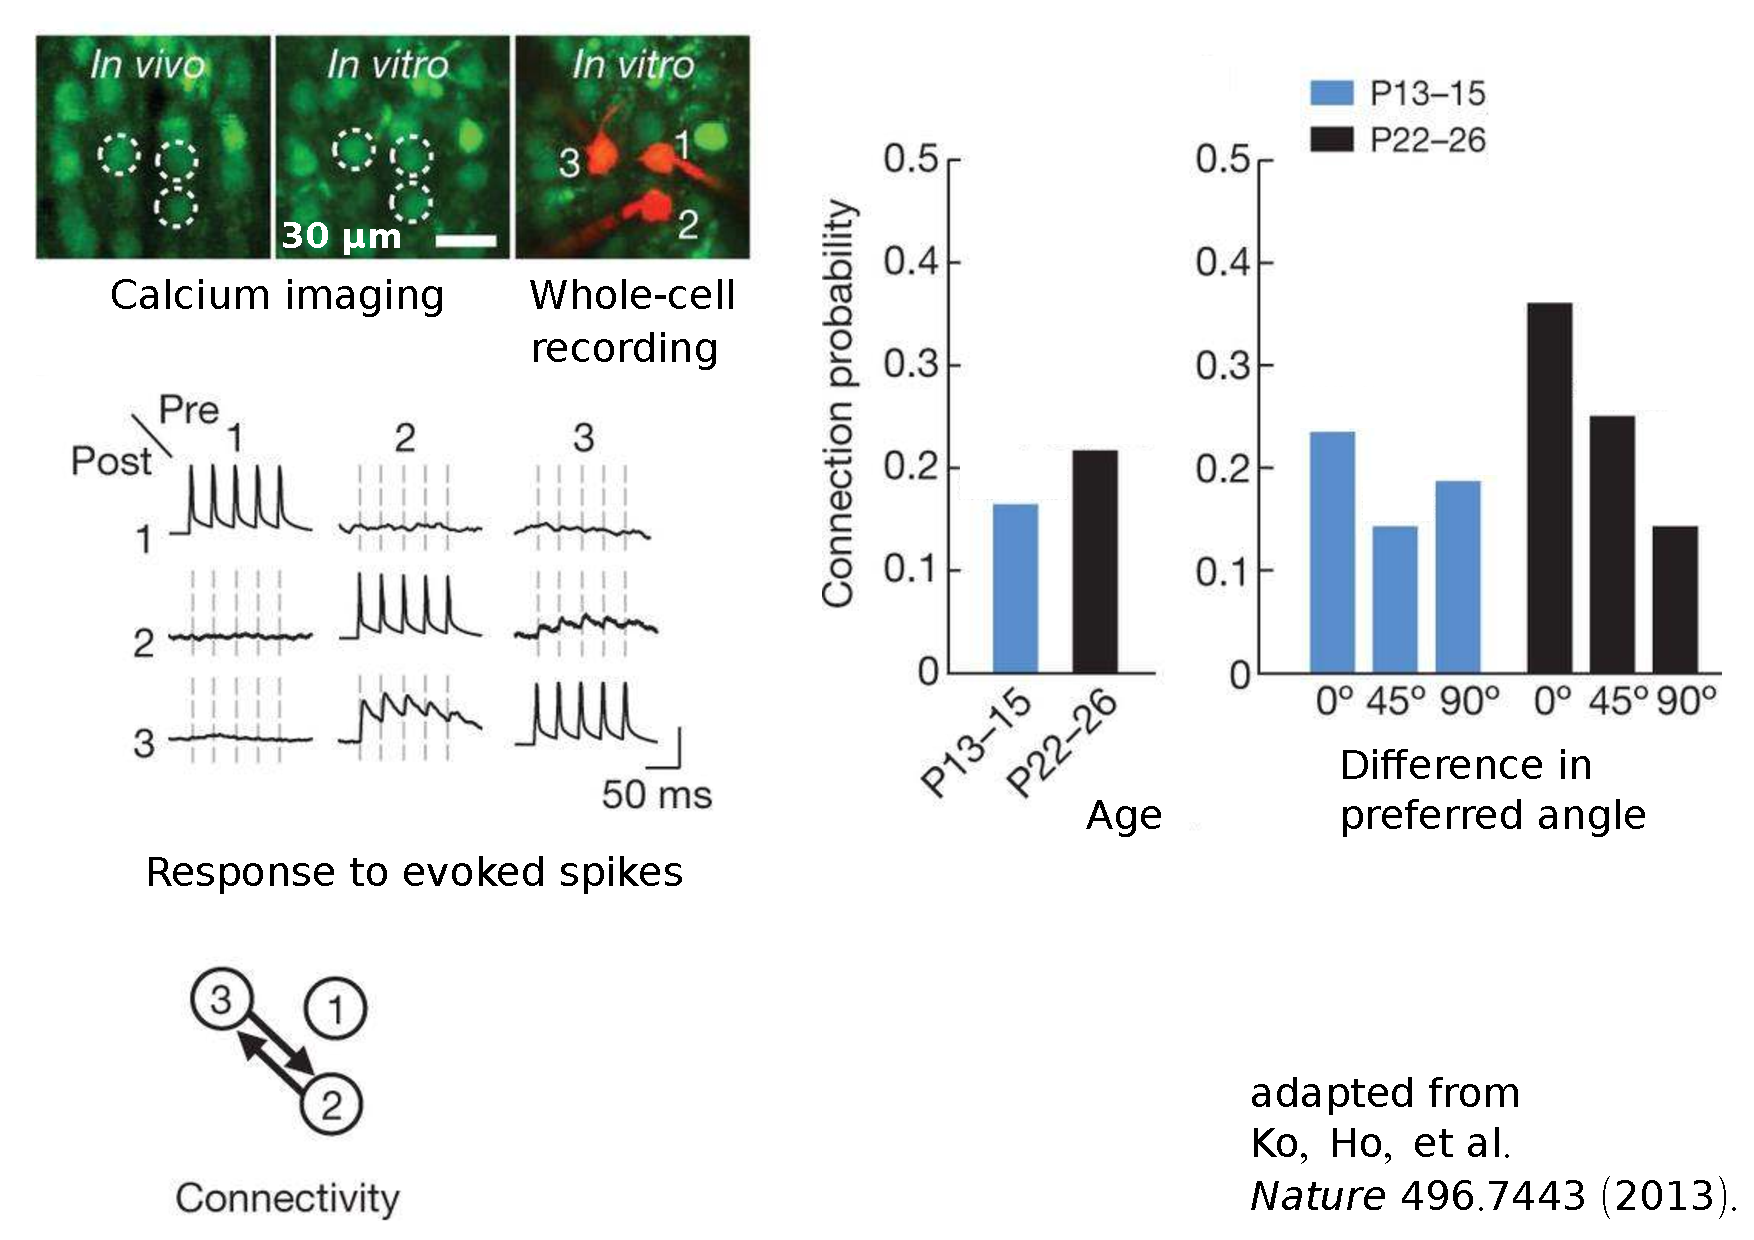
\includegraphics[height=0.9\textheight]{ko_results}
    }
\end{frame}

% Experiment -- Theory?
\begin{frame}[t]{}
    \vspace{3.5cm}
    \huge Experiment \qquad $\implies$ \qquad Theory
\end{frame}

% Sadra's Model
\begin{frame}[t]{Functional specificity in a model}
    \only<1>{
    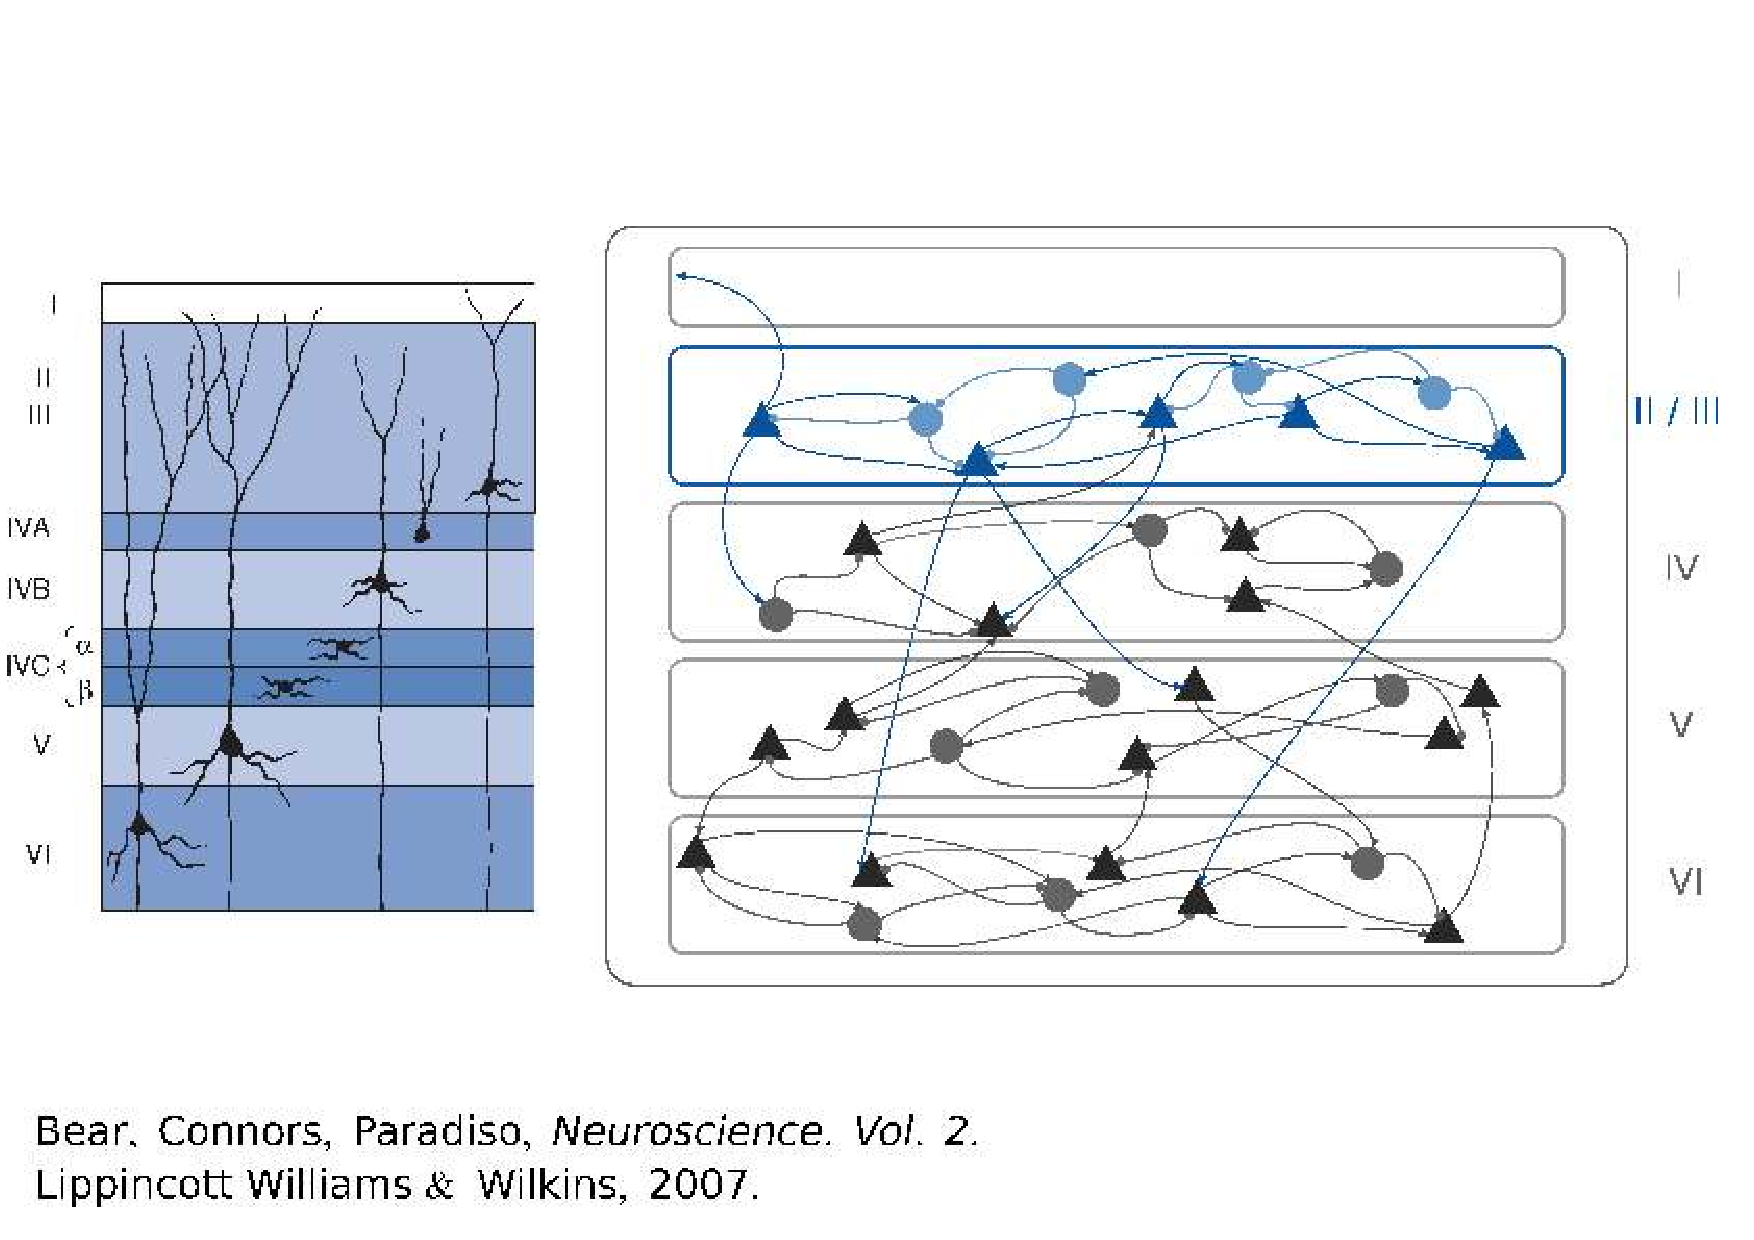
\includegraphics[height=0.9\textheight]{layers}
    }
    \only<2>{
    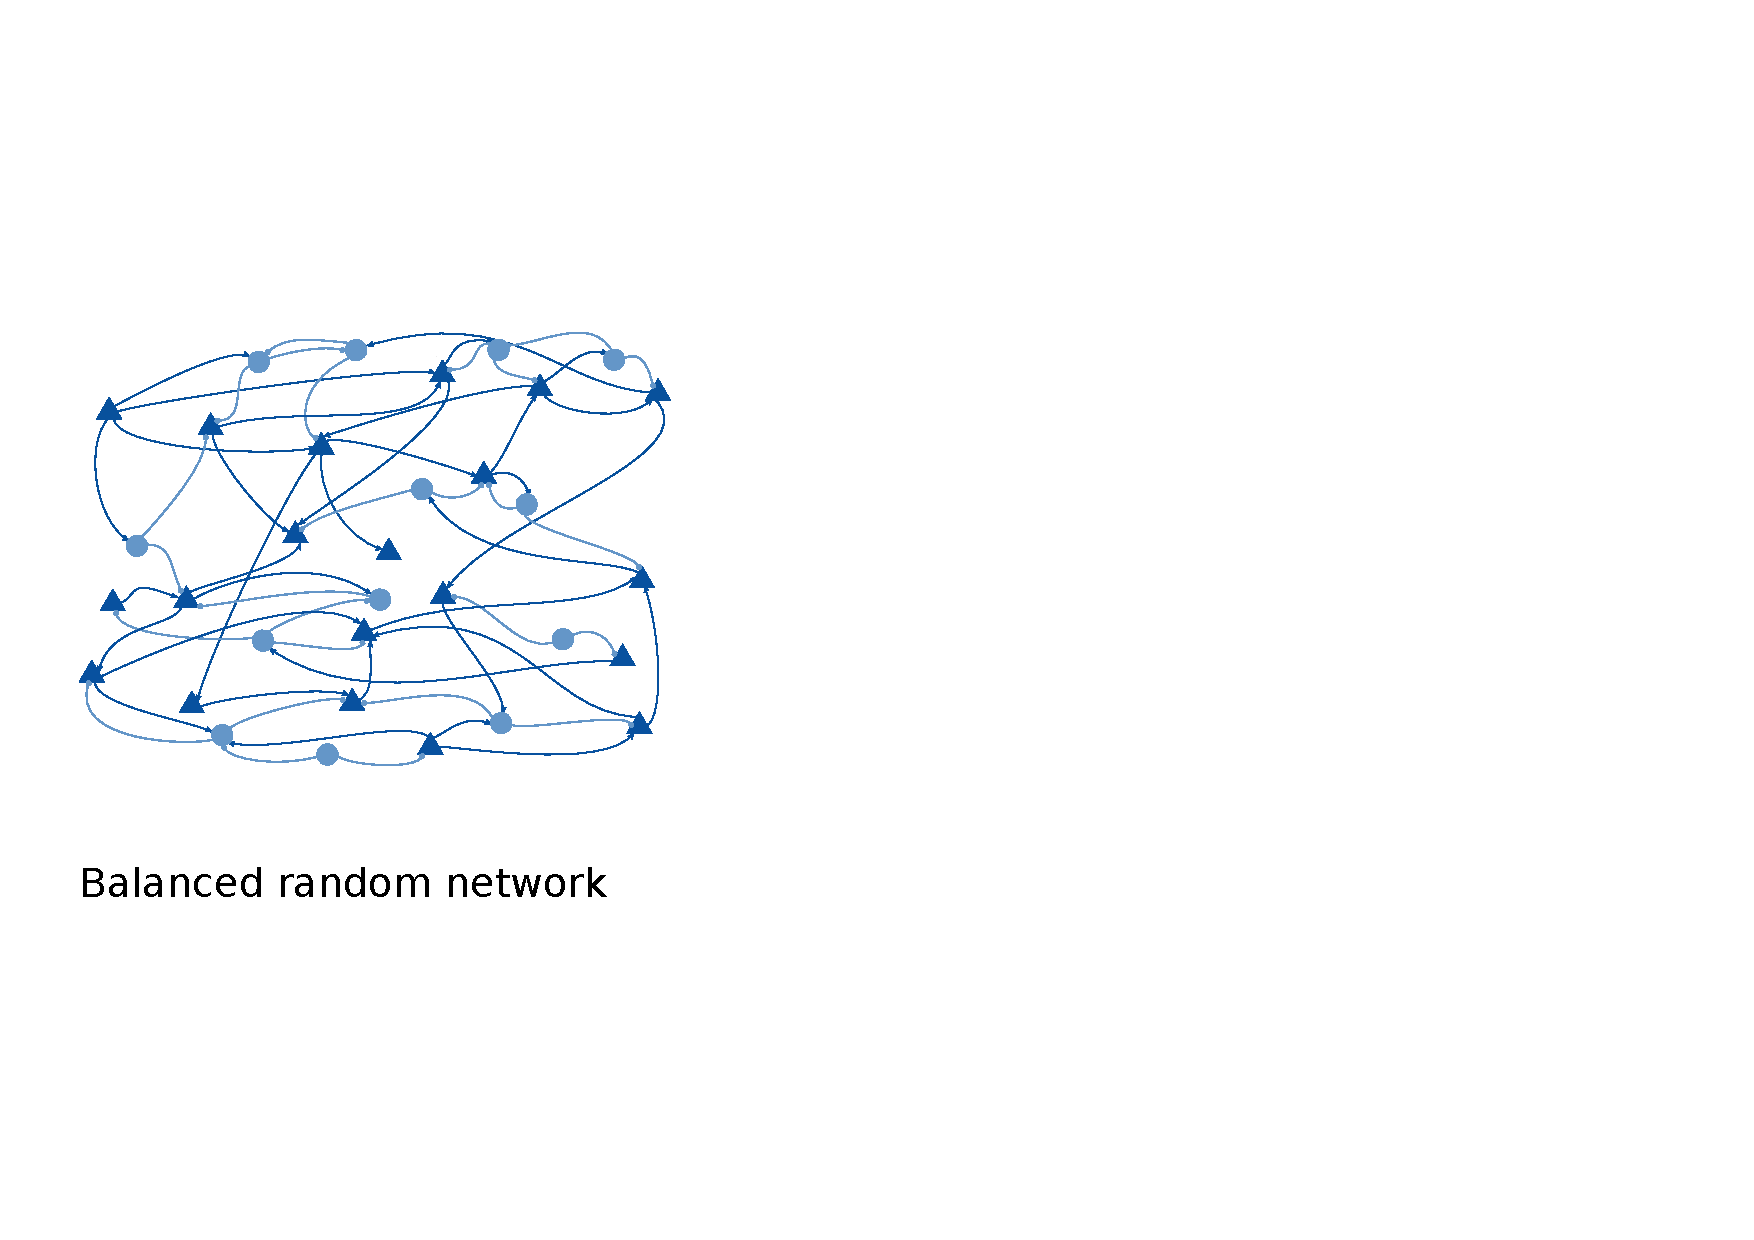
\includegraphics[height=0.9\textheight]{random_and_stdp1}
    }
    \only<3>{
    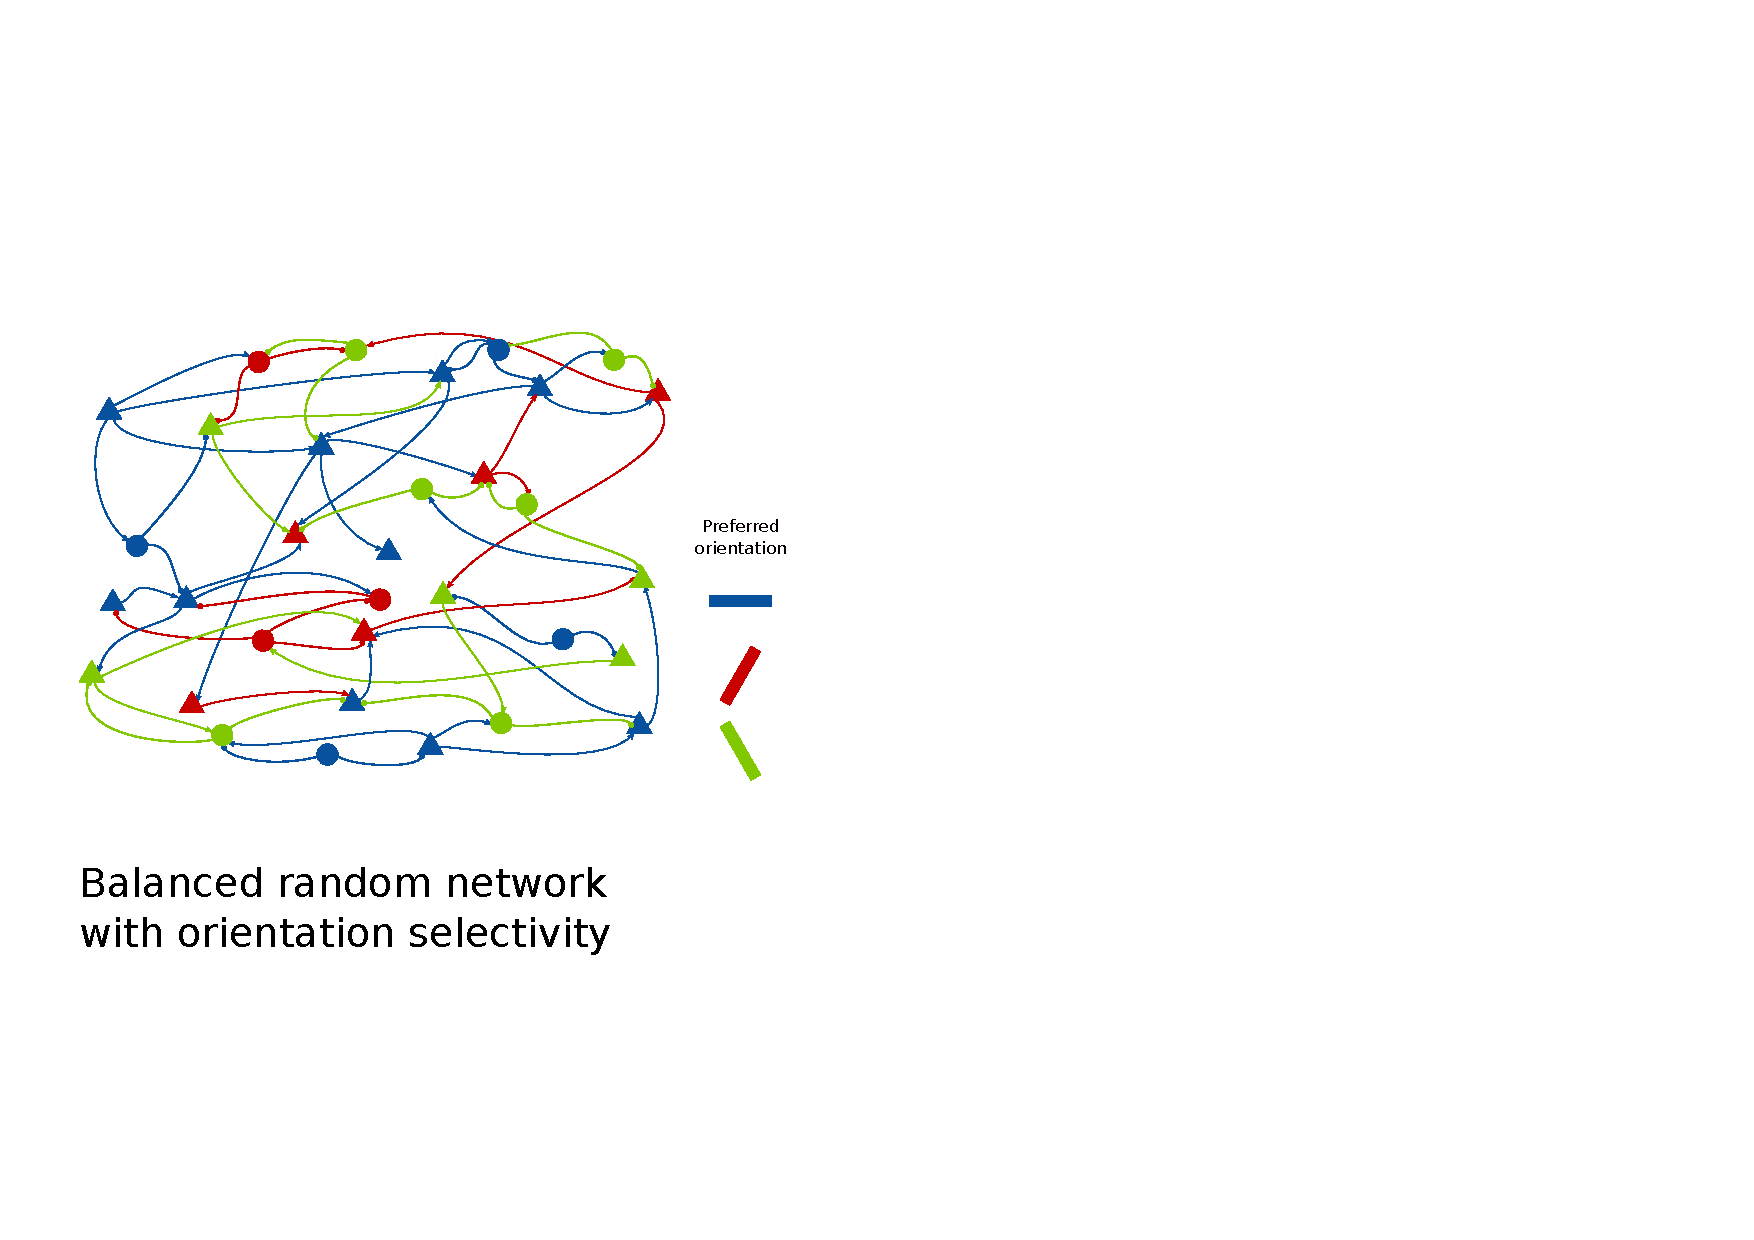
\includegraphics[height=0.9\textheight]{random_and_stdp2}
    }
    \only<4>{
    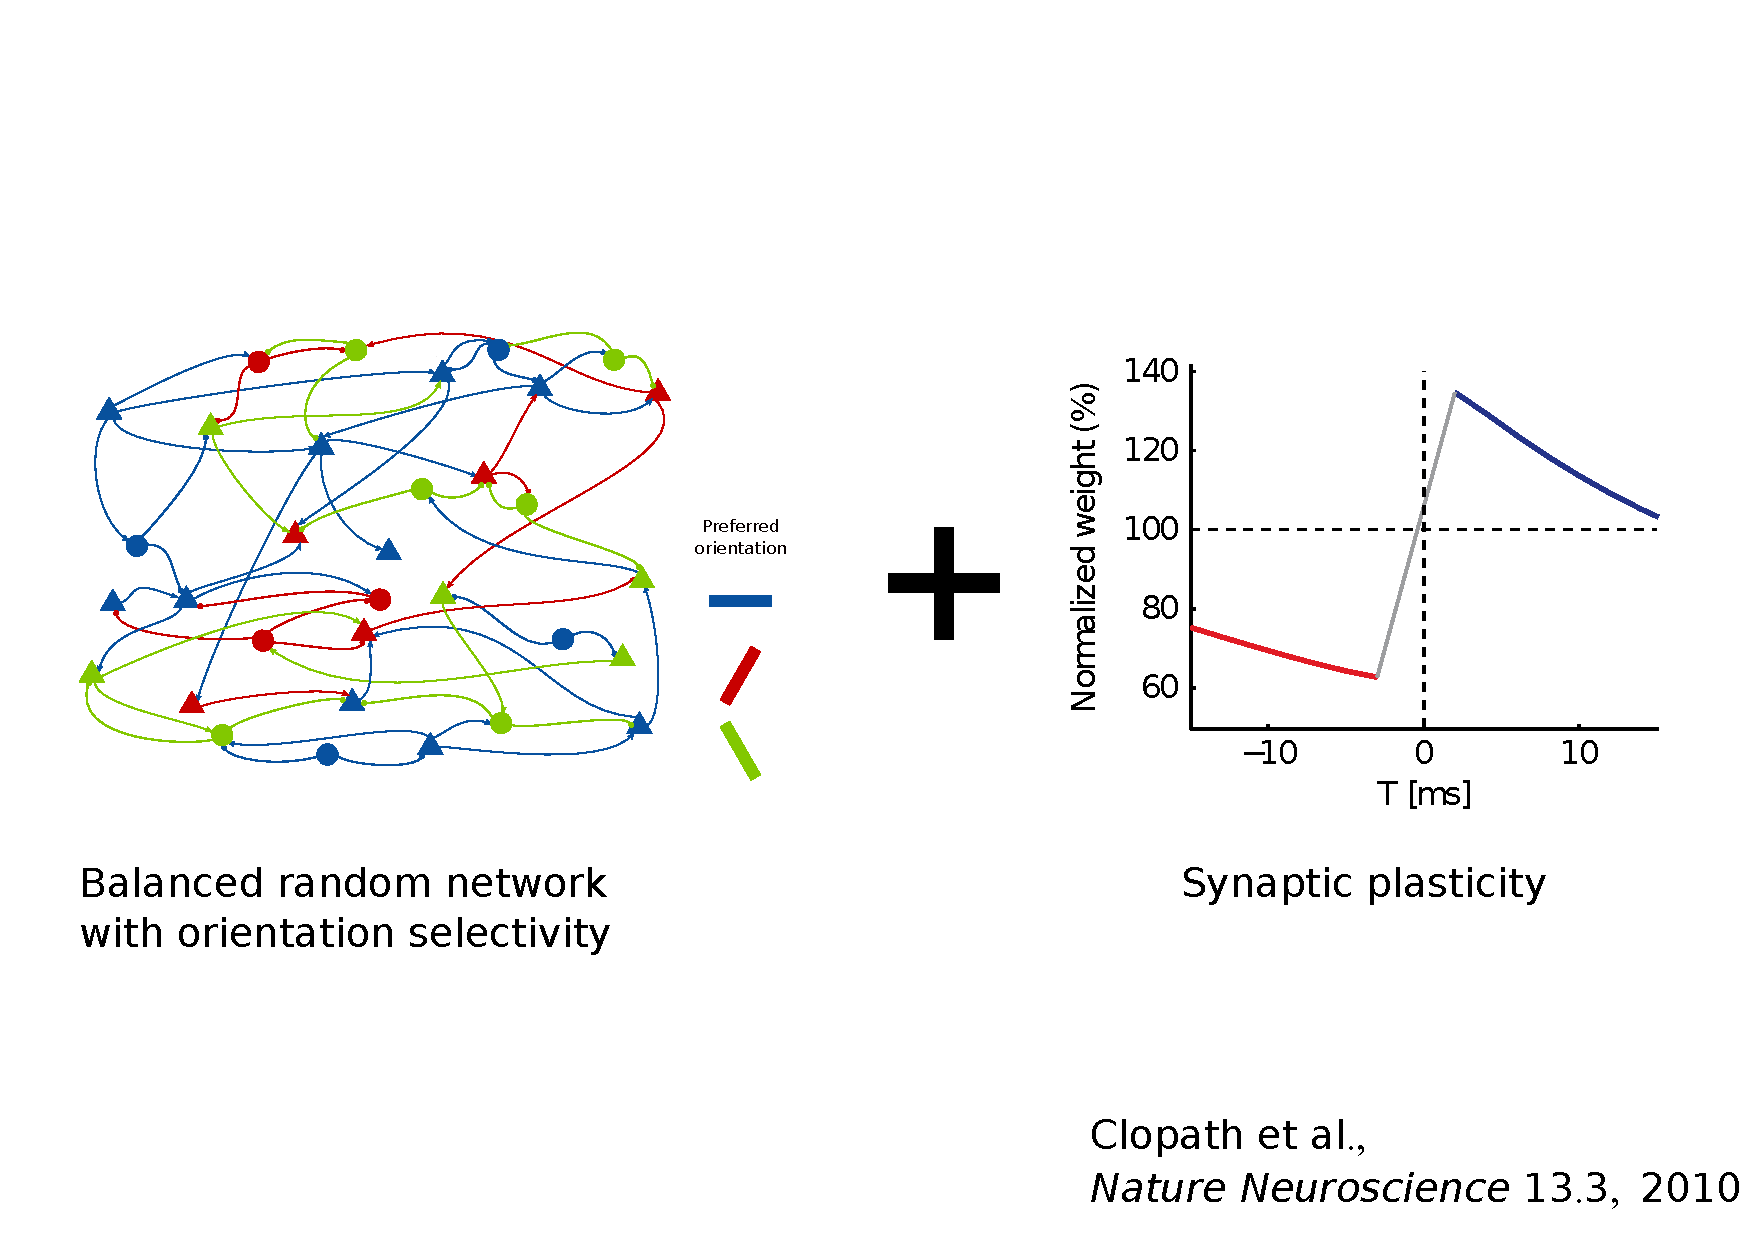
\includegraphics[height=0.9\textheight]{random_and_stdp3}
    }
    \only<5>{
    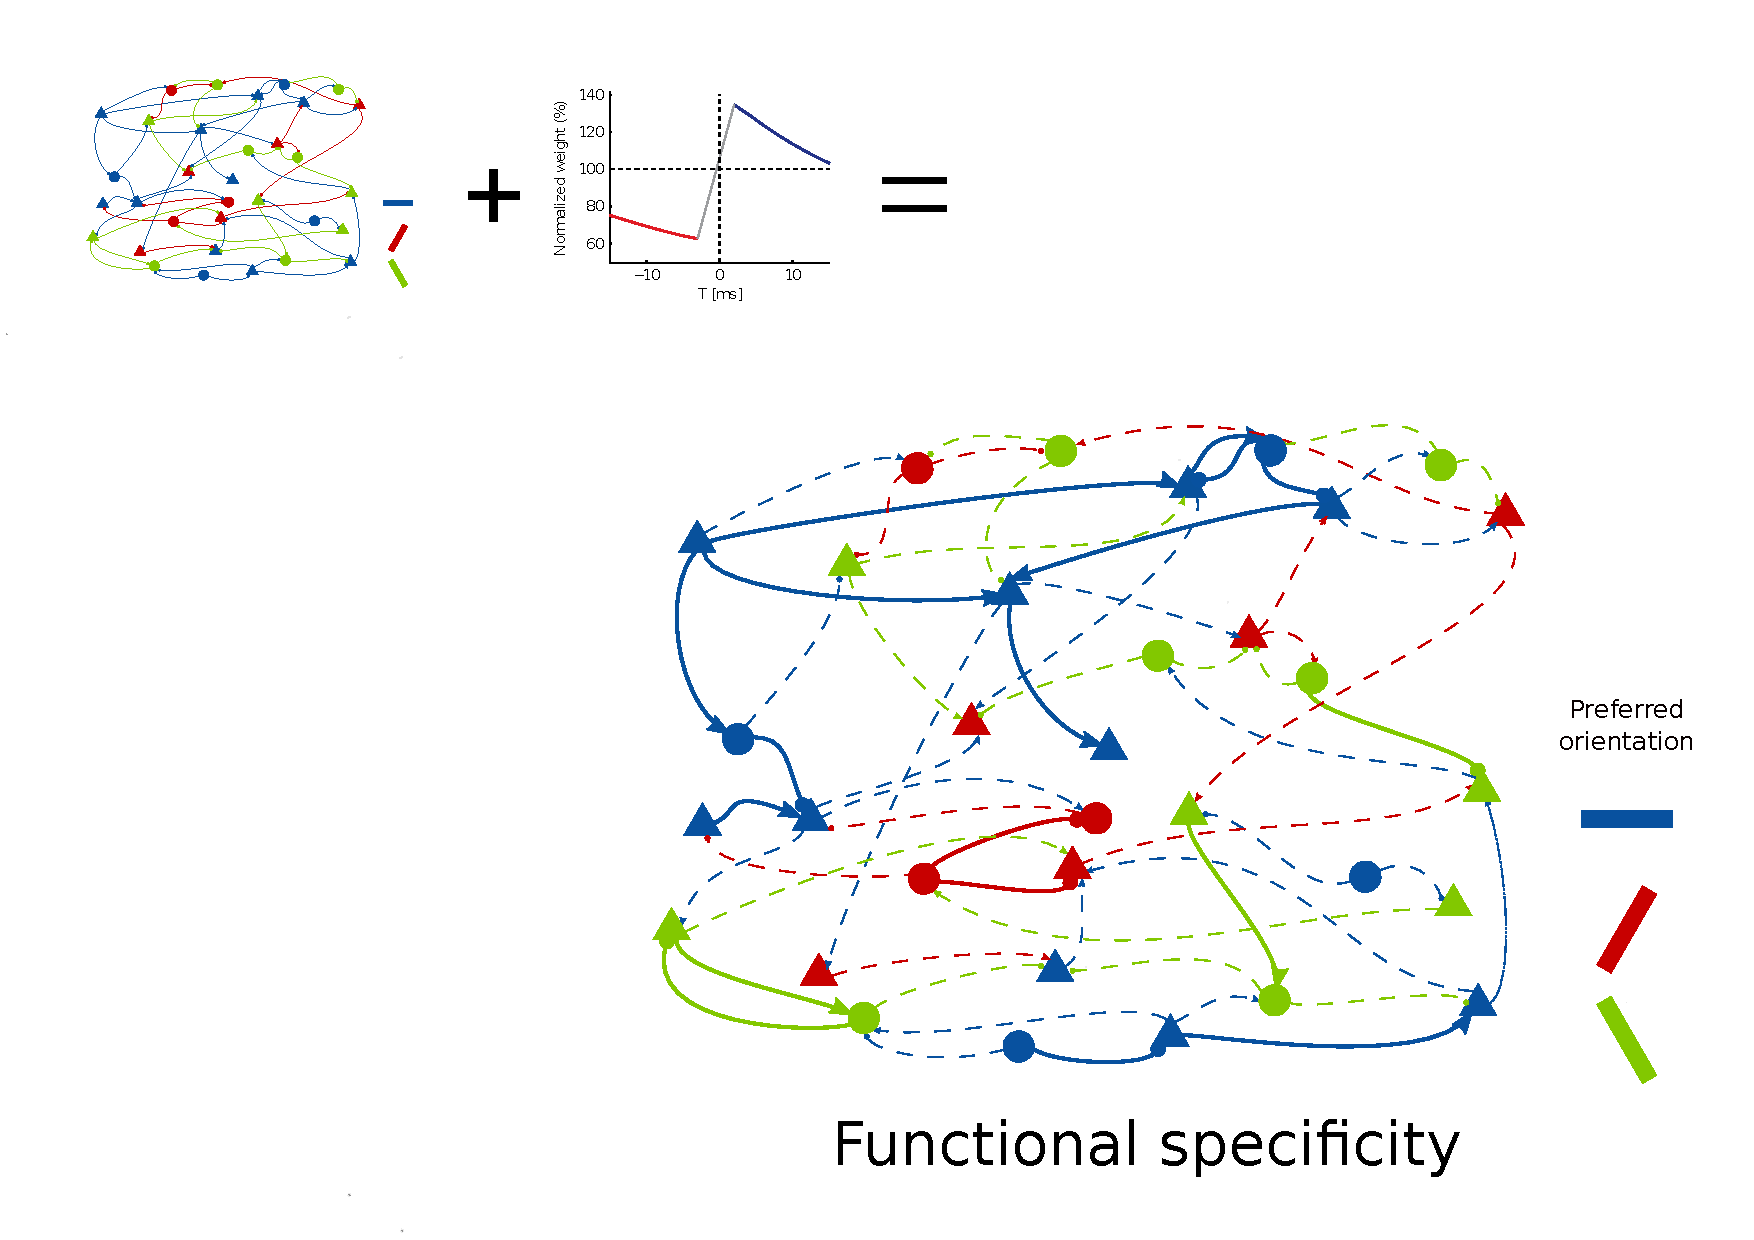
\includegraphics[height=0.9\textheight]{random_and_stdp}
    }
\end{frame}

% Sadra's results
\begin{frame}[t]{Population activity}
    \only<1>{
    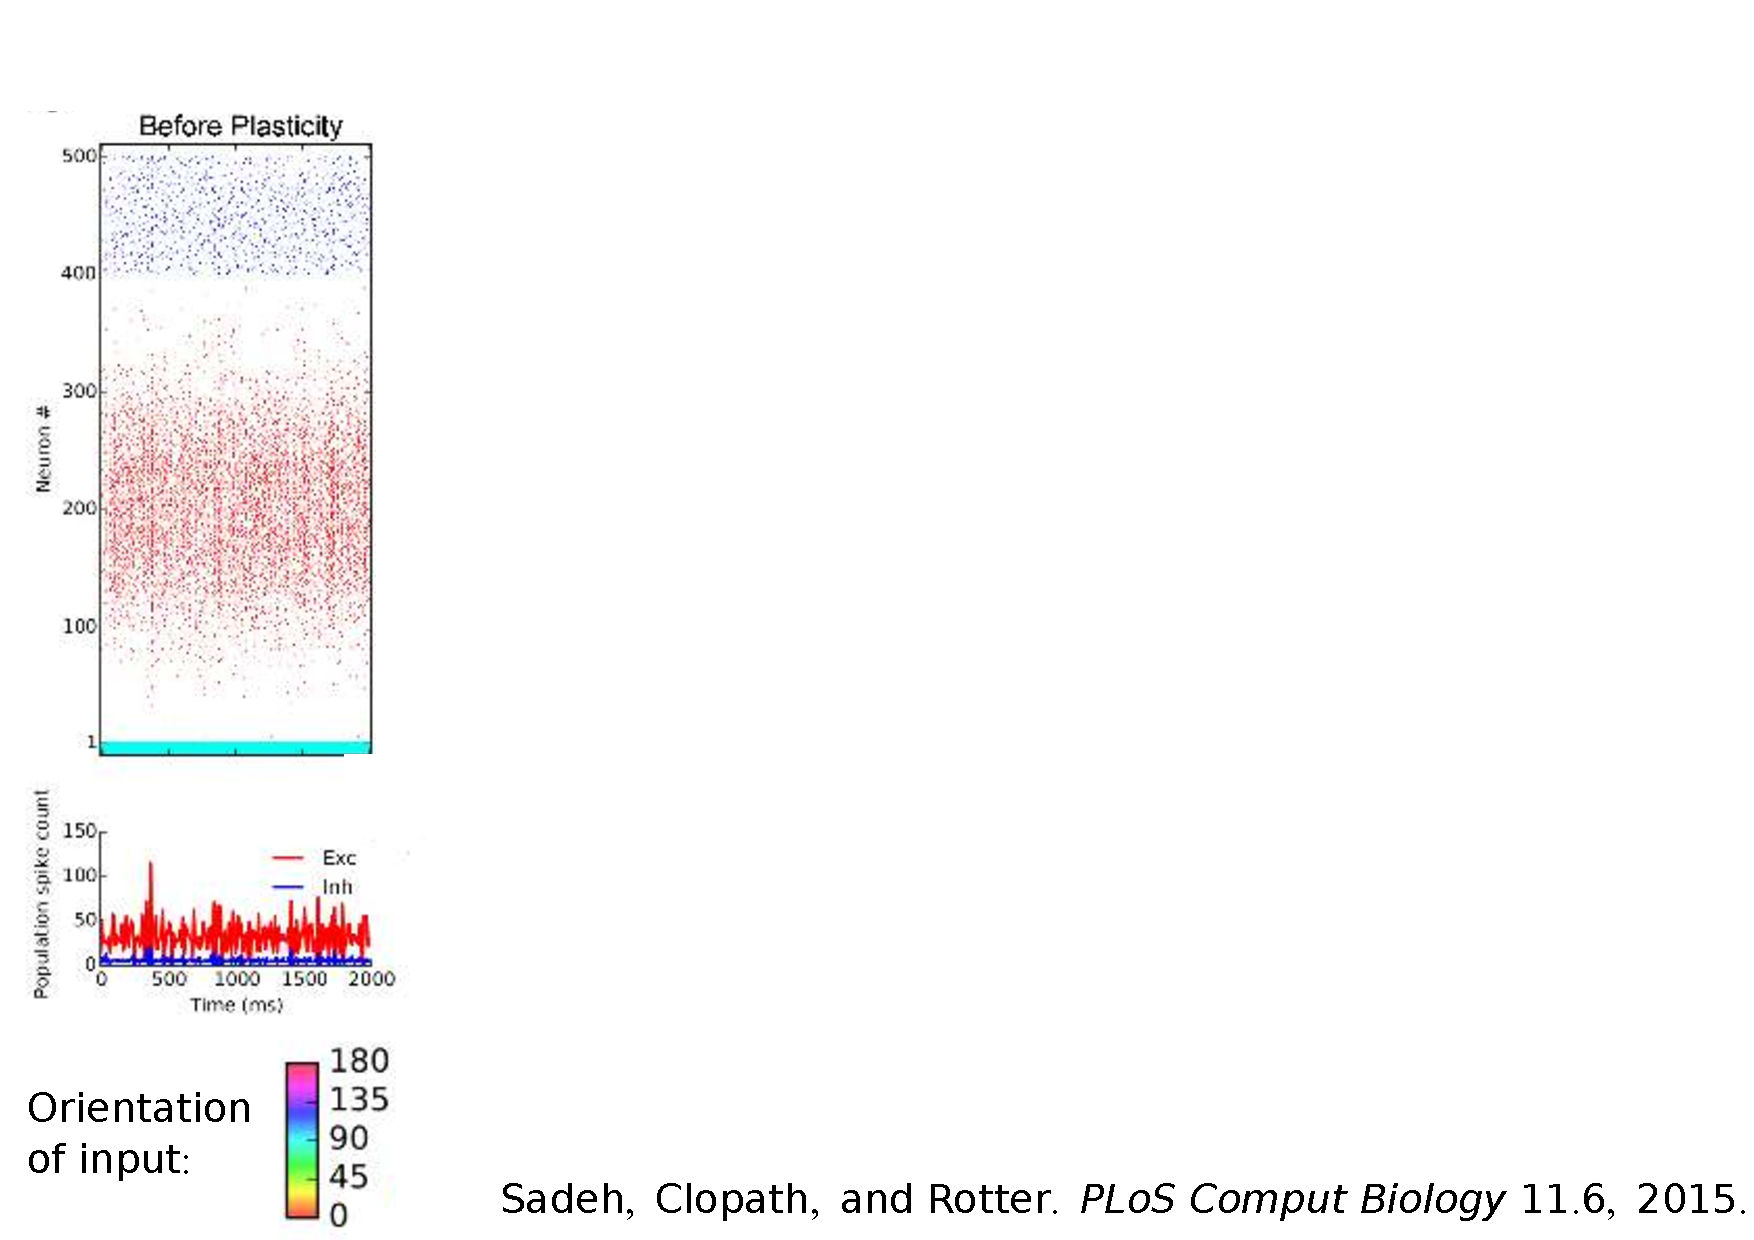
\includegraphics[height=0.9\textheight]{sadra_raster1}
    }
    \only<2>{
    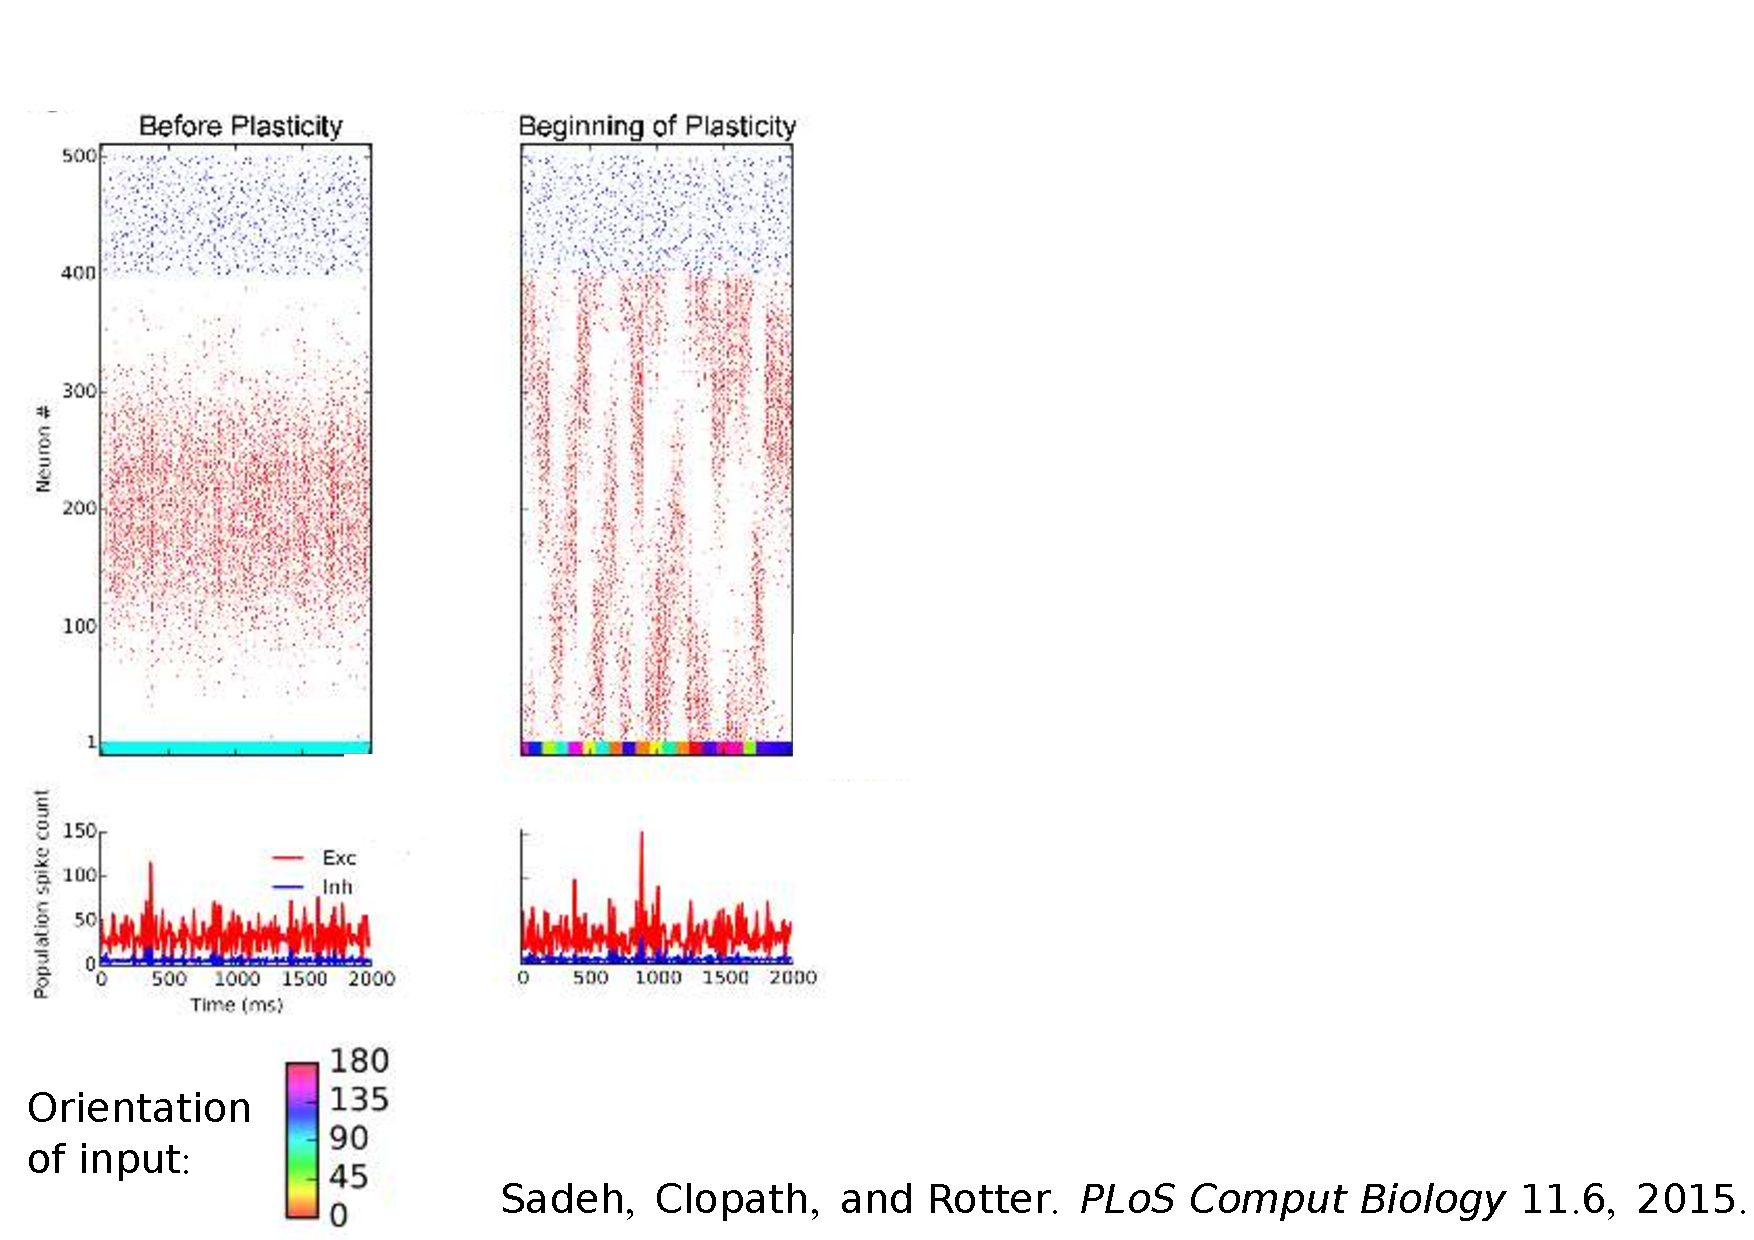
\includegraphics[height=0.9\textheight]{sadra_raster2}
    }
    \only<3>{
    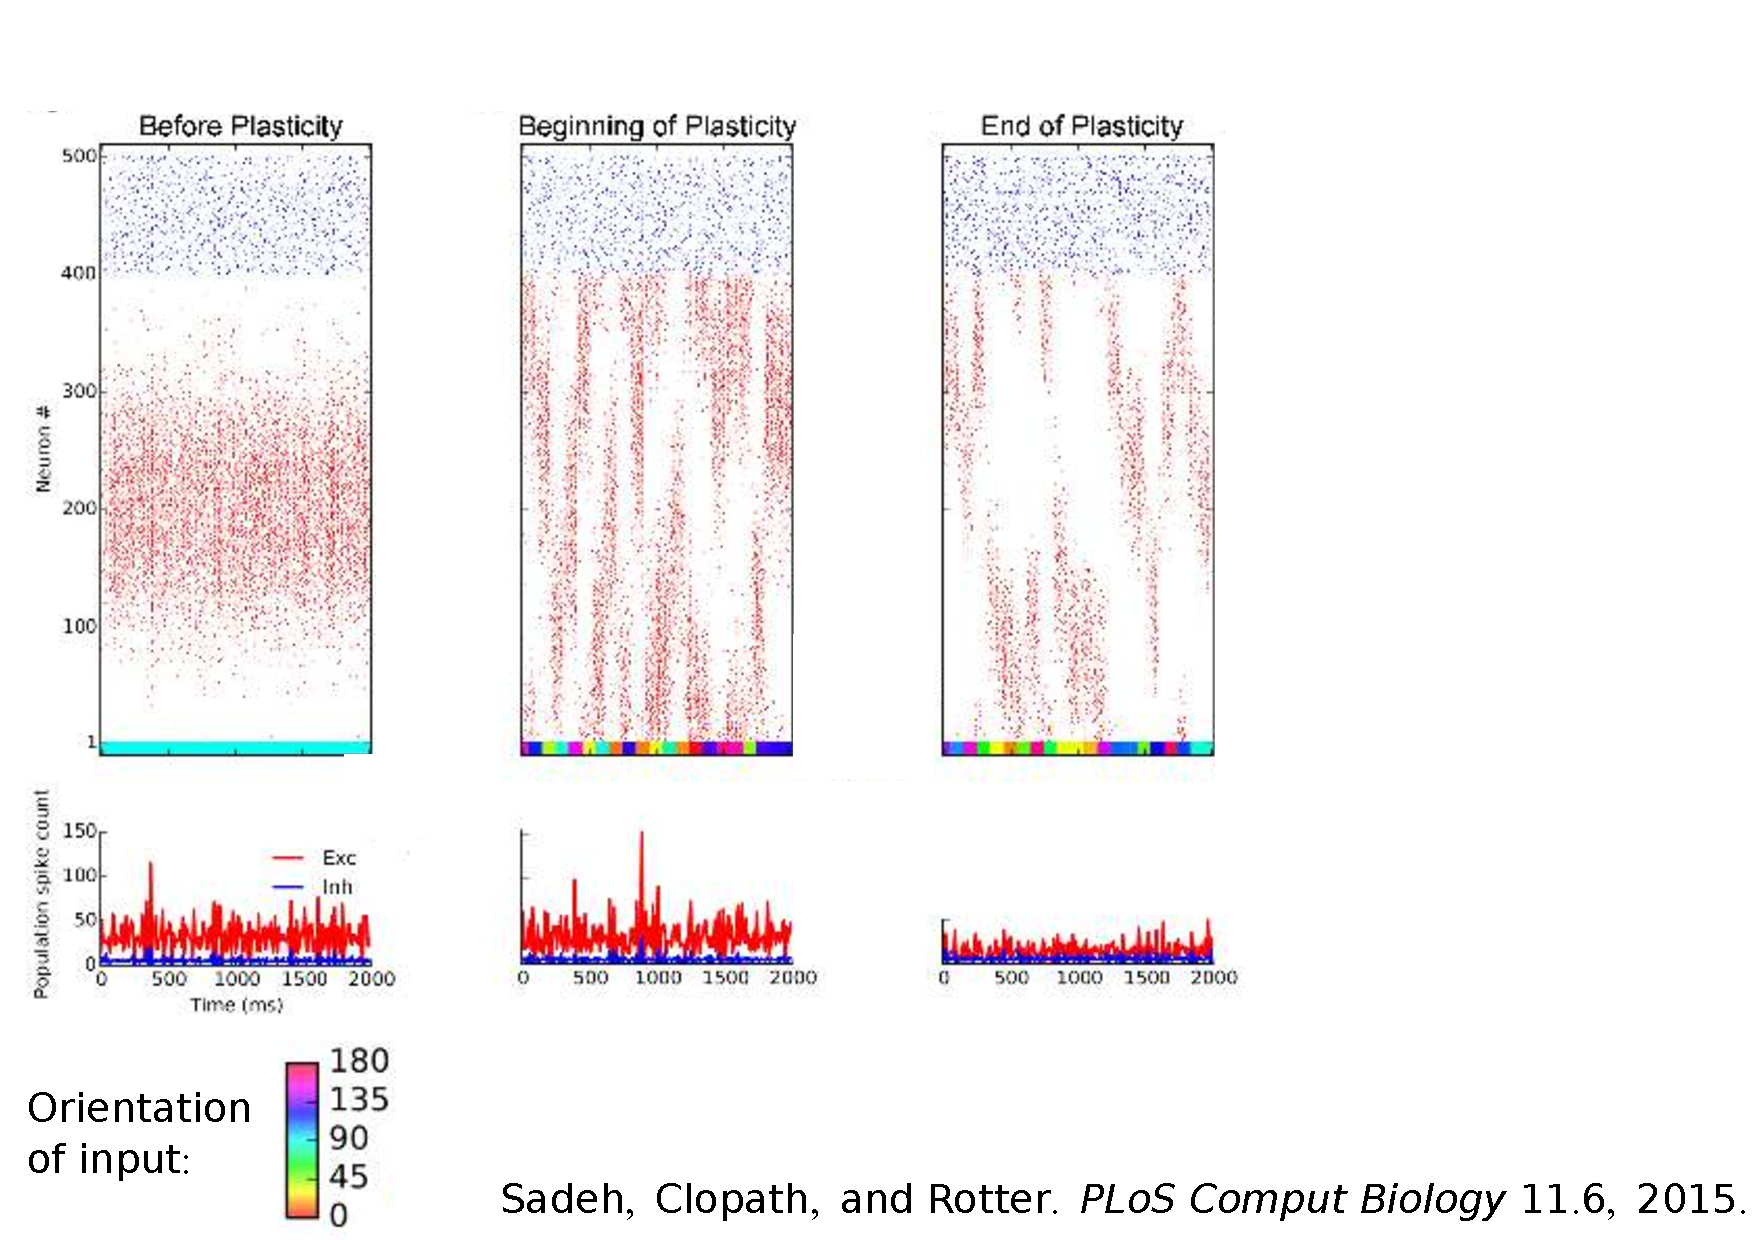
\includegraphics[height=0.9\textheight]{sadra_raster3}
    }
    \only<4>{
    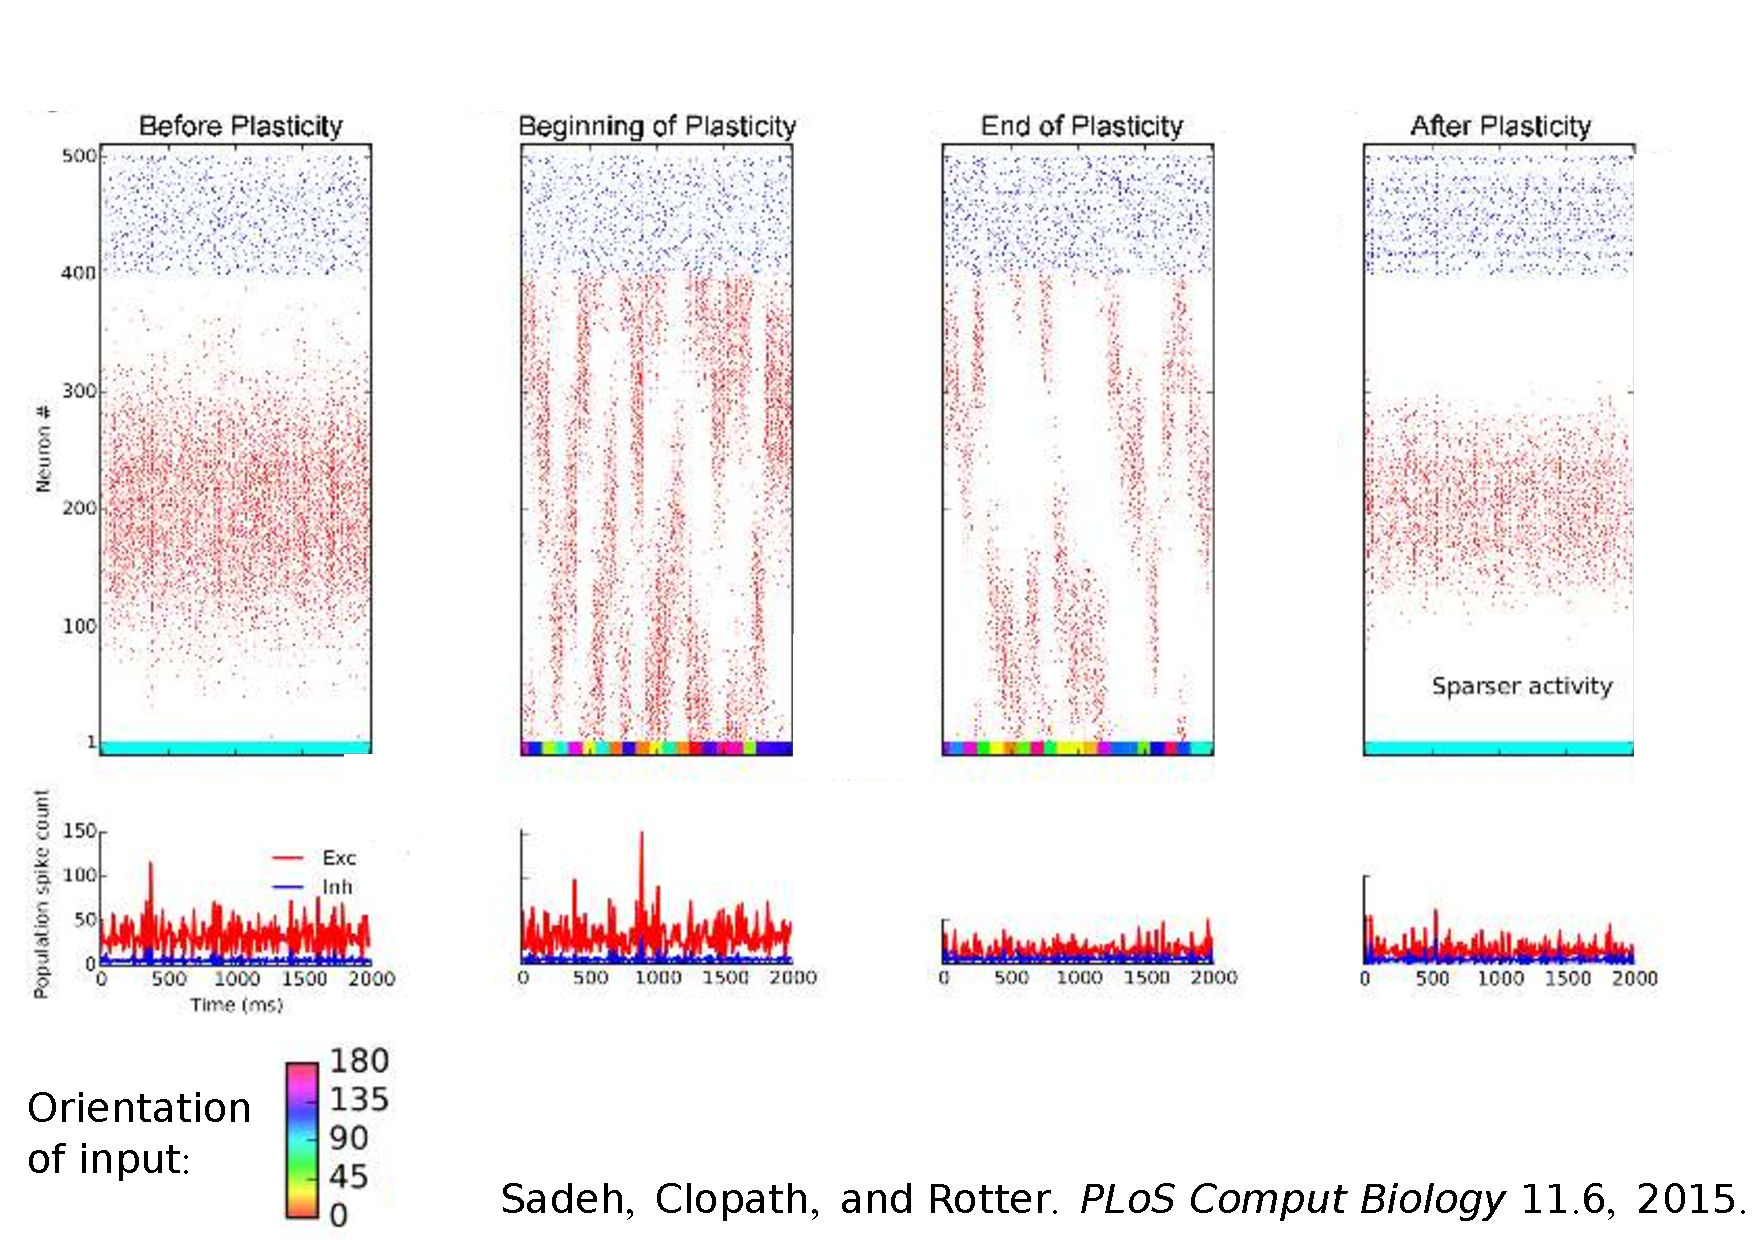
\includegraphics[height=0.9\textheight]{sadra_raster}
    }
\end{frame}

\begin{frame}[t]{Changing tuning curves}
    \only<1>{
    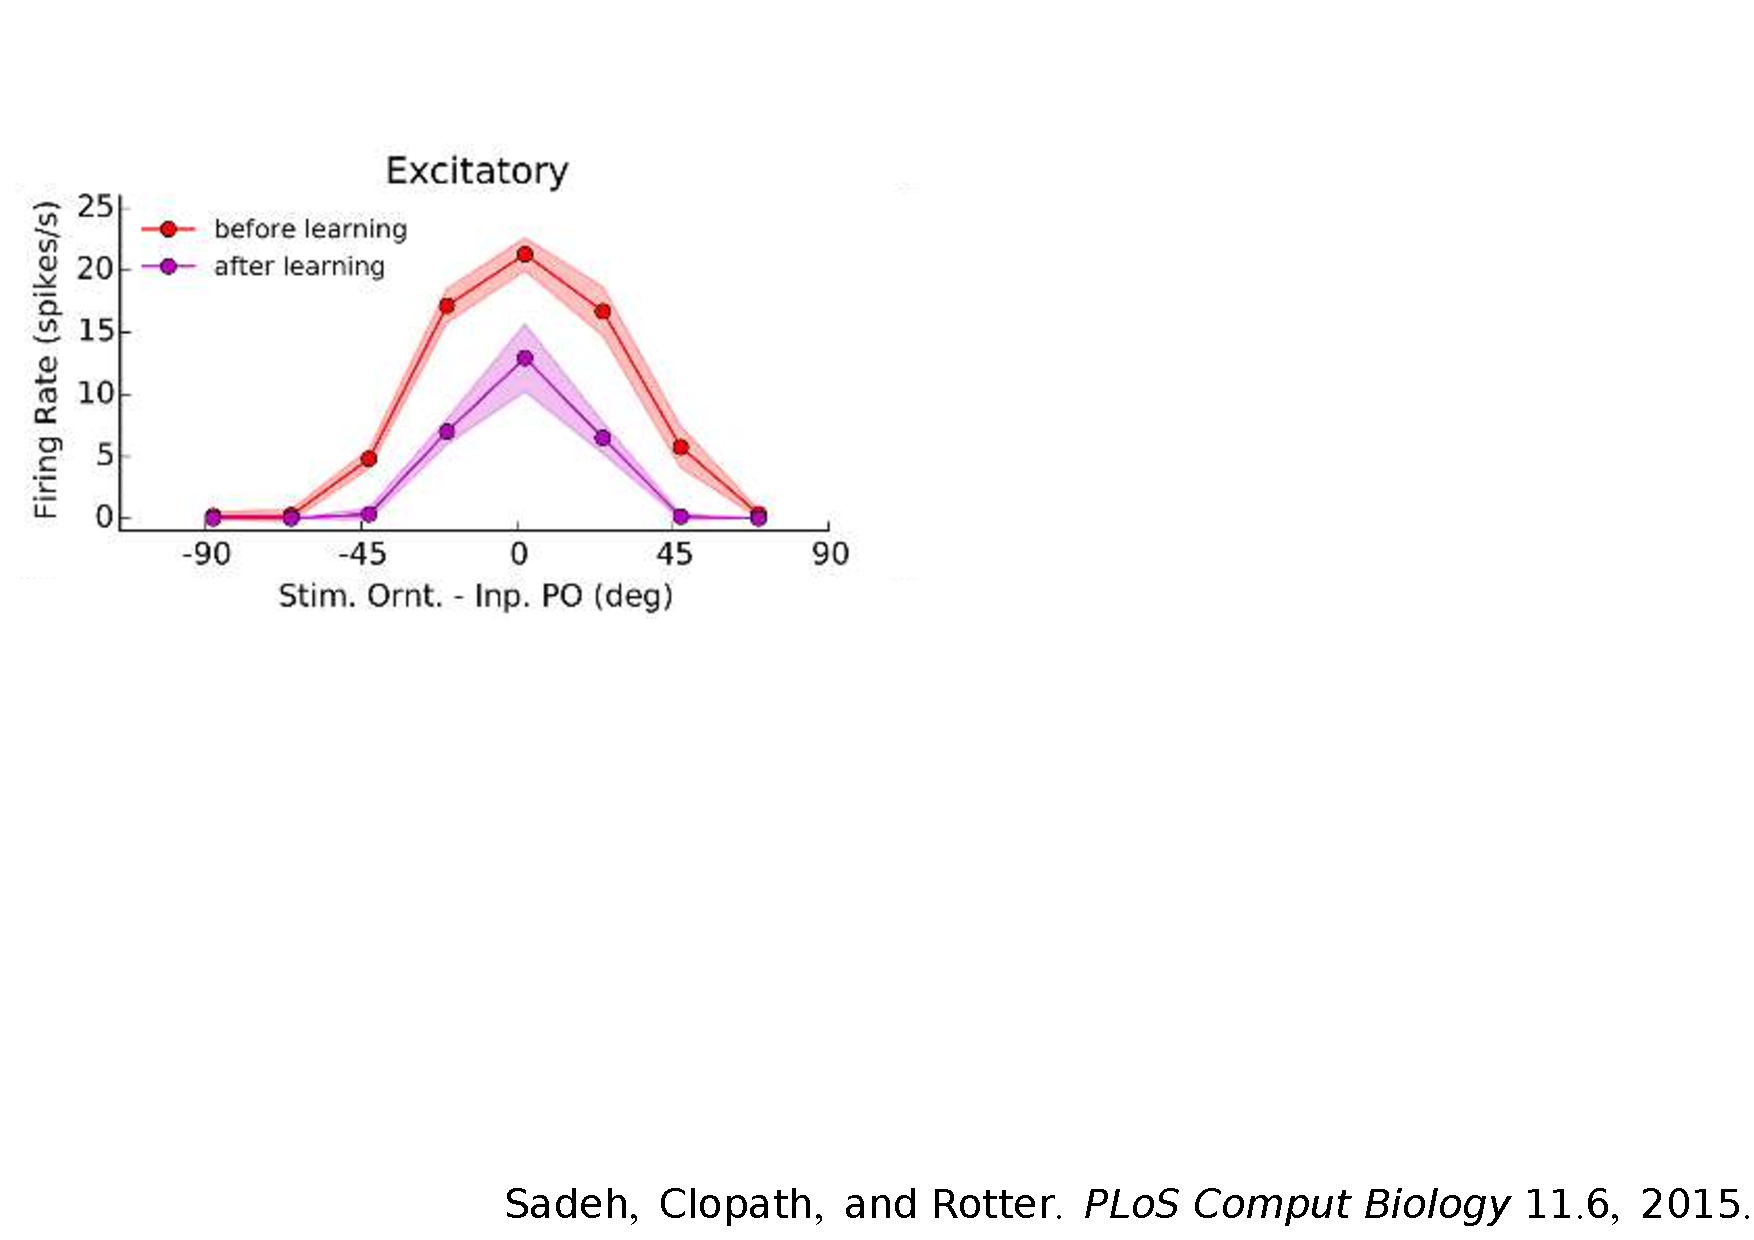
\includegraphics[height=0.9\textheight]{sadra_tuning_curves1}
    }
    \only<2>{
    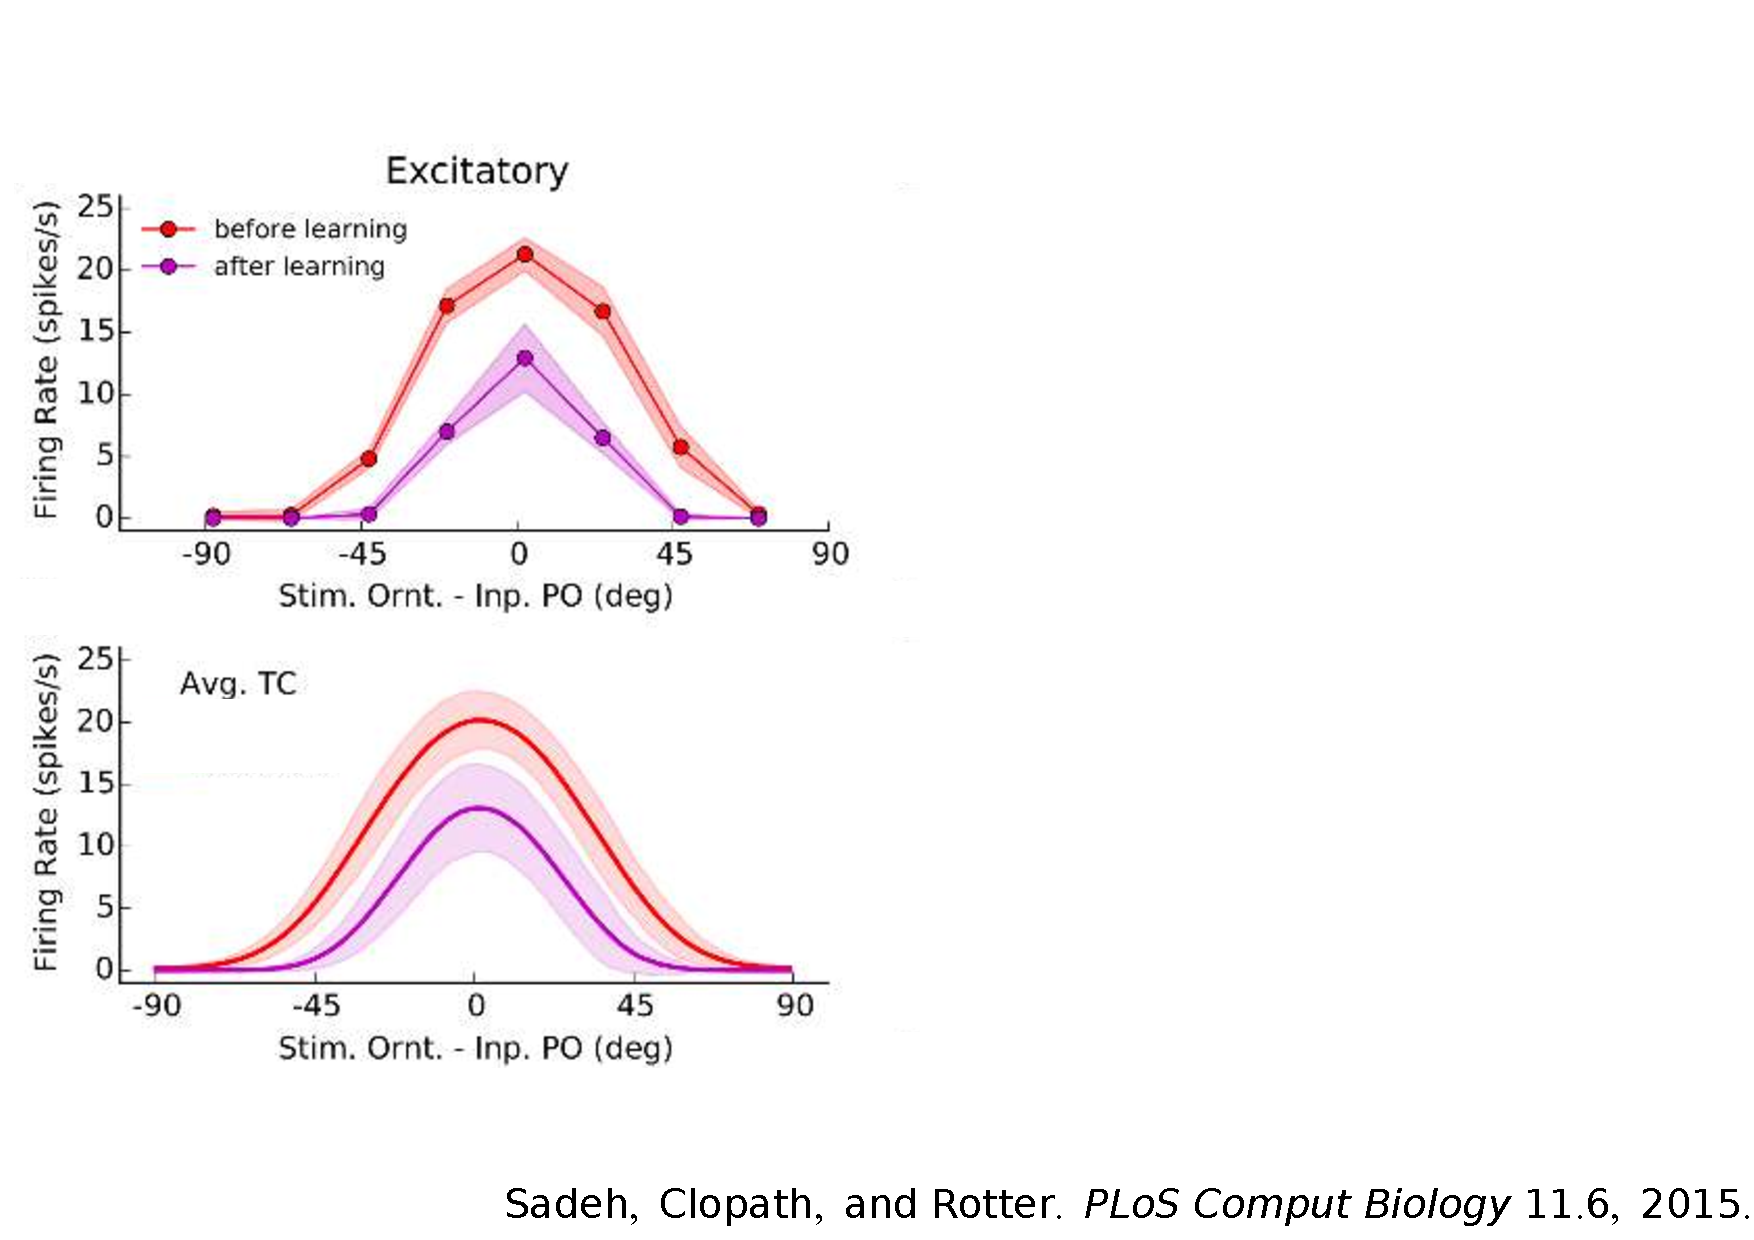
\includegraphics[height=0.9\textheight]{sadra_tuning_curves2}
    }
    \only<3>{
    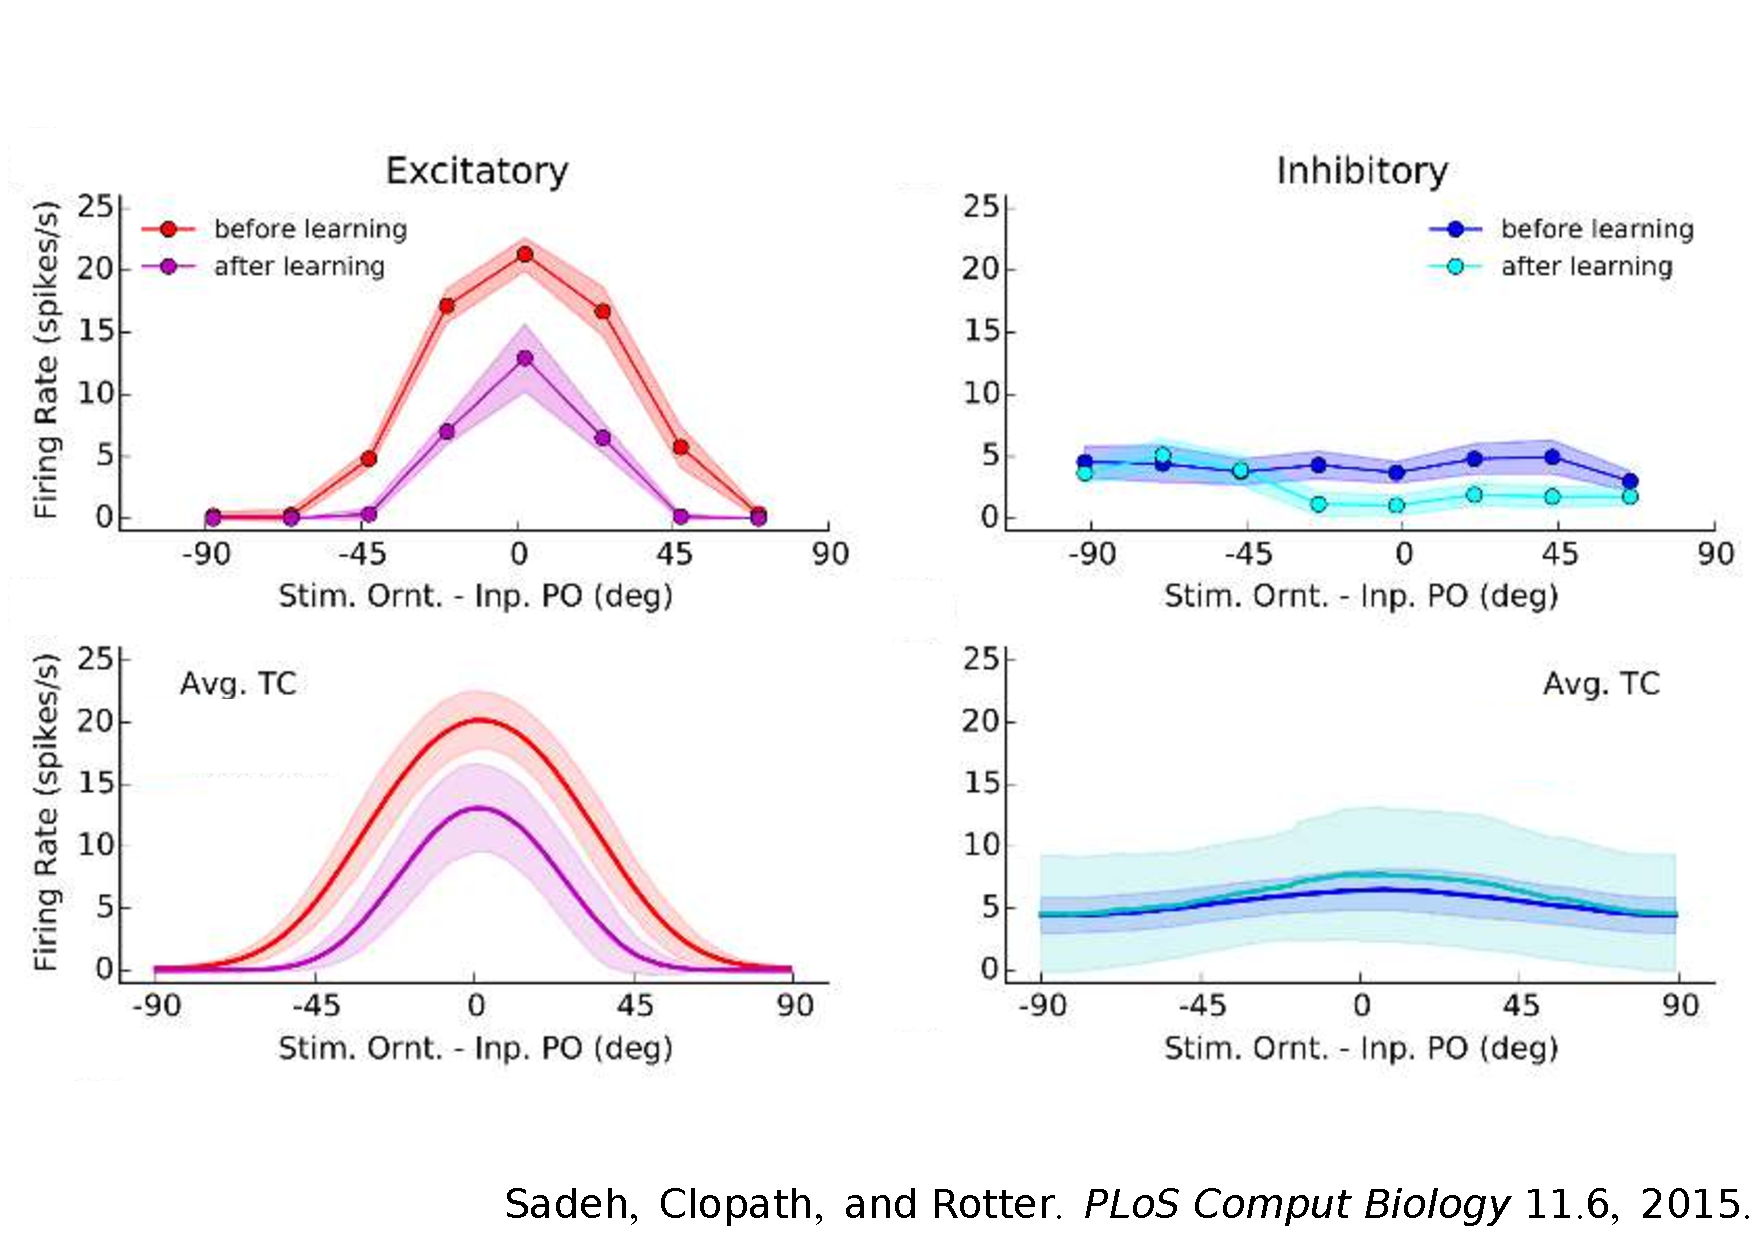
\includegraphics[height=0.9\textheight]{sadra_tuning_curves}
    }
\end{frame}

% Connectivity matrix
\begin{frame}[t]{Connectivity matrix}
    \only<1>{
    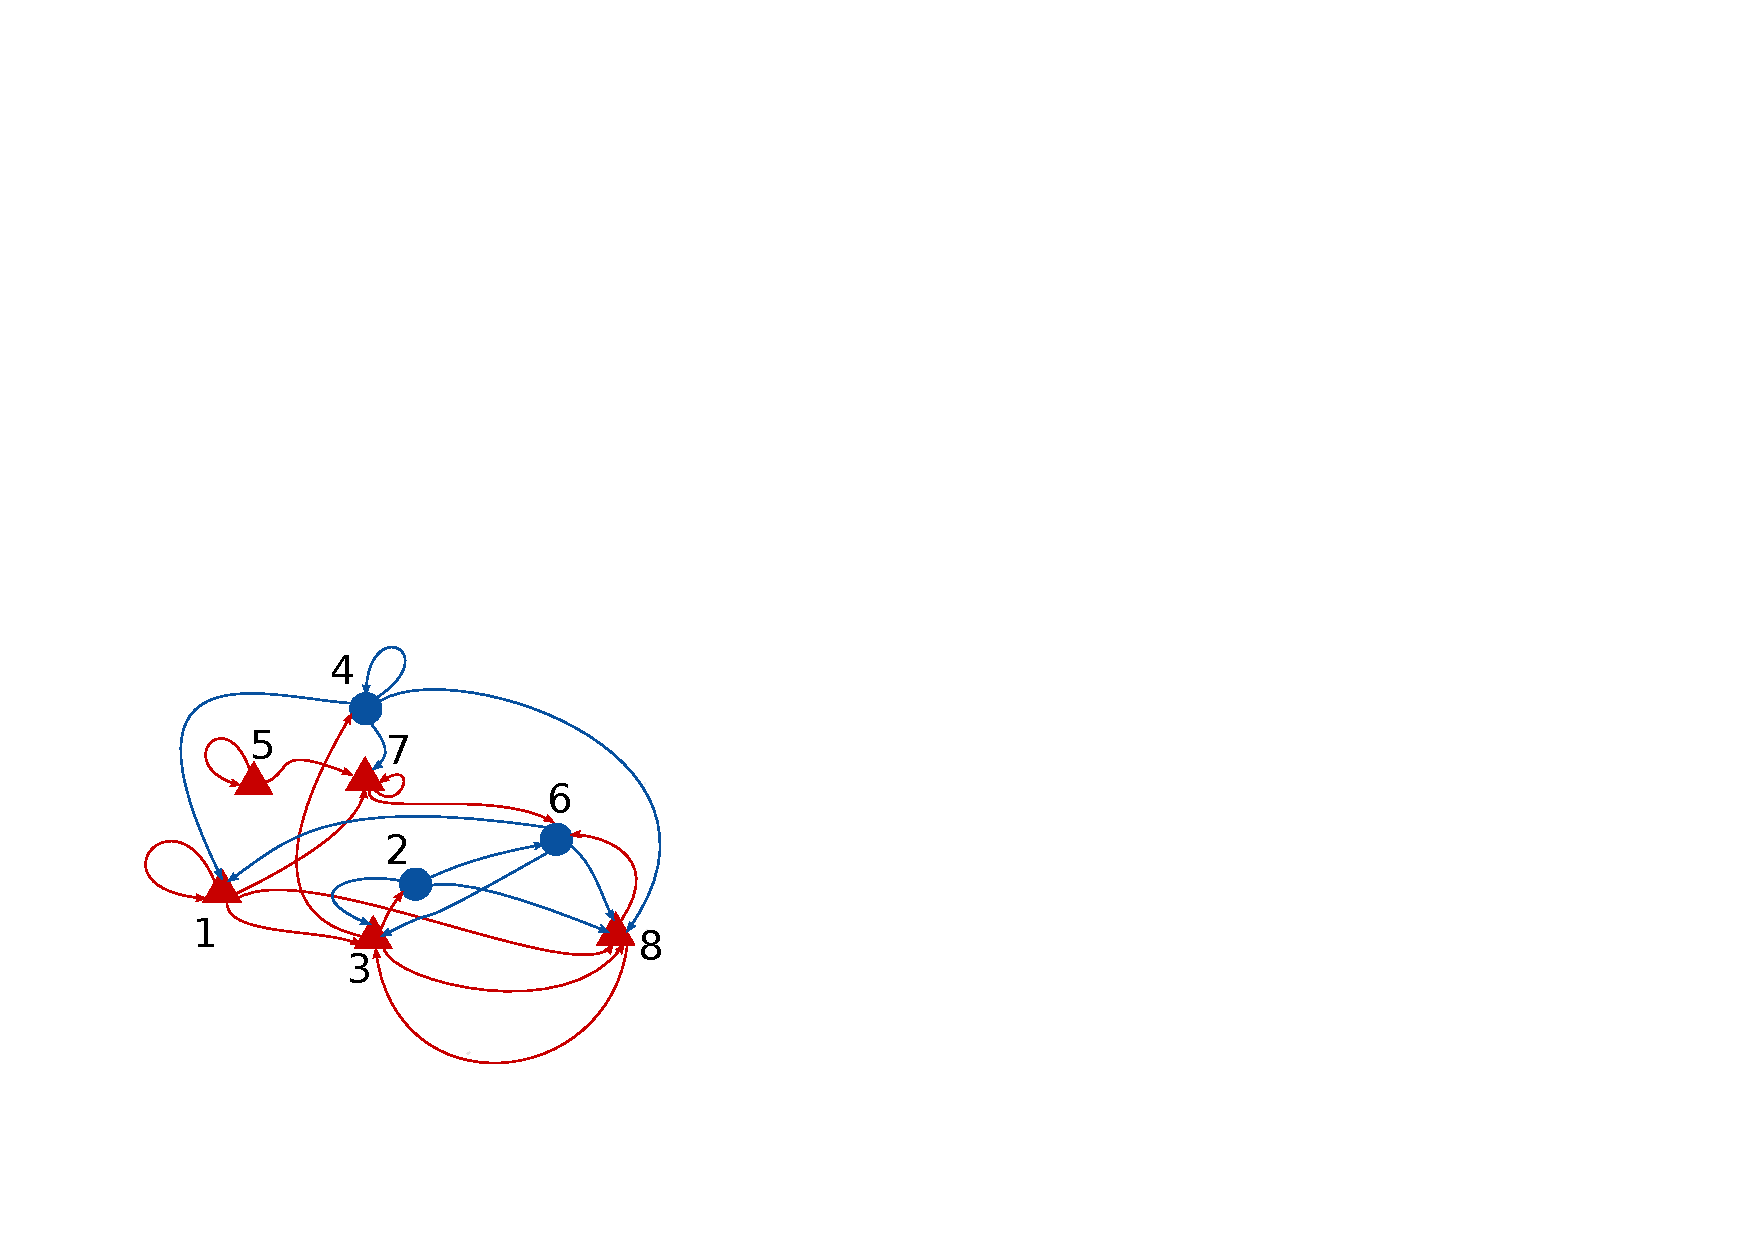
\includegraphics[height=0.9\textheight]{explain_conn_matrix1}
    }
    \only<2>{
    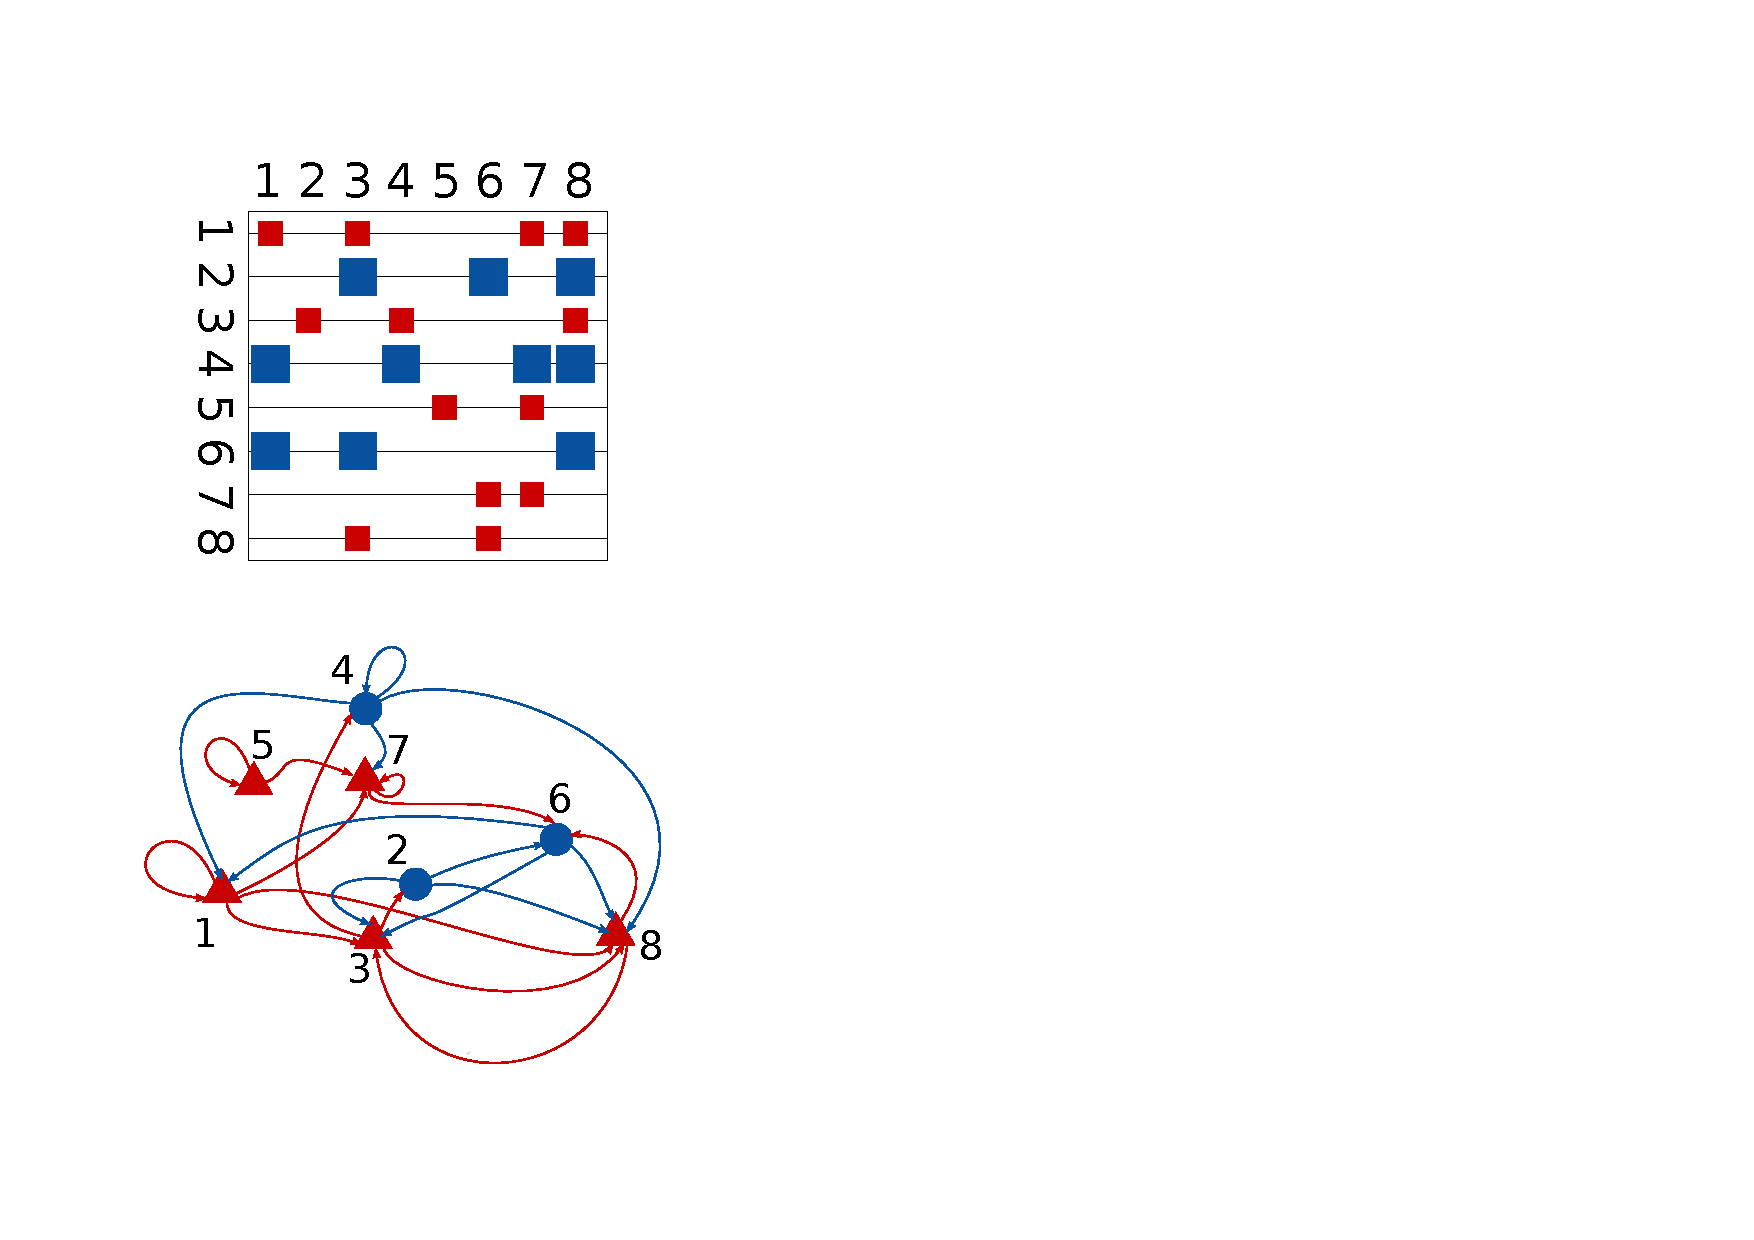
\includegraphics[height=0.9\textheight]{explain_conn_matrix2}
    }
    \only<3>{
    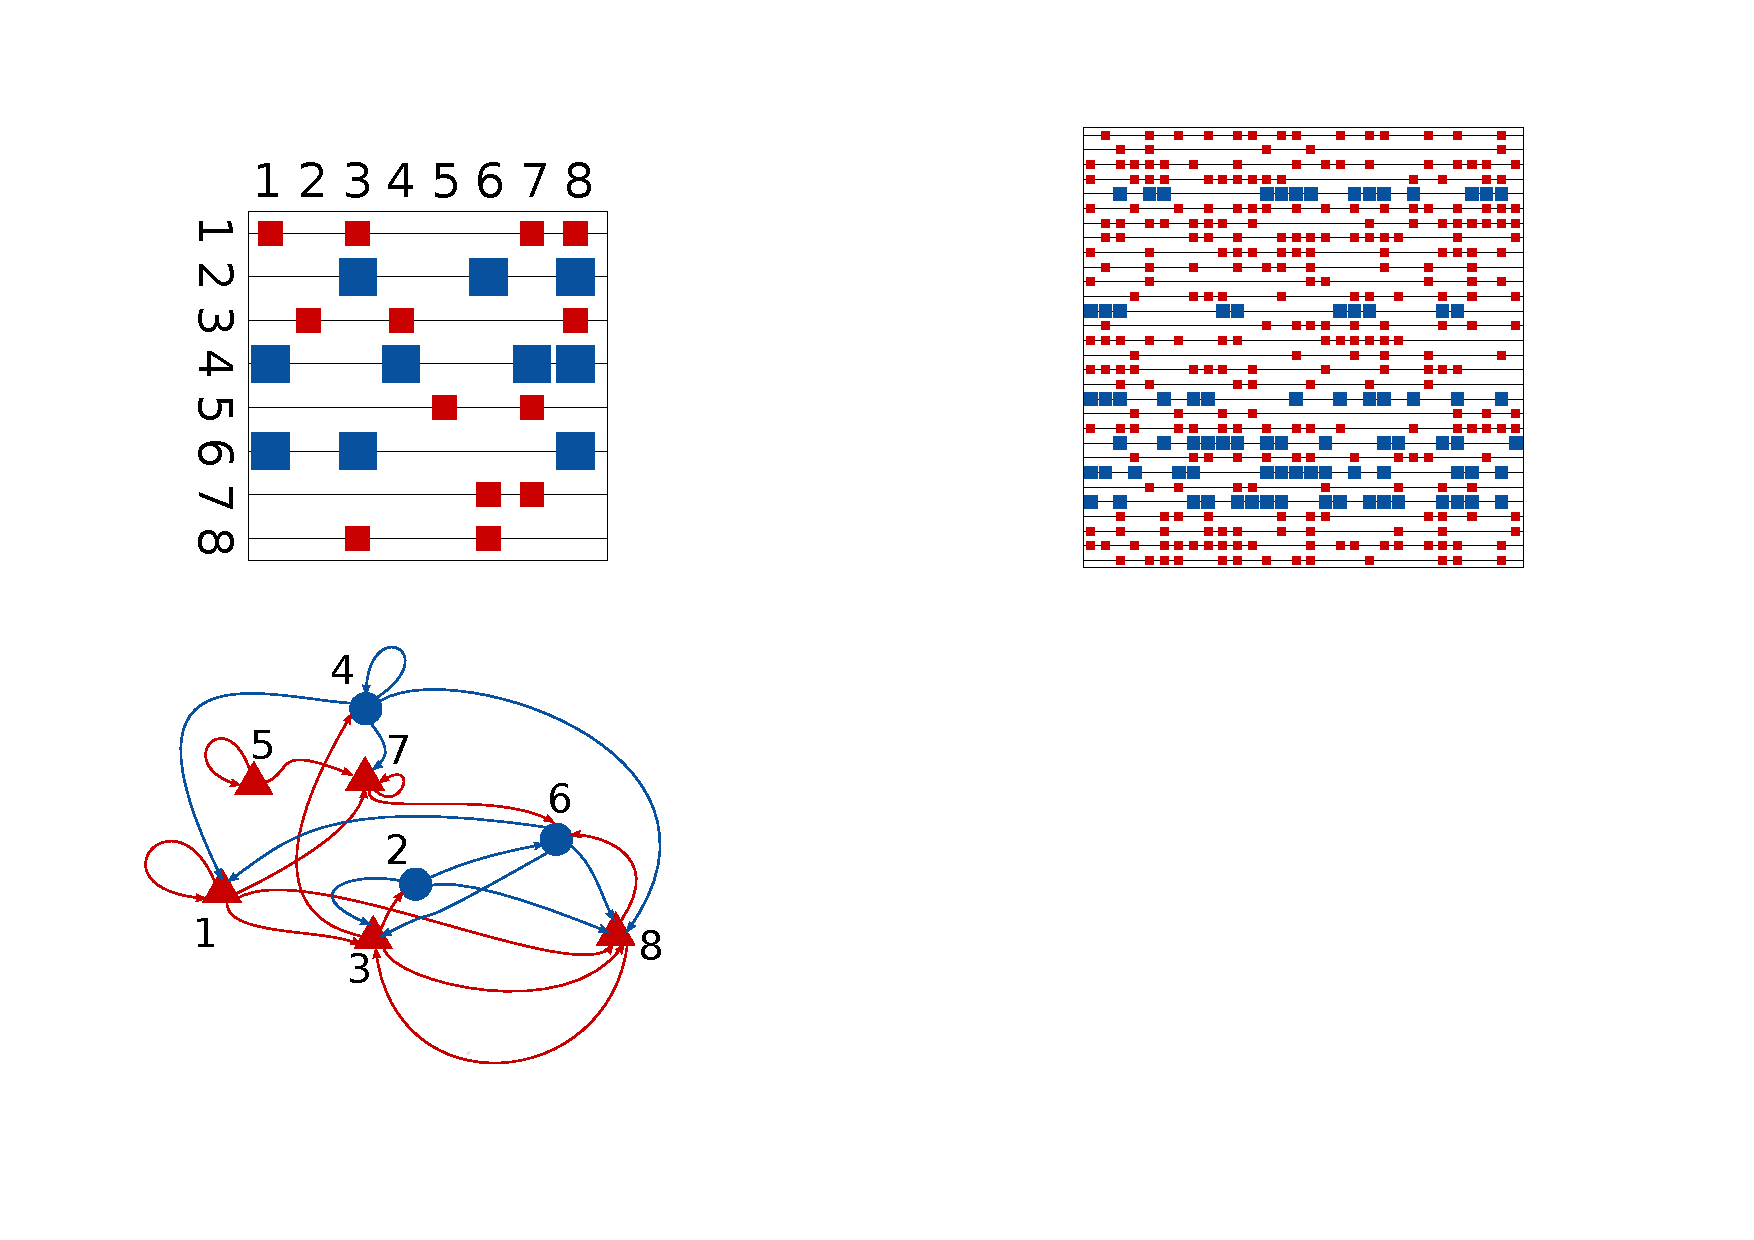
\includegraphics[height=0.9\textheight]{explain_conn_matrix3}
    }
    \only<4>{
    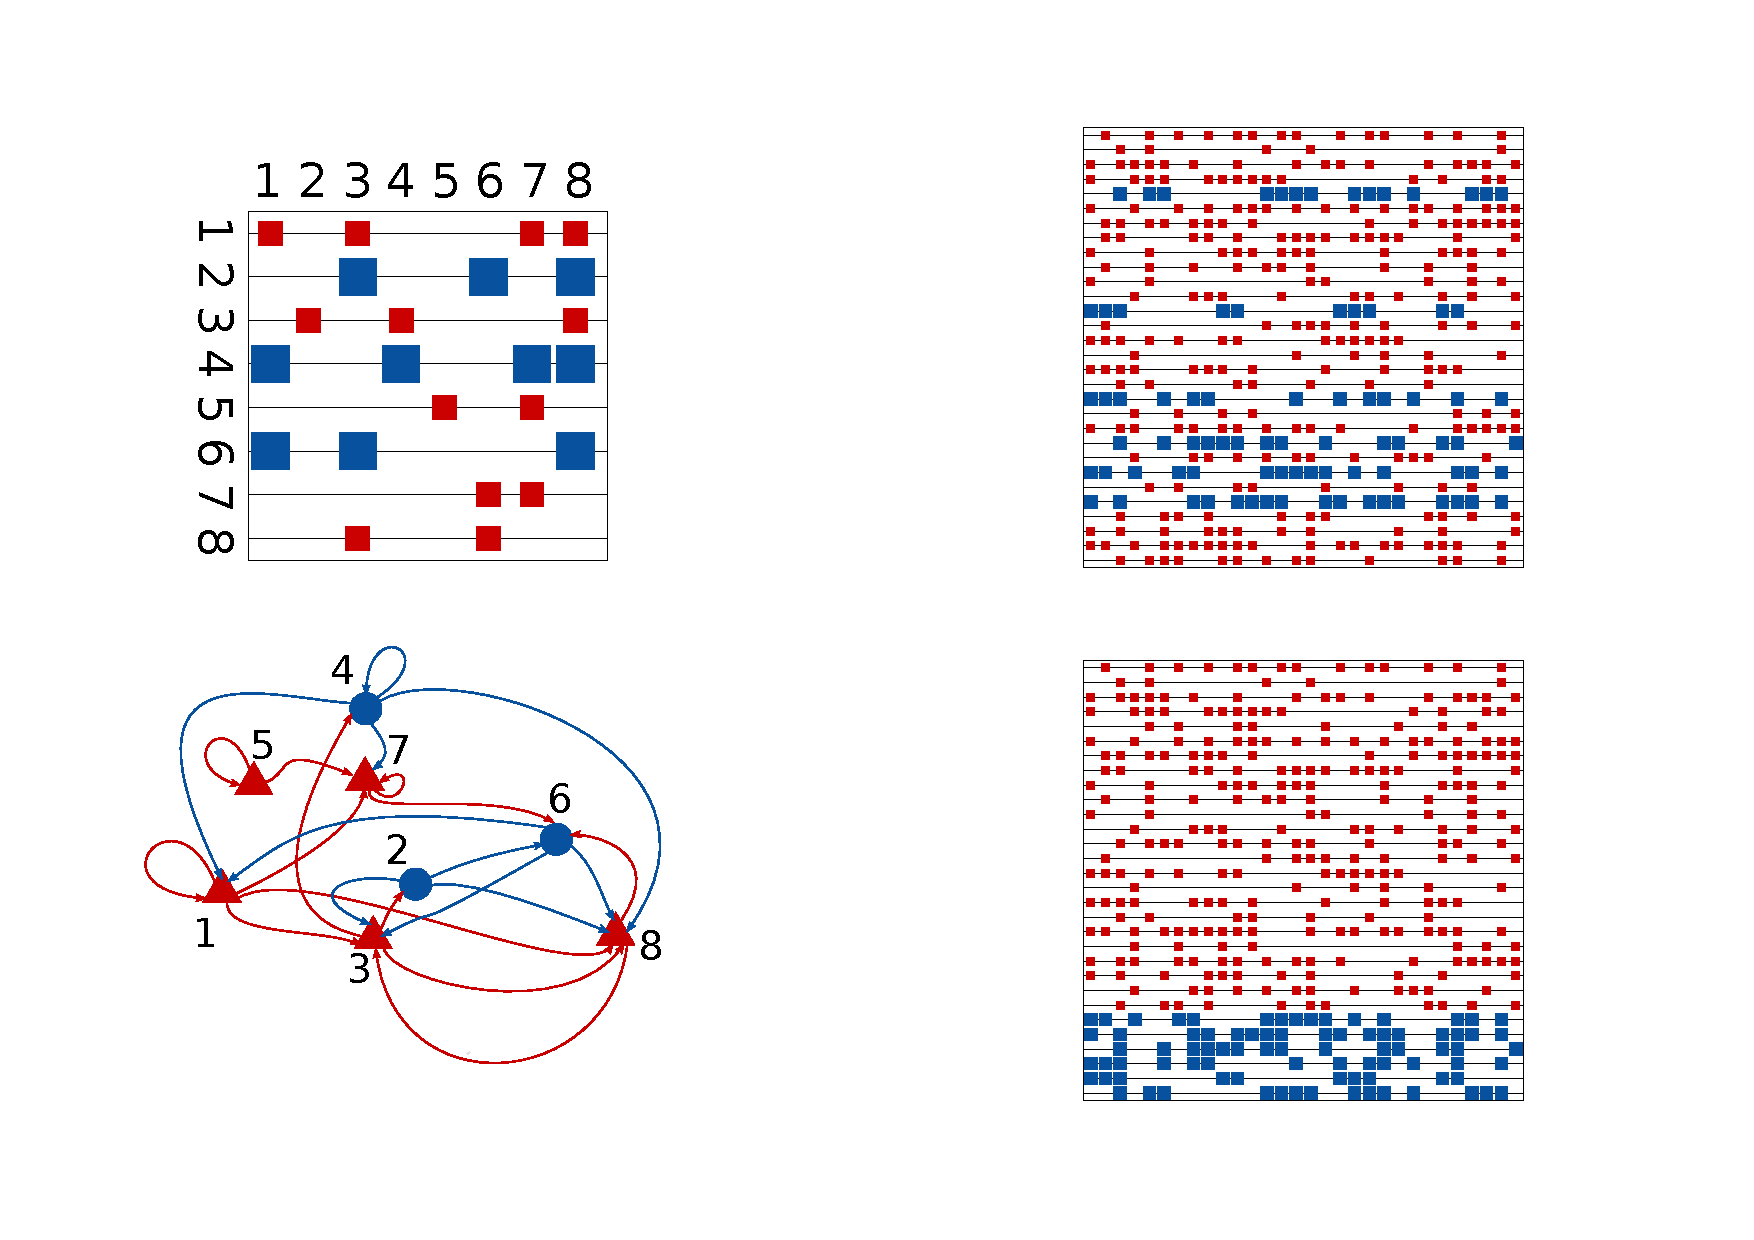
\includegraphics[height=0.9\textheight]{explain_conn_matrix}
    }
\end{frame}


\begin{frame}[t]{Changing connectivity}
    \only<1>{
    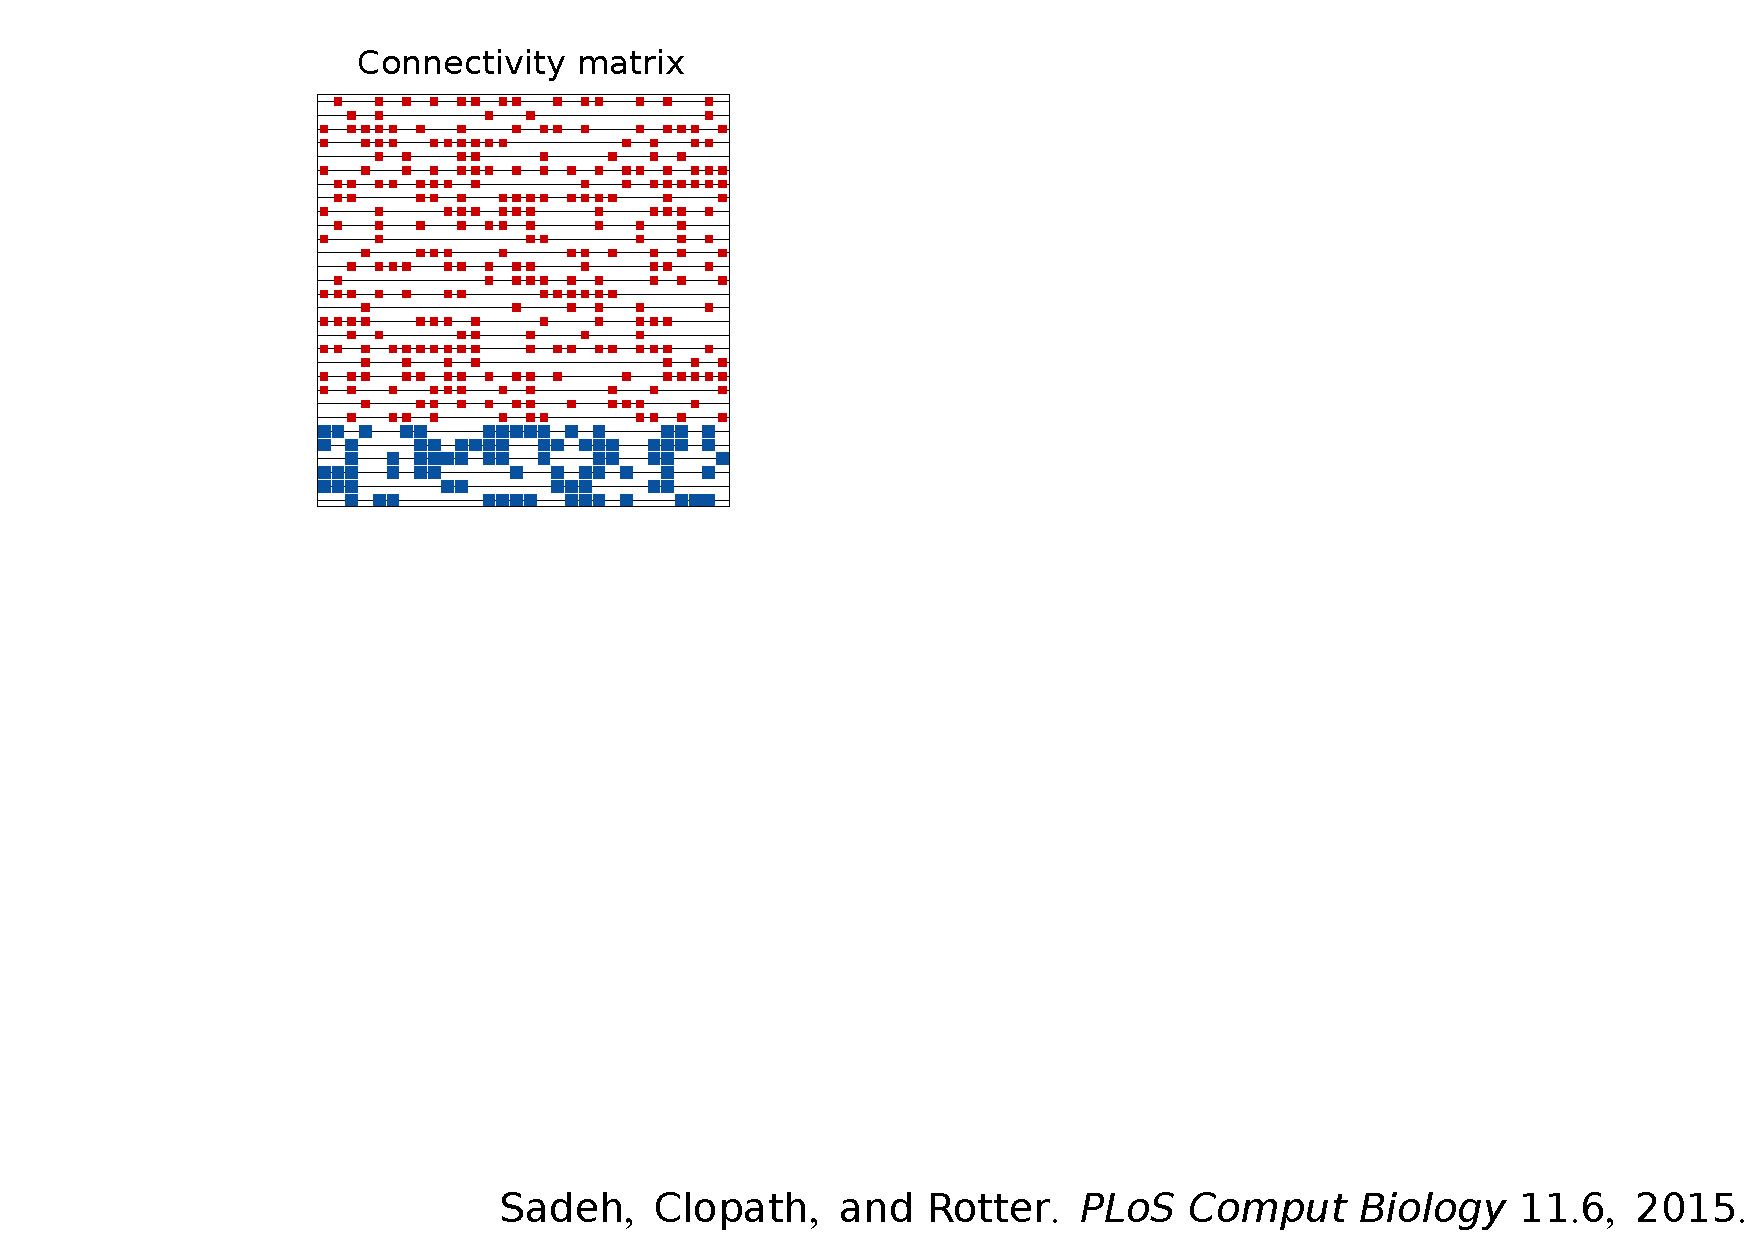
\includegraphics[height=0.9\textheight]{sadra_matrix1}
    }
    \only<2>{
    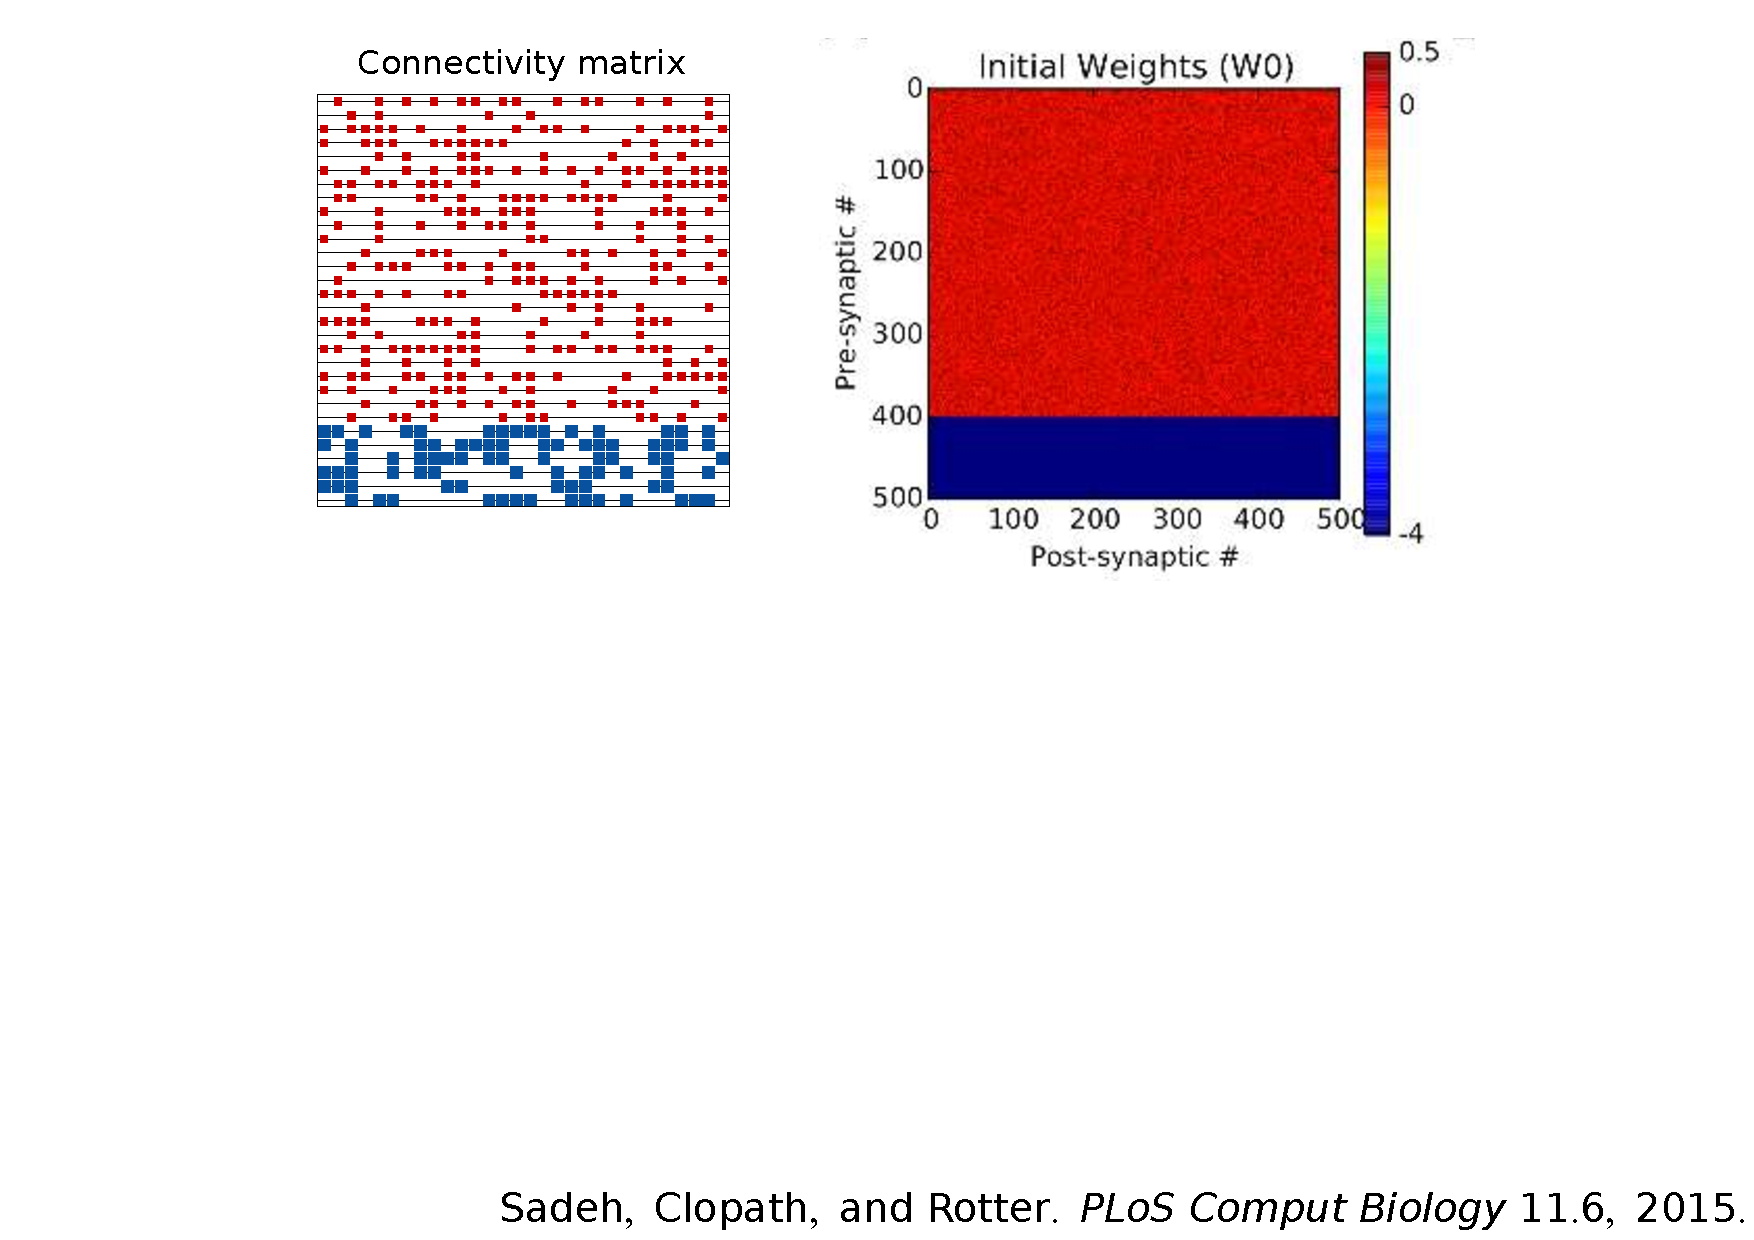
\includegraphics[height=0.9\textheight]{sadra_matrix2}
    }
    \only<3>{
    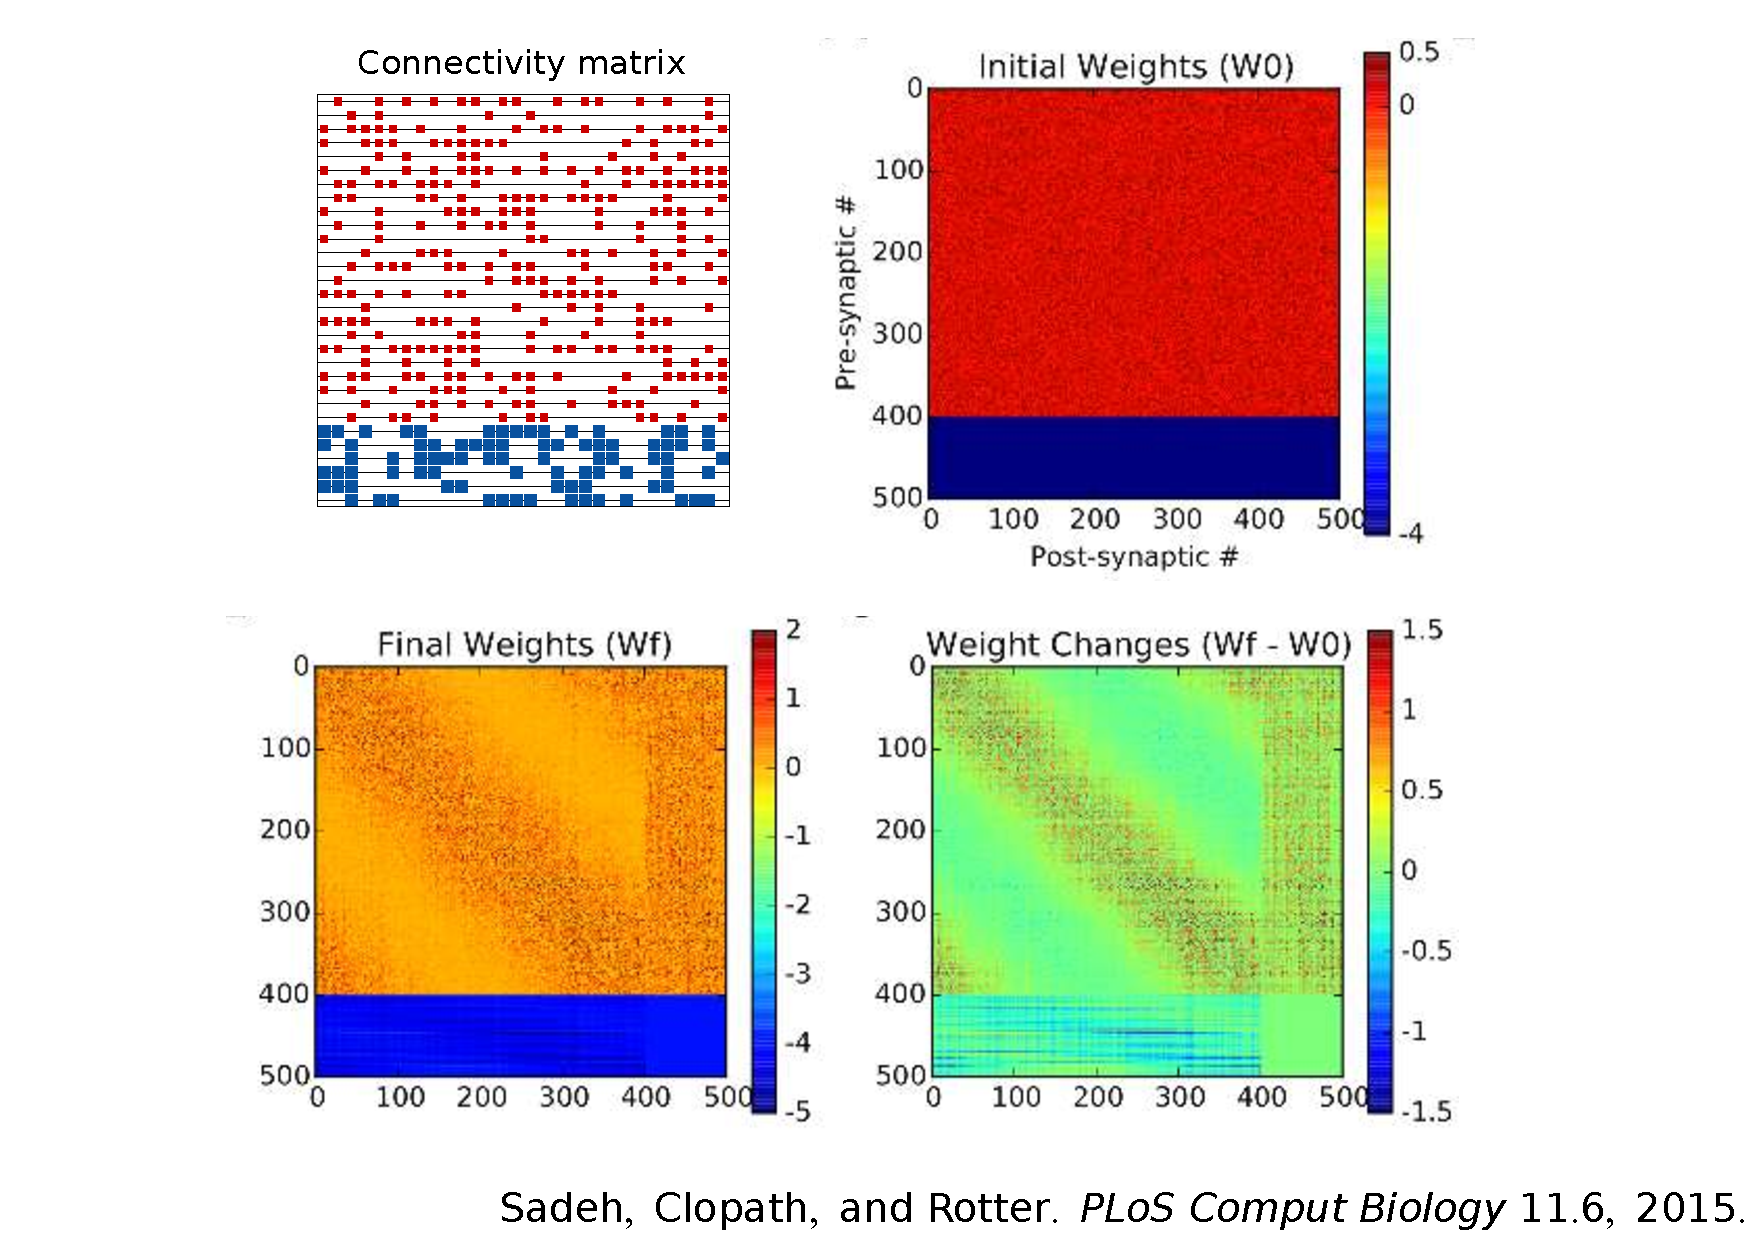
\includegraphics[height=0.9\textheight]{sadra_matrix}
    }
\end{frame}


\section{Conclusion}
\label{sec:conclusion}

% Conclusion
\begin{frame}[t]{Conclusion}
\only<1->{
    Some features exists already at birth.: Orientation selectivity. \\
}
\only<2->{
    \vspace{2cm}
    Network structure can change drastically with sensory experience:
    Feature specific microcircuits.\\ 
}
\only<3->{
    \vspace{2cm}
    Balanced random networks and synaptic plasticity may explain the
    phenomenon. \\
}
\end{frame}

% References
\begin{frame}[t]
    \frametitle<presentation>{References}    

    \scriptsize
    Basics\\
    \vspace{0.1cm}
    \tiny
    % Bear, Connors
    Bear, Mark F., Barry W. Connors, and Michael A. Paradiso, eds. 
    Neuroscience. Vol. 2. 
    \textit{Lippincott Williams \& Wilkins}, 2007.
    \vspace{0.1cm}

    % Purves
    Purves, Dale, et al.
    Neuroscience.
    \textit{Sinauer Associates, Inc.}, 2004. 
    \vspace{0.1cm}
    
    \scriptsize
    Orientation selectivity\\
    \vspace{0.1cm}
    \tiny
    % Hubel \& Wiesel
    Hubel, David H., and Torsten N. Wiesel. 
    Receptive fields of single neurones in the cat's striate cortex. 
    \textit{The Journal of physiology} 148.3, 1959.
    \vspace{0.1cm}

    % Explanation
    Hubel, David H., and Torsten N. Wiesel. 
    Receptive fields, binocular interaction and functional architecture in the cat's visual cortex.
    \textit{The Journal of physiology} 160.1, 1962.
    \vspace{0.1cm}

    %%% Experiment
    \scriptsize
    Experimental evidence:\\
    \vspace{0.1cm}
    \tiny
    % Ko et al.
    Ko, Ho, et al. 
    The emergence of functional microcircuits in visual cortex. 
    \textit{Nature} 496.7443, 2013.
    \vspace{0.1cm}

    %Calcium Imaging
    Stosiek, Christoph, et al. 
    In vivo two-photon calcium imaging of neuronal networks.
    \textit{Proceedings of the National Academy of Sciences} 100.12, 2003.
    \vspace{0.1cm}

    %%% Computer Model
    \scriptsize
    Computer model\\
    \vspace{0.1cm}
    \tiny
    %STDP Model
    Clopath, Claudia, et al. 
    Connectivity reflects coding: a model of voltage-based STDP with homeostasis.
    \textit{Nature neuroscience} 13.3, 2010.
    \vspace{0.1cm}

    % Sadra 2015
    Sadeh, Sadra, Claudia Clopath, and Stefan Rotter. 
    Emergence of Functional Specificity in Balanced Networks with Synaptic Plasticity.
    \textit{PLoS Comput Biology} 11.6, 2015.
    \vspace{0.1cm}

\end{frame}


% Last
\begin{frame}[t]{}
    
\includegraphics[height=0.9\textheight]{thank_you}
\end{frame}


%% Appendix
\section*{Appendix}
\label{sec:appendix}

% What do random networks do? : Amplification, contrast invariance
%\begin{frame}[t]{Amplification}
    %Property of random networks
%\end{frame}

%\begin{frame}[t]{Contrast Invariance}
    %2nd property
%\end{frame}

\begin{frame}[t]{Orientation selectivity}
    \only<1>{
    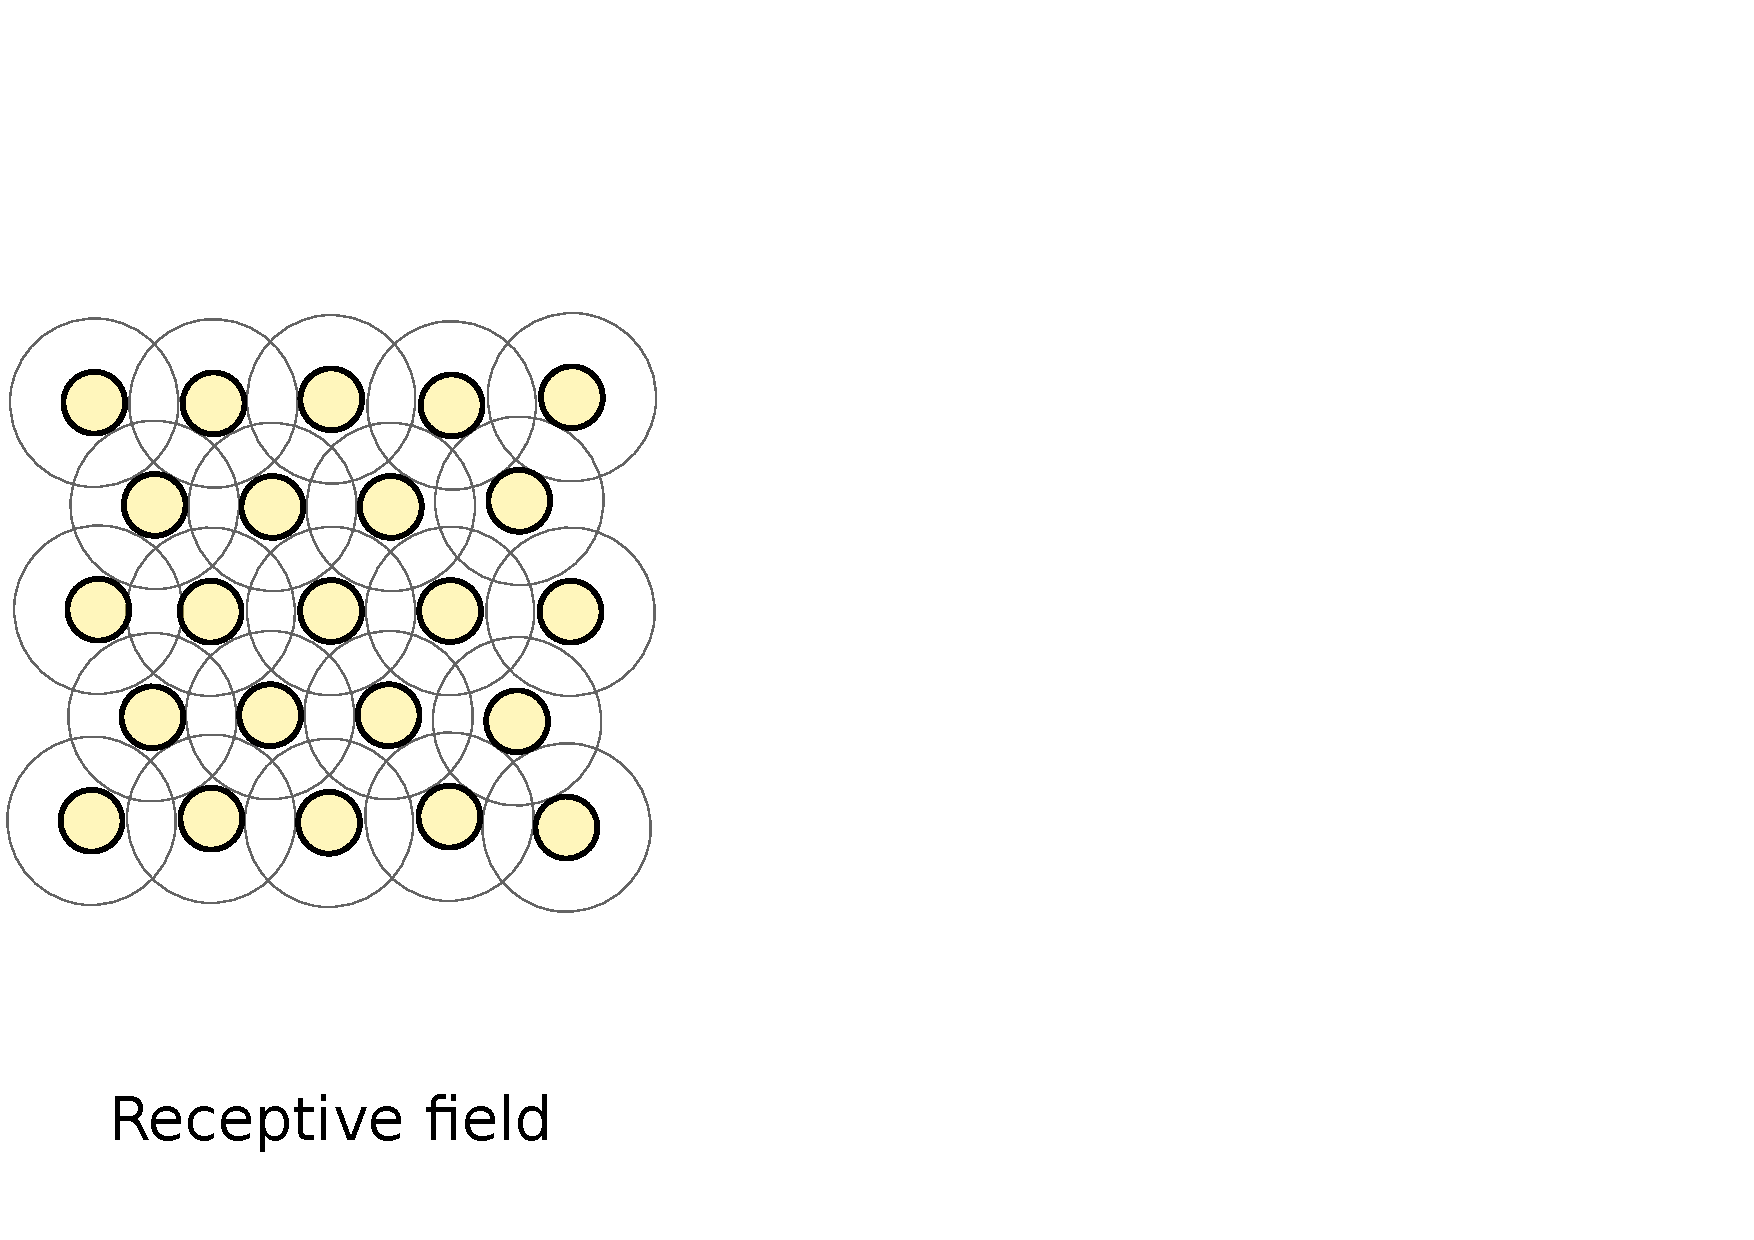
\includegraphics[height=0.9\textheight]{rf_blue1}
    }
    \only<2>{
    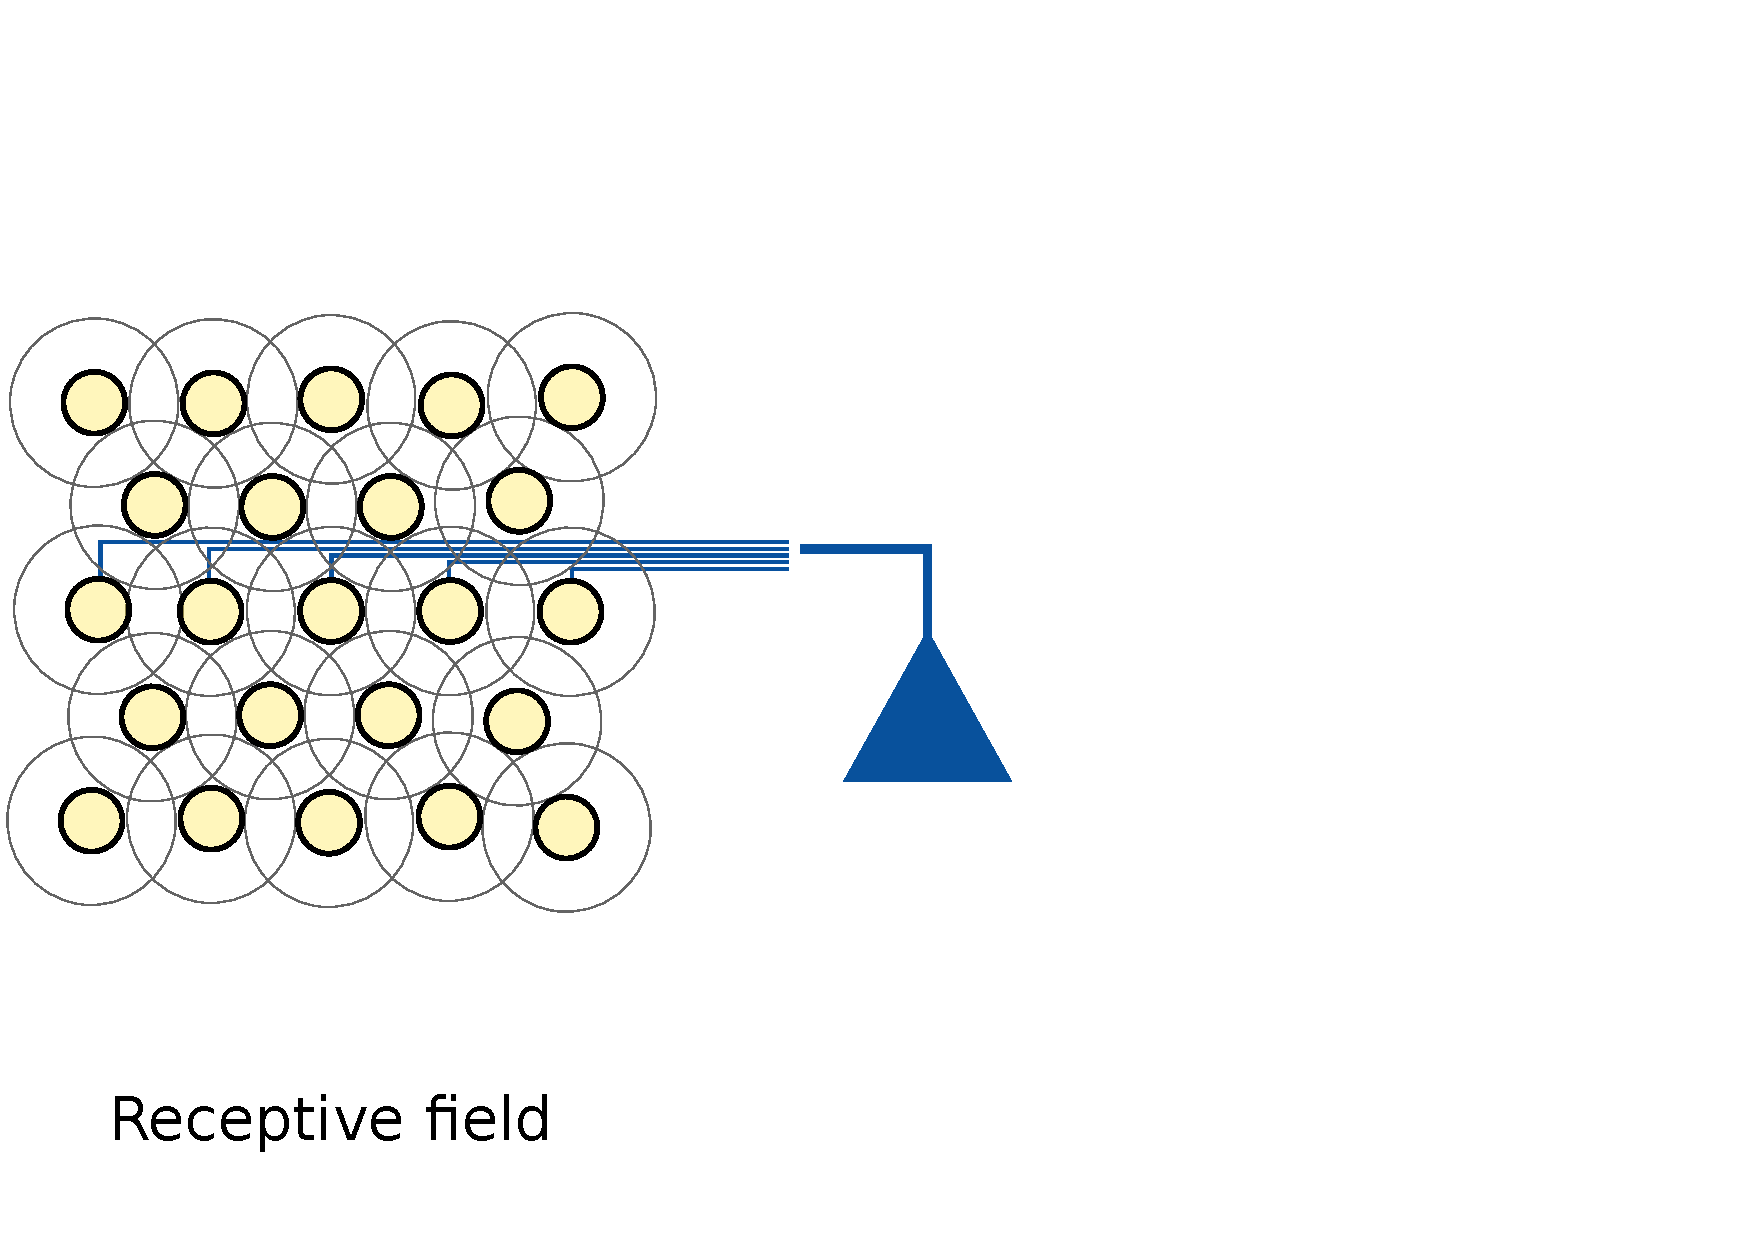
\includegraphics[height=0.9\textheight]{rf_blue2}
    }
    \only<3>{
    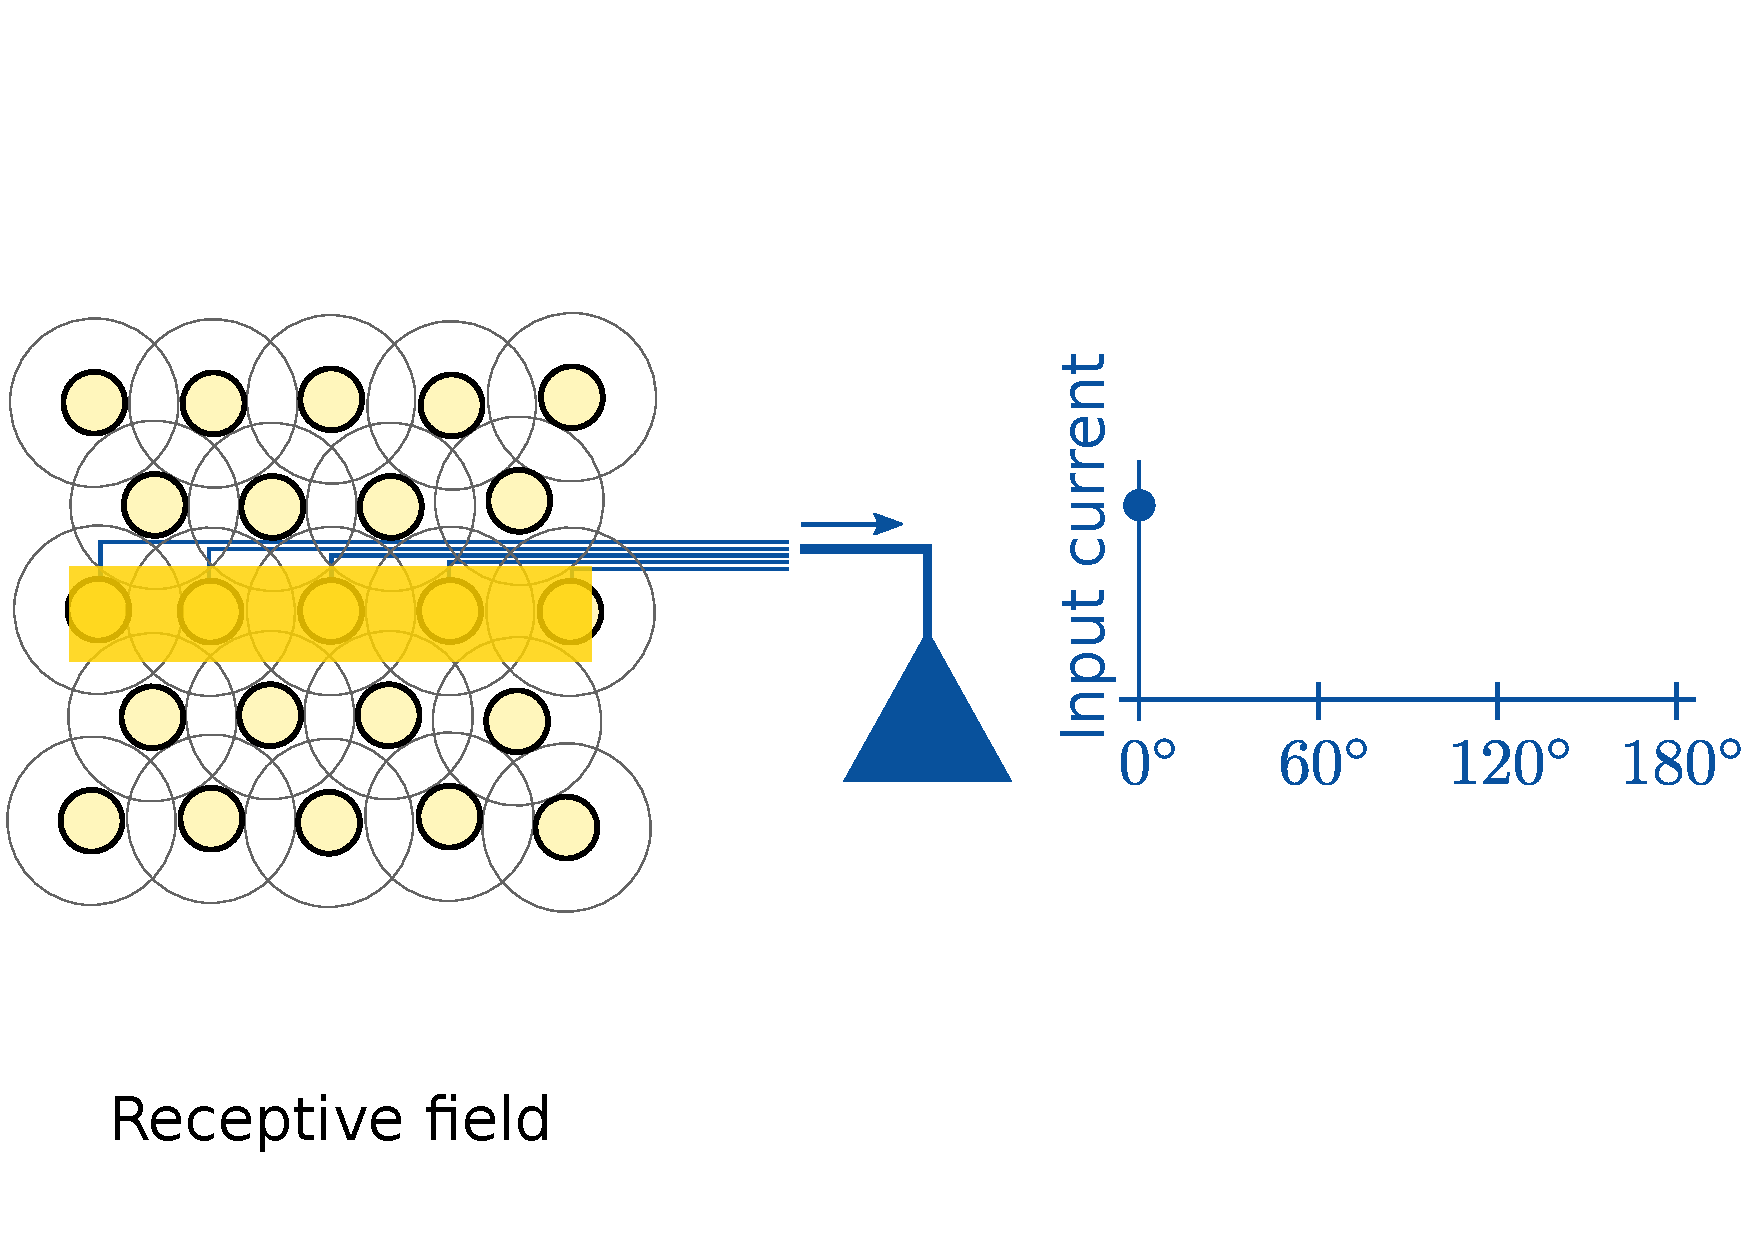
\includegraphics[height=0.9\textheight]{rf_blue3}
    }
    \only<4>{
    \includegraphics[height=0.9\textheight]{rf_blue4}
    }
    \only<5>{
    \includegraphics[height=0.9\textheight]{rf_blue5}
    }
    \only<6>{
    \includegraphics[height=0.9\textheight]{rf_blue}
    }
\end{frame}

% Principle: Tuning curves
\begin{frame}[t]{Tuning curves}
    \includegraphics[height=0.9\textheight]{receptive_fields}
\end{frame}

\end{document}
